%% FEUP THESIS STYLE for LaTeX2e
%% how to use feupteses (English version)
%% FEUP, JCL & JCF, October 2024
%%
%% Read the documentation inline and at the included `README` file
%%
%% PLEASE send improvements to jcf at fe.up.pt and to jlopes at fe.up.pt
%%

\documentclass[11pt,a4paper]{report}

%% For two-sided printing (for dead-tree output) comment previous line
%% and uncomment the next line
%\documentclass[11pt,a4paper,twoside,openright]{report}

%% Source text uses in UTF-8 encoding
\usepackage[utf8]{inputenc}
\usepackage{array}
\usepackage{booktabs}  % for \toprule etc.
\usepackage{enumitem}  % for compact itemiz

%% MESW options
\usepackage[mesw]{feupteses}              % working version
%\usepackage[mesw,juri]{feupteses}        % juri version
%\usepackage[mesw,final]{feupteses}       % final PDF version

%% Additional options for feupteses.sty:
%% - portugues: titles, etc in portuguese
%% - onpaper: links are not shown (for paper versions)
%% - backrefs: include back references from bibliography to citation place
%% - iso: format references according to ISO 690 standard

%% TIP: use folder ``figures'' to keep all your figures
%% Path to the figures directory
\graphicspath{{figures/}}

%% Change to the appropriate bibliography file
\addbibresource{bibliography.bib}

%%========================================
%% Start of document
%%========================================
\begin{document}

%%----------------------------------------
%% Information about the work
%%----------------------------------------
\title{$<$Smart-Doc: AI-Powered Medical Education through Diagnostic Interactions$>$}
\author{$<$Bruno de Sena Pereira$>$}

%% Uncomment next line for date of submission
%\thesisdate{July 31, 2008}

%% Comment next line copyright text if not used
\copyrightnotice{Bruno de Sena Pereira, 2025}

\supervisor{Supervisor}{Prof.\ $<$Nuno Freixa$>$}

%% Uncomment next line if necessary
%\supervisor{Second Supervisor}{Prof.\ $<$Name of the Supervisor$>$}

%% Uncomment committee stuff in the final version if used
%\committeetext{Approved in oral examination by the committee:}
%\committeemember{President}{Prof.\ $<$Name of the Professor$>$}
%\committeemember{Referee}{Prof.\ $<$Name of the Professor$>$}
%\committeemember{Referee}{Prof.\ $<$Name of the Professor$>$}

%% uncomment next line to draw line for handwritten signature (if necessary)
%\signature

%% Specify cover logo (in folder ``figures'')
\logo{uporto-feup.pdf}

%% Uncomment next line for additional text below the author's name (front page)
%\additionalfronttext{<Additional text>}

%%----------------------------------------
%% Preliminary materials
%%----------------------------------------

% remove unnecessary \include{} commands
\begin{Prolog}
  %% abstract.tex: abstract in PT and EN  (FEUP regulations)
%% -------------------------------------------------------
\chapter*{Resumo}
%
\newpage

\chapter*{Abstract}
%
\newpage % the abstract
  %% un-sdg.tex: UN Sustainable Development Goals (FEUP regulations)
%% -------------------------------------------------------

\chapter*{UN Sustainable Development Goals} \label{chap:UnitedNations}

The United Nations Sustainable Development Goals (SDGs) provide a global framework to achieve a better and more sustainable future for all. 
It includes 17 goals to address the world's most pressing challenges, including poverty, inequality, climate change, environmental degradation, peace, and justice. 

Quisque ullamcorper placerat ipsum. Cras nibh. Morbi vel justo vitae lacus tincidunt ultrices.
Lorem ipsum dolor sit amet, consectetuer adipiscing elit. 
In hac habitasse platea dictumst. Integer tempus convallis augue. Etiam facilisis. 

The specific Sustainable Development Goals mentioned have the following names:

\begin{description}
\item [SDG 7]
Ensure access to affordable, reliable, sustainable and modern energy for all
\item [SDG 8]
Promote sustained, inclusive and sustainable economic growth, full and productive employment and decent work for all
\end{description}

\begin{center}
\begin{tabular}{|l|l|p{58mm}|p{52mm}|}
\hline
\textbf{SGD} & \textbf{Target} & \textbf{Contribution} & \textbf{Performance Indicators and Metrics} \\ 
\hline
\hline
    \multirow{3}{*}{7} & 7.1 & Enhancing the efficiency of SCADA systems can help increase the reliability of solar energy production, facilitating universal access to clean energy. & Percentage of solar plants with improved \ldots \\
    \cline{2-4}
    & 7.2 & Improving the management of solar plants helps enhance the efficiency and reliability of renewable energy \ldots & Increase in renewable energy share \ldots \\
\hline
    \multirow{2}{*}{8} & 8.1 & Enhancing renewable energy infrastructure promotes resilience against climate-related hazards and supports sustainable energy sources. & Increase in resilience metrics \ldots \\
\hline
\end{tabular}
\end{center}   % United Nations Sustainable Development Goals (SGD)
  \chapter*{Acknowledgements}
%\addcontentsline{toc}{chapter}{Acknowledgements}

\newpage

\vspace{10mm}
\flushleft{$<$O Nome do Autor$>$}
  % the acknowledgments
  %% This section is optional and can be removed
\cleardoublepage
\thispagestyle{plain}

\vspace*{8cm}

\begin{flushright}
   \textsl{``Our greatest glory is not in never falling, but in rising every time we fall''} \\
\vspace*{1.5cm}
    Confucius
\end{flushright}
    % initial quotation if desired
  \cleardoublepage
  %% Uncomment next line for PT
  %\renewcommand{\contentsname}{Índice}
  \pdfbookmark[0]{Table of Contents}{contents}
  \tableofcontents
  \cleardoublepage
  \pdfbookmark[0]{List of Figures}{figures}
  \listoffigures
  \cleardoublepage
  \pdfbookmark[0]{List of Tables}{tables}
  \listoftables
  %% Abbreviations are in the `abbrevs.tex' file
  %% Omit if there aren't any
  \chapter*{List of Acronyms}
\chaptermark{LIST OF ACRONYMS}

\begin{flushleft}
\begin{tabular}{l p{0.75\linewidth}}
AI        & Artificial Intelligence \\
API       & Application Programming Interface \\
AR        & Analytical Reasoning (System~2) \\
ASR       & Automatic Speech Recognition \\
BNP       & Brain Natriuretic Peptide \\
CDM       & Clinical Decision-Making \\
CFS       & Cognitive Forcing Strategies \\
CoT       & Chain-of-Thought \\
COVID-19  & Coronavirus Disease 2019 \\
CSS       & Cascading Style Sheets \\
CT        & Computed Tomography \\
CUQ       & Chatbot Usability Questionnaire \\
CXR       & Chest X-Ray \\
GPT       & Generative Pre-trained Transformer \\
Hb        & Hemoglobin \\
HF        & Heart Failure \\
HPI       & History of Present Illness \\
ICC       & Intraclass Correlation Coefficient \\
ILD       & Interstitial Lung Disease \\
IQR       & Interquartile Range \\
ITS       & Intelligent Tutoring System \\
JSON      & JavaScript Object Notation \\
LLM       & Large Language Model \\
\end{tabular}
\end{flushleft}

\newpage


\begin{flushleft}
\begin{tabular}{l p{0.75\linewidth}}
NAR       & Non-Analytical Reasoning \\
NASA-TLX  & National Aeronautics and Space Administration Task Load Index \\
NLP       & Natural Language Processing \\
NLU       & Natural Language Understanding \\
PE        & Pulmonary Embolism \\
PMH       & Past Medical History \\
QUIS      & Questionnaire for User Interaction Satisfaction \\
RA        & Rheumatoid Arthritis \\
RAG       & Retrieval-Augmented Generation \\
RCT       & Randomized Controlled Trial \\
RLHF      & Reinforcement Learning from Human Feedback \\
RNN       & Recurrent Neural Network \\
RQ        & Research Question \\
SQL       & Structured Query Language \\
SUS       & System Usability Scale \\
TB        & Tuberculosis \\
TNF       & Tumor Necrosis Factor \\
UI        & User Interface \\
UX        & User Experience \\
VP        & Virtual Patient \\
VR        & Virtual Reality \\
VSP       & Virtual Standardized Patient \\
WBC       & White Blood Cell \\
\end{tabular}
\end{flushleft}  % the list of abbreviations used
\end{Prolog}

%%----------------------------------------
%% Body
%%----------------------------------------
\StartBody

%% TIP: use a separate file for each chapter
\chapter{Introduction} 
\label{chap:chap1}

Diagnostic error is one of the most persistent threats to patient safety, with
cognitive biases recognised as a major contributor to avoidable harm in clinical
practice~\parencite{graber_diagnostic_2005}. These biases—systematic deviations
from rational judgement—can derail even experienced clinicians, leading to
premature closure of reasoning, selective information use, or overconfidence in
a favoured hypothesis. As \textcite{croskerry_importance_2003} emphasises,
traditional training methods are often insufficient to help students recognise
and mitigate these cognitive pitfalls under the pressures of real-world practice.

At the same time, the transition from medical student to competent clinician
demands the development of robust clinical reasoning skills that combine
knowledge, pattern recognition, and reflective awareness~\parencite{audetat_diagnosis_2017}.
Conventional educational approaches emphasise outcomes, but often fail to make
the \emph{process} of reasoning visible, let alone directly train learners to
detect and counteract bias in their own thinking. Addressing this unmet need
requires pedagogical approaches that can elicit reasoning patterns, expose bias,
and scaffold reflection in a safe and scalable way.

This dissertation introduces \textbf{SmartDoc}, an AI-powered virtual patient
platform designed to meet this challenge. By harnessing large language models
(LLMs), SmartDoc provides naturalistic clinical interview simulations that not
only mirror the complexity of patient interaction, but also embed mechanisms to
detect cognitive biases in real time. Beyond replication of encounters, the
system delivers structured metacognitive feedback, prompting learners to reflect
on their reasoning. In this way, SmartDoc moves beyond teaching \emph{what} to
diagnose, toward teaching \emph{how} to think—directly addressing the root
causes of diagnostic error in a controlled, scalable environment
~\parencite{mamede_structure_2004,berge_cognitive_2013}.

\section{Motivation} 
\label{sec:se1}

The motivation for this research arises from two converging forces. First, an
educational gap: reasoning errors, rather than knowledge deficits, account for a
substantial proportion of diagnostic mistakes, yet medical training rarely
provides explicit support for bias awareness~\parencite{berge_cognitive_2013}.
Second, a technological opportunity: the rapid maturation of LLMs, together with
pedagogical frameworks from Intelligent Tutoring Systems (ITS), offers a new
toolkit for building simulations that combine realism with adaptive, reflective
support. SmartDoc is situated at the intersection of these forces: a system that
leverages AI to elicit naturalistic reasoning behaviour, surface bias-prone
moments, and scaffold reflective practice.

\section{Research Questions} 
\label{sec:rq}

The central research problem guiding this dissertation is: 

\begin{quote}
\textit{How can AI-powered virtual patients be designed to help medical students
recognise and mitigate cognitive biases in their diagnostic reasoning?}
\end{quote}

From this problem, three research questions (RQs) emerge:

\begin{itemize}
    \item \textbf{RQ1:} To what extent can an LLM-powered simulation realistically
    elicit and detect cognitive biases in diagnostic interviews?
    \item \textbf{RQ2:} How effective are metacognitive prompts—delivered in real
    time or post-hoc—in fostering reflection and reducing diagnostic bias?
    \item \textbf{RQ3:} What technical and pedagogical design principles enable
    the scalable deployment of bias-aware virtual patient simulations?
\end{itemize}

\section{Objectives} 
\label{sec:ae2}

In alignment with these questions, the dissertation pursues the following
objectives:

\begin{itemize}
\item \textbf{Simulation} --- To design and implement an AI-powered virtual
patient platform capable of conducting realistic, unscripted clinical interviews
based on authentic case scenarios engineered to elicit bias.
\item \textbf{Bias Detection} --- To embed mechanisms for identifying behavioural
markers of anchoring, confirmation bias, and premature closure in learner
interactions, using a combination of rule-based and LLM-supported approaches.
\item \textbf{Metacognitive Tutoring} --- To provide context-aware prompts that
stimulate reflection and encourage reconsideration of reasoning pathways when
bias-prone behaviour is detected.
\item \textbf{Evaluation Framework} --- To develop analytics that assess
diagnostic accuracy, information-gathering behaviours, and manifestations of
cognitive bias, enabling both formative and summative feedback.
\item \textbf{Effectiveness Study} --- To conduct a pilot evaluation of the
system with clinical interns, assessing usability, educational effectiveness,
and potential impact on bias awareness.
\end{itemize}

\section{Dissertation Structure} 
\label{sec:structure}

The remainder of this dissertation is organised as follows:

\begin{itemize}
    \item \textbf{Chapter 2} presents the theoretical background, outlining
    clinical reasoning, dual-process theory, and the taxonomy of cognitive
    biases, and introducing debiasing strategies and simulation principles that
    underpin SmartDoc’s design.
    \item \textbf{Chapter 3} reviews empirical evidence on AI-powered virtual
    patients through a scoping review, mapping feasibility, effectiveness,
    design considerations, and impact on reasoning, and identifying the gaps
    SmartDoc addresses.
    \item \textbf{Chapter 4} details the development of SmartDoc, showing how
    theoretical principles (Chapter 2) and empirical insights (Chapter 3)
    informed its architecture, case design, and bias-detection features.
    \item \textbf{Chapter 5} evaluates SmartDoc with clinical interns, presenting
    methods, results, and reflections on usability, realism, and educational
    impact.
    \item \textbf{Chapter 6} discusses the broader implications of the findings,
    acknowledges limitations, and outlines directions for future research and
    curriculum integration.
\end{itemize}

\noindent With the research problem, questions, and objectives established,
the next step is to ground the study in its theoretical foundations.
Chapter~\ref{chap:ch2} therefore examines the cognitive underpinnings of
clinical reasoning, the taxonomy of diagnostic biases, and existing debiasing
strategies, before introducing simulation—and particularly AI-powered virtual
patients—as a pedagogical approach that informs the design of SmartDoc.


\chapter{Background} \label{chap:ch2}

This chapter establishes the theoretical foundation for this dissertation. It introduces the cognitive mechanisms that underpin diagnostic reasoning, examines the pervasive role of cognitive biases, and situates simulation, particularly AI-powered virtual patients, as a promising medium for advancing medical education. By grounding the technical development of the SmartDoc system in established cognitive science and educational principles, this chapter provides the conceptual scaffolding for the subsequent literature review (Chapter~\ref{chap:ch3}) and system design (Chapter~\ref{chap:ch4}).

\section{The Cognitive Foundations of Medical Diagnosis}

The act of arriving at a medical diagnosis is one of the most demanding cognitive tasks in healthcare. Rather than following a linear progression, diagnostic reasoning is iterative, probabilistic, and highly context-dependent. It integrates biomedical knowledge, patient narratives, and pattern recognition under the constraints of time and uncertainty. Understanding the mechanisms that govern this reasoning, and the vulnerabilities inherent in them, is essential for designing educational interventions that enhance accuracy and safety.

\subsection{The Diagnostic Process: An Iterative Quest for Coherency} \label{sec:se211}

Clinical diagnosis unfolds as an iterative cycle of hypothesis generation, evidence gathering, and hypothesis refinement. Initial patient cues often trigger the formation of early hypotheses, which are then tested against further clinical data. This process is dynamic: clinicians continuously adjust their working model as new findings emerge. While this iterative approach is powerful, it is also vulnerable to premature closure if alternative hypotheses are insufficiently considered.

\subsection{Dual-Process Theory in Clinical Reasoning} \label{sec:se311}

The cognitive engine of diagnosis is commonly described through the lens of dual-process theory~\parencite{berge_cognitive_2013}. This framework, widely accepted in cognitive psychology and medical education, posits that human reasoning operates via two interacting systems:

\begin{itemize}
\item \textbf{System 1: Non-analytical Reasoning (NAR)} --- Fast, intuitive, and automatic. In medicine, this manifests as pattern recognition, where a presentation is matched to an ``illness script'' developed through experience. For example, identifying a bull's-eye rash as Lyme disease is a System 1 process. While efficient and often accurate for common cases, System 1 is also the main source of cognitive error. Biases typically arise when heuristics are applied inappropriately or unchecked.

\item \textbf{System 2: Analytical Reasoning (AR)} --- Slow, deliberate, and effortful. This involves hypothesis-driven reasoning, systematic evidence gathering, and critical evaluation of competing diagnoses. System 2 requires greater cognitive resources but functions as a safeguard, monitoring and correcting intuitive judgments that may be flawed.
\end{itemize}

Diagnostic expertise lies in the fluid interplay between these systems: effective clinicians leverage System 1 for efficiency while engaging System 2 when uncertainty, complexity, or atypical presentations demand deeper scrutiny.

\section{Cognitive Biases: The Pathologies of Clinical Reasoning}

Although dual-process theory describes how reasoning ideally balances efficiency and accuracy, in practice the system is fallible. Cognitive biases are systematic deviations from rational judgment that emerge from heuristic shortcuts. They are now recognized as a leading contributor to diagnostic error and thus to preventable patient harm~\parencite{graber_diagnostic_2005}.

\subsection{A Taxonomy of Diagnostic Error: Identifying Common Cognitive Biases}

Numerous biases have been catalogued in clinical reasoning research. The most prevalent include:

\begin{table}[h]
\centering
\caption{Common Cognitive Biases in Clinical Diagnosis}
\label{tab:bias-taxonomy}
\begin{tabular}{p{3cm} p{10cm}}
\toprule
\textbf{Bias} & \textbf{Description and Clinical Implications} \\
\midrule
\textbf{Anchoring} & Fixating on initial impressions or salient features of the case, leading to insufficient adjustment when new, contradictory evidence emerges~\parencite{croskerry_importance_2003,mull_cognitive_2015}. \\
\textbf{Confirmation Bias} & Selectively seeking or interpreting information that confirms an existing hypothesis, while overlooking evidence that might refute it~\parencite{berge_cognitive_2013,mull_cognitive_2015}. \\
\textbf{Premature Closure} & Accepting a diagnosis before it has been fully verified, halting further diagnostic exploration and increasing the risk of missed or incorrect diagnoses~\parencite{graber_diagnostic_2005,mull_cognitive_2015}. \\
\textbf{Framing Effect} & Diagnostic reasoning shaped by the way information is presented (e.g., “elderly patient with heart failure”), which can steer attention toward certain explanations and away from others~\parencite{croskerry_importance_2003,mull_cognitive_2015}. \\
\textbf{Availability Bias} & Overestimating the likelihood of diagnoses that are more recent, memorable, or dramatic in the clinician’s experience (e.g., diagnosing pulmonary embolism after seeing several recent cases)~\parencite{graber_diagnostic_2005,croskerry_importance_2003}. \\
\textbf{Overconfidence Bias} & Excessive faith in one’s own diagnostic accuracy, which reduces openness to alternative hypotheses and corrective feedback~\parencite{mamede_structure_2004,berner_overconfidence_2008}. \\
\textbf{Search Satisfaction} & Stopping the diagnostic search once a plausible explanation has been found, often resulting in missed comorbid or secondary conditions~\parencite{croskerry_importance_2003,graber_diagnostic_2005}. \\
\bottomrule
\end{tabular}
\end{table}


\noindent Table~\ref{tab:bias-taxonomy} consolidates the most frequently cited
cognitive biases in clinical reasoning and highlights their implications for
diagnostic accuracy. While many biases have been described, SmartDoc focuses
particularly on \textbf{anchoring}, \textbf{confirmation bias}, and
\textbf{premature closure}, as these are both common in clinical practice and
highly teachable within simulation contexts. Recognizing these pathologies of
reasoning provides the foundation for exploring strategies to mitigate them,
which are discussed in the following subsection.



\subsection{Debiasing Strategies: Interventions to Improve Clinical Judgment}
\label{sec:debiasing}

Given the susceptibility of diagnostic reasoning to systematic error, a variety of \emph{debiasing} approaches have been proposed to mitigate the influence of cognitive biases. These approaches typically aim to engage slower, analytic processing (System~2) to monitor, challenge, or override intuitive (System~1) judgments, and they can be grouped into complementary families: cognitive forcing strategies, structured reflection, diagnostic checklists and time-outs, and simulation-based training with targeted feedback.

\paragraph{Cognitive forcing strategies.}
Cognitive forcing strategies (CFS) are metacognitive prompts that deliberately ``force'' a pause in intuitive reasoning, encouraging clinicians to consider alternative explanations, seek disconfirming evidence, or re-frame the problem~\parencite{croskerry_cfs_2003}. CFS can be taught at different levels (universal, generic, and specific), and are designed to inoculate against known pitfalls (e.g., anchoring on an early hypothesis) by prompting questions such as ``What else could this be?'' or ``What would I look for if my current hypothesis were wrong?''

\paragraph{Structured (deliberate) reflection.}
Deliberate reflection is a structured procedure in which learners explicitly articulate and compare competing diagnostic hypotheses, list supporting and disconfirming features for each, and revisit the fit between data and diagnosis. This engages analytic processing and has been shown to improve recall of discriminating features and support more balanced reasoning, particularly when learners are taught how and when to apply it~\parencite{mamede_reflection_review_2022,kuhn_teaching_reflection_2023, mamede_structure_2004}. In education, deliberate reflection operationalizes the ``think about your thinking'' goal of metacognition by scaffolding hypothesis verification and consideration of alternatives.

\paragraph{Diagnostic checklists and time-outs.}
Checklists provide structured prompts to widen differential diagnosis, surface red flags, and reduce premature closure. Systematic reviews report that checklists can support diagnostic verification and broaden information search, although effects on diagnostic accuracy are mixed and context-dependent~\parencite{bmjopen_checklists_2022,ahrq_checklists_2020,graber_cognitive_interventions_2012}. Team-based ``diagnostic time-outs'' extend this idea by creating a deliberate pause to query assumptions and potential biases before committing to a diagnosis.

\paragraph{Simulation with just-in-time metacognitive feedback.}
Simulation environments can trigger authentic information-seeking behavior and make reasoning processes observable. When combined with progressive disclosure (information revealed conditionally on learner queries) and just-in-time metacognitive prompts, simulation can surface bias-prone moments (e.g., anchoring after an early test result) and provide targeted feedback that encourages reconsideration of alternatives~\parencite{graber_cognitive_interventions_2012,croskerry_advances_2005}. This aligns with experiential learning cycles in which action is followed by feedback and reflection, and it motivates the bias-aware design choices described later for SmartDoc.

\paragraph{Summary and implications for design.}
Across these strategies, the common mechanism is the deliberate engagement of
analytic reasoning at critical junctures in the diagnostic process. Educational
systems should therefore (i) \emph{detect} bias-prone patterns (e.g., early
diagnostic closure, selective information seeking), (ii) \emph{interrupt} with
concise, context-aware prompts (CFS), (iii) \emph{structure} reflection on
alternatives (deliberate reflection), and (iv) \emph{support} verification via
lightweight checklists or time-outs. Collectively, these strategies demonstrate
that cognitive errors are not inevitable but can be mitigated through deliberate
educational design. These principles later inform the SmartDoc architecture
(Chapter~\ref{chap:ch4}), where they are operationalised into concrete design
features.


\section{Large Language Models for Educational Simulation}
\label{sec:llm_edu}

The practical implementation of bias-aware simulation requires modern natural
language processing (NLP) techniques. Large Language Models (LLMs) provide the
foundation for conversational agents capable of supporting medical education,
and their behaviour can be shaped through prompting strategies, alignment with
human feedback, and structured control mechanisms. This section reviews four
key techniques: (i) prompting for structured reasoning, (ii) alignment through
reinforcement learning from human feedback (RLHF), (iii) context management via
retrieval-augmented generation (RAG), and (iv) intent recognition for dialogue
orchestration. These concepts will later be applied in Chapter~\ref{chap:ch4}
to the design of the SmartDoc platform.

\subsection{Prompting for Structure and Reasoning}
Prompting allows developers to constrain and direct model behaviour by specifying
roles, context, and output formats. In educational settings, prompts can be
structured to elicit reasoning steps or provide outputs in standardised formats
for downstream analysis. For example, chain-of-thought (CoT) prompting enables
stepwise reasoning, making intermediate steps explicit and more inspectable
for feedback~\parencite{wei_chain_2022}. While powerful, prompting must balance
depth of reasoning with response latency and cognitive load for learners.

\subsection{Alignment with Human Feedback (RLHF)}
Instruction-following behaviour in state-of-the-art models has been enhanced
through reinforcement learning from human feedback (RLHF), which fine-tunes
models on preference data to produce more helpful, safe, and controllable
outputs~\parencite{ouyang_instructgpt_2022}. In educational contexts, this
alignment reduces the risk of incoherent or unsafe responses and ensures that
models remain in character (e.g., simulating a patient) while honouring
pedagogical constraints.

\subsection{Context Management and Retrieval-Augmented Generation}
Because the parametric memory of LLMs is limited and can be outdated,
retrieval-augmented generation (RAG) combines neural generation with access
to external knowledge sources~\parencite{lewis_rag_2020}. This reduces the
likelihood of hallucinated facts and grounds responses in authoritative
references. In medical education, RAG can be valuable for evidence-based
feedback or guideline support. However, in bias-aware simulations its use must
be carefully scoped: uncontrolled retrieval during interviews risks
short-circuiting the intended reasoning process by providing answers without
inquiry. For this reason, RAG is more appropriate for post-hoc feedback rather
than real-time patient interactions.


\subsection{Intent Recognition in Dialogue Systems}
Task-oriented dialogue systems often rely on intent recognition and slot
filling to map free-text queries to structured actions. Modern approaches
apply transformer-based classifiers, sometimes jointly trained for intent
detection and slot filling~\parencite{louvan_intent_slot_survey_2020,zhang_joint_2021}.
In safety-critical contexts such as healthcare chatbots, robust handling of
uncertain or out-of-scope inputs is essential, motivating research in unknown
intent detection~\parencite{liang_unknown_intent_2024}. For educational
simulations, intent recognition enables structured progression through
learning scenarios while maintaining the natural feel of conversation.

\paragraph{Summary.}
Together, prompting, RLHF, RAG, and intent recognition form the conceptual
toolkit by which LLMs can be adapted to support safe, realistic, and
educationally effective simulations. These techniques enable conversational
agents to be both flexible and controllable, aligning with pedagogical
principles such as progressive disclosure and structured reflection
(Sections~\ref{sec:se211}--\ref{sec:debiasing}). Their concrete application
to medical education will be detailed in Chapter~\ref{chap:ch4}.




\section{AI Virtual Patients as a Crucible for Clinical Reasoning}

To translate the theoretical insights of dual-process reasoning and bias awareness
into practice, medical education has increasingly turned to simulation. Among the
available approaches, \textbf{Virtual Patients (VPs)} (interactive, computer-based
scenarios) have become an important tool for practicing diagnostic reasoning in
safe, standardized, and repeatable environments~\parencite{Chan2019,Potter2024}.
Their pedagogical value lies in making reasoning both visible and improvable:
students must externalize their thinking, and the system can provide structured
feedback~\parencite{Sapci2020}.

\subsection{The Evolving Role of Simulation in Medical Education}

Traditional VPs are designed to mimic clinical encounters, offering opportunities
to practice history-taking, decision-making, and reasoning without risk to real
patients~\parencite{Potter2024}. More recently, \textbf{AI-powered Virtual
Standardized Patients (VSPs)} extend this paradigm by enabling natural language
dialogue and adaptive responses, enhancing the realism of the encounter
~\parencite{Chan2019,Lee2024}. Conceptually, this aligns with
\emph{experiential learning theory} (Kolb), which emphasizes learning through
cycles of action, feedback, and reflection~\parencite{book}. By situating learners
in an authentic yet controlled interaction, AI-VSPs provide a fertile context for
bias-prone reasoning to surface and be addressed~\parencite{Carl2023}.

\subsection{Designing the Virtual Encounter: The Principle of Progressive Disclosure}

A critical design principle for effective simulation is \textbf{progressive
disclosure}: clinical information is revealed incrementally in response to learner
queries, mirroring real-world diagnostic practice~\parencite{Iqbal2021}. This
structure ensures that learners actively seek information rather than receiving it
passively, creating opportunities for biases such as anchoring or premature closure
to appear~\parencite{graber_diagnostic_2005,croskerry_importance_2003}. When
combined with metacognitive scaffolding, progressive disclosure transforms the
simulation from a scripted case into a dynamic learning environment where both
strengths and vulnerabilities in reasoning can be observed~\parencite{mamede_structure_2004}.

\paragraph{From Concept to Evidence.}
The conceptual framework highlights the potential of AI-powered VPs, but their
actual impact depends on empirical validation. Chapter~\ref{chap:ch3} therefore
reviews the existing evidence base, identifying strengths, limitations, and
gaps in current research.


\chapter{Background} \label{chap:ch3}

This chapter establishes the theoretical foundation for this dissertation. It introduces the cognitive mechanisms that underpin diagnostic reasoning, examines the pervasive role of cognitive biases, and situates simulation---and in particular AI-powered virtual patients---as a promising medium for advancing medical education. By grounding the technical development of the SmartDoc system in established cognitive science and educational principles, this chapter provides the conceptual scaffolding for the subsequent literature review (Chapter~\ref{chap:ch3}) and system design (Chapter~\ref{chap:ch4}).

\section{The Cognitive Foundations of Medical Diagnosis}

The act of arriving at a medical diagnosis is one of the most demanding cognitive tasks in healthcare. Rather than following a linear progression, diagnostic reasoning is iterative, probabilistic, and highly context-dependent. It integrates biomedical knowledge, patient narratives, and pattern recognition under the constraints of time and uncertainty. Understanding the mechanisms that govern this reasoning, and the vulnerabilities inherent in them, is essential for designing educational interventions that enhance accuracy and safety.

\subsection{The Diagnostic Process: An Iterative Quest for Coherency} \label{sec:se211}

Clinical diagnosis unfolds as an iterative cycle of hypothesis generation, evidence gathering, and hypothesis refinement. Initial patient cues often trigger the formation of early hypotheses, which are then tested against further clinical data. This process is dynamic: clinicians continuously adjust their working model as new findings emerge. While this iterative approach is powerful, it is also vulnerable to premature closure if alternative hypotheses are insufficiently considered.

\subsection{Dual-Process Theory in Clinical Reasoning} \label{sec:se311}

The cognitive engine of diagnosis is commonly described through the lens of dual-process theory~\parencite{berge_cognitive_2013}. This framework, widely accepted in cognitive psychology and medical education, posits that human reasoning operates via two interacting systems:

\begin{itemize}
\item \textbf{System 1: Non-analytical Reasoning (NAR)} --- Fast, intuitive, and automatic. In medicine, this manifests as pattern recognition, where a presentation is matched to an ``illness script'' developed through experience. For example, identifying a bull's-eye rash as Lyme disease is a System 1 process. While efficient and often accurate for common cases, System 1 is also the main source of cognitive error. Biases typically arise when heuristics are applied inappropriately or unchecked.

\item \textbf{System 2: Analytical Reasoning (AR)} --- Slow, deliberate, and effortful. This involves hypothesis-driven reasoning, systematic evidence gathering, and critical evaluation of competing diagnoses. System 2 requires greater cognitive resources but functions as a safeguard, monitoring and correcting intuitive judgments that may be flawed.
\end{itemize}

Diagnostic expertise lies in the fluid interplay between these systems: effective clinicians leverage System 1 for efficiency while engaging System 2 when uncertainty, complexity, or atypical presentations demand deeper scrutiny.

\section{Cognitive Biases: The Pathologies of Clinical Reasoning}

Although dual-process theory describes how reasoning ideally balances efficiency and accuracy, in practice the system is fallible. Cognitive biases are systematic deviations from rational judgment that emerge from heuristic shortcuts. They are now recognized as a leading contributor to diagnostic error and thus to preventable patient harm~\parencite{graber_diagnostic_2005}.

\subsection{A Taxonomy of Diagnostic Error: Identifying Common Cognitive Biases}

Numerous biases have been catalogued in clinical reasoning research. The most prevalent include:

\begin{table}[h]
\centering
\caption{Common Cognitive Biases in Clinical Diagnosis}
\label{tab:bias-taxonomy}
\begin{tabular}{p{3cm} p{10cm}}
\toprule
\textbf{Bias} & \textbf{Description and Clinical Implications} \\
\midrule
\textbf{Anchoring} & Fixating on initial impressions or salient features of the case, leading to insufficient adjustment when new, contradictory evidence emerges~\parencite{croskerry_importance_2003,mull_cognitive_2015}. \\
\textbf{Confirmation Bias} & Selectively seeking or interpreting information that confirms an existing hypothesis, while overlooking evidence that might refute it~\parencite{berge_cognitive_2013,mull_cognitive_2015}. \\
\textbf{Premature Closure} & Accepting a diagnosis before it has been fully verified, halting further diagnostic exploration and increasing the risk of missed or incorrect diagnoses~\parencite{graber_diagnostic_2005,mull_cognitive_2015}. \\
\textbf{Framing Effect} & Diagnostic reasoning shaped by the way information is presented (e.g., “elderly patient with heart failure”), which can steer attention toward certain explanations and away from others~\parencite{croskerry_importance_2003,mull_cognitive_2015}. \\
\textbf{Availability Bias} & Overestimating the likelihood of diagnoses that are more recent, memorable, or dramatic in the clinician’s experience (e.g., diagnosing pulmonary embolism after seeing several recent cases)~\parencite{graber_diagnostic_2005,croskerry_importance_2003}. \\
\textbf{Overconfidence Bias} & Excessive faith in one’s own diagnostic accuracy, which reduces openness to alternative hypotheses and corrective feedback~\parencite{mamede_structure_2004,berner_overconfidence_2008}. \\
\textbf{Search Satisfaction} & Stopping the diagnostic search once a plausible explanation has been found, often resulting in missed comorbid or secondary conditions~\parencite{croskerry_importance_2003,graber_diagnostic_2005}. \\
\bottomrule
\end{tabular}
\end{table}


\noindent Table~\ref{tab:bias-taxonomy} consolidates the most frequently cited
cognitive biases in clinical reasoning and highlights their implications for
diagnostic accuracy. While many biases have been described, SmartDoc focuses
particularly on \textbf{anchoring}, \textbf{confirmation bias}, and
\textbf{premature closure}, as these are both common in clinical practice and
highly teachable within simulation contexts. Recognizing these pathologies of
reasoning provides the foundation for exploring strategies to mitigate them,
which are discussed in the following subsection.



\subsection{Debiasing Strategies: Interventions to Improve Clinical Judgment}
\label{sec:debiasing}

Given the susceptibility of diagnostic reasoning to systematic error, a variety of \emph{debiasing} approaches have been proposed to mitigate the influence of cognitive biases. These approaches typically aim to engage slower, analytic processing (System~2) to monitor, challenge, or override intuitive (System~1) judgments, and they can be grouped into complementary families: cognitive forcing strategies, structured reflection, diagnostic checklists and time-outs, and simulation-based training with targeted feedback.

\paragraph{Cognitive forcing strategies.}
Cognitive forcing strategies (CFS) are metacognitive prompts that deliberately ``force'' a pause in intuitive reasoning, encouraging clinicians to consider alternative explanations, seek disconfirming evidence, or re-frame the problem~\parencite{croskerry_cfs_2003}. CFS can be taught at different levels (universal, generic, and specific), and are designed to inoculate against known pitfalls (e.g., anchoring on an early hypothesis) by prompting questions such as ``What else could this be?'' or ``What would I look for if my current hypothesis were wrong?''

\paragraph{Structured (deliberate) reflection.}
Deliberate reflection is a structured procedure in which learners explicitly articulate and compare competing diagnostic hypotheses, list supporting and disconfirming features for each, and revisit the fit between data and diagnosis. This engages analytic processing and has been shown to improve recall of discriminating features and support more balanced reasoning, particularly when learners are taught how and when to apply it~\parencite{mamede_reflection_review_2022,kuhn_teaching_reflection_2023, mamede_structure_2004}. In education, deliberate reflection operationalizes the ``think about your thinking'' goal of metacognition by scaffolding hypothesis verification and consideration of alternatives.

\paragraph{Diagnostic checklists and time-outs.}
Checklists provide structured prompts to widen differential diagnosis, surface red flags, and reduce premature closure. Systematic reviews report that checklists can support diagnostic verification and broaden information search, although effects on diagnostic accuracy are mixed and context-dependent~\parencite{bmjopen_checklists_2022,ahrq_checklists_2020,graber_cognitive_interventions_2012}. Team-based ``diagnostic time-outs'' extend this idea by creating a deliberate pause to query assumptions and potential biases before committing to a diagnosis.

\paragraph{Simulation with just-in-time metacognitive feedback.}
Simulation environments can trigger authentic information-seeking behavior and make reasoning processes observable. When combined with progressive disclosure (information revealed conditionally on learner queries) and just-in-time metacognitive prompts, simulation can surface bias-prone moments (e.g., anchoring after an early test result) and provide targeted feedback that encourages reconsideration of alternatives~\parencite{graber_cognitive_interventions_2012,croskerry_advances_2005}. This aligns with experiential learning cycles in which action is followed by feedback and reflection, and it motivates the bias-aware design choices described later for SmartDoc.

\paragraph{Summary and implications for design.}
Across these strategies, the common mechanism is the deliberate engagement of
analytic reasoning at critical junctures in the diagnostic process. Educational
systems should therefore (i) \emph{detect} bias-prone patterns (e.g., early
diagnostic closure, selective information seeking), (ii) \emph{interrupt} with
concise, context-aware prompts (CFS), (iii) \emph{structure} reflection on
alternatives (deliberate reflection), and (iv) \emph{support} verification via
lightweight checklists or time-outs. Collectively, these strategies demonstrate
that cognitive errors are not inevitable but can be mitigated through deliberate
educational design. These principles later inform the SmartDoc architecture
(Chapter~\ref{chap:ch4}), where they are operationalised into concrete design
features.


\section{Large Language Models for Educational Simulation}
\label{sec:llm_edu}

The practical implementation of bias-aware simulation requires modern natural
language processing (NLP) techniques. Large Language Models (LLMs) provide the
foundation for conversational agents capable of supporting medical education,
and their behaviour can be shaped through prompting strategies, alignment with
human feedback, and structured control mechanisms. This section reviews four
key techniques: (i) prompting for structured reasoning, (ii) alignment through
reinforcement learning from human feedback (RLHF), (iii) context management via
retrieval-augmented generation (RAG), and (iv) intent recognition for dialogue
orchestration. These concepts will later be applied in Chapter~\ref{chap:ch4}
to the design of the SmartDoc platform.

\subsection{Prompting for Structure and Reasoning}
Prompting allows developers to constrain and direct model behaviour by specifying
roles, context, and output formats. In educational settings, prompts can be
structured to elicit reasoning steps or provide outputs in standardised formats
for downstream analysis. For example, chain-of-thought (CoT) prompting enables
stepwise reasoning, making intermediate steps explicit and more inspectable
for feedback~\parencite{wei_chain_2022}. While powerful, prompting must balance
depth of reasoning with response latency and cognitive load for learners.

\subsection{Alignment with Human Feedback (RLHF)}
Instruction-following behaviour in state-of-the-art models has been enhanced
through reinforcement learning from human feedback (RLHF), which fine-tunes
models on preference data to produce more helpful, safe, and controllable
outputs~\parencite{ouyang_instructgpt_2022}. In educational contexts, this
alignment reduces the risk of incoherent or unsafe responses and ensures that
models remain in character (e.g., simulating a patient) while honouring
pedagogical constraints.

\subsection{Context Management and Retrieval-Augmented Generation}
Because the parametric memory of LLMs is limited and can be outdated,
retrieval-augmented generation (RAG) combines neural generation with access
to external knowledge sources~\parencite{lewis_rag_2020}. This reduces the
likelihood of hallucinated facts and grounds responses in authoritative
references. In medical education, RAG can be valuable for evidence-based
feedback or guideline support. However, in bias-aware simulations its use must
be carefully scoped: uncontrolled retrieval during interviews risks
short-circuiting the intended reasoning process by providing answers without
inquiry. For this reason, RAG is more appropriate for post-hoc feedback rather
than real-time patient interactions.


\subsection{Intent Recognition in Dialogue Systems}
Task-oriented dialogue systems often rely on intent recognition and slot
filling to map free-text queries to structured actions. Modern approaches
apply transformer-based classifiers, sometimes jointly trained for intent
detection and slot filling~\parencite{louvan_intent_slot_survey_2020,zhang_joint_2021}.
In safety-critical contexts such as healthcare chatbots, robust handling of
uncertain or out-of-scope inputs is essential, motivating research in unknown
intent detection~\parencite{liang_unknown_intent_2024}. For educational
simulations, intent recognition enables structured progression through
learning scenarios while maintaining the natural feel of conversation.

\paragraph{Summary.}
Together, prompting, RLHF, RAG, and intent recognition form the conceptual
toolkit by which LLMs can be adapted to support safe, realistic, and
educationally effective simulations. These techniques enable conversational
agents to be both flexible and controllable, aligning with pedagogical
principles such as progressive disclosure and structured reflection
(Sections~\ref{sec:se211}--\ref{sec:debiasing}). Their concrete application
to medical education will be detailed in Chapter~\ref{chap:ch4}.




\section{AI Virtual Patients as a Crucible for Clinical Reasoning}

To translate the theoretical insights of dual-process reasoning and bias awareness
into practice, medical education has increasingly turned to simulation. Among the
available approaches, \textbf{Virtual Patients (VPs)}—interactive, computer-based
scenarios—have become an important tool for practicing diagnostic reasoning in
safe, standardized, and repeatable environments~\parencite{Chan2019,Potter2024}.
Their pedagogical value lies in making reasoning both visible and improvable:
students must externalize their thinking, and the system can provide structured
feedback~\parencite{Sapci2020}.

\subsection{The Evolving Role of Simulation in Medical Education}

Traditional VPs are designed to mimic clinical encounters, offering opportunities
to practice history-taking, decision-making, and reasoning without risk to real
patients~\parencite{Potter2024}. More recently, \textbf{AI-powered Virtual
Standardized Patients (VSPs)} extend this paradigm by enabling natural language
dialogue and adaptive responses, enhancing the realism of the encounter
~\parencite{Chan2019,Lee2024}. Conceptually, this aligns with
\emph{experiential learning theory} (Kolb), which emphasizes learning through
cycles of action, feedback, and reflection~\parencite{book}. By situating learners
in an authentic yet controlled interaction, AI-VSPs provide a fertile context for
bias-prone reasoning to surface and be addressed~\parencite{Carl2023}.

\subsection{Designing the Virtual Encounter: The Principle of Progressive Disclosure}

A critical design principle for effective simulation is \textbf{progressive
disclosure}: clinical information is revealed incrementally in response to learner
queries, mirroring real-world diagnostic practice~\parencite{Iqbal2021}. This
structure ensures that learners actively seek information rather than receiving it
passively, creating opportunities for biases such as anchoring or premature closure
to appear~\parencite{graber_diagnostic_2005,croskerry_importance_2003}. When
combined with metacognitive scaffolding, progressive disclosure transforms the
simulation from a scripted case into a dynamic learning environment where both
strengths and vulnerabilities in reasoning can be observed~\parencite{mamede_structure_2004}.

\paragraph{From Concept to Evidence.}
The conceptual framework highlights the potential of AI-powered VPs, but their
actual impact depends on empirical validation. Chapter~\ref{chap:ch3} therefore
reviews the existing evidence base, identifying strengths, limitations, and
gaps in current research.


\chapter{Developing SmartDoc: A Bias-Aware Clinical Simulation Platform}
\label{chap:ch4}

The gaps identified in Chapter~\ref{chap:ch3}—where AI-powered virtual patients show promise
but often lack mechanisms for explicit bias detection and metacognitive scaffolding—served
as the starting point for this project.
Although many digital platforms support medical simulation, most emphasise knowledge transfer
or procedural training rather than diagnostic reasoning under uncertainty.
Bias-aware educational systems remain uncommon, and those that exist generally depend on
post-hoc analysis rather than real-time or context-aware intervention.

To address these gaps, this project developed \textbf{SmartDoc}, a conversational clinical
simulation platform that allows medical students to practise diagnostic reasoning while
receiving targeted feedback on cognitive biases.
The system aims to deliver a more authentic diagnostic experience than conventional
virtual patients while maintaining pedagogical control.
It achieves this by combining intent-driven information disclosure with
large language models (LLMs) that support natural dialogue, bias detection, and
automated clinical evaluation.

Modern conversational AI architectures, reviewed in Chapter~\ref{chap:ch3},
were examined to guide the technical design.
Fully end-to-end neural systems were deemed unsuitable for high-stakes educational use,
as they lack transparency, offer limited control over reasoning paths,
and make validation of decision processes difficult.
Conversely, hybrid systems that combine structured dialogue management
with the linguistic flexibility of LLMs demonstrated that educational control
and realism can coexist—making such an approach the logical foundation
for SmartDoc.

This chapter details the development of the SmartDoc platform.
\textbf{Part~I} (Section~\ref{sec:system_design}) introduces the conceptual system design
and architectural principles.
\textbf{Part~II} (Section~\ref{sec:implementation}) describes the technical implementation,
including language-model integration, database architecture, and deployment configuration.
Section~\ref{sec:workflow} then illustrates a complete diagnostic workflow based on a
real clinical case, demonstrating how these design principles translate into educational
practice.
Finally, Section~\ref{sec:summary_ch4} summarises the system’s key contributions
and links to the empirical evaluation presented in Chapter~\ref{chap:results}.

\section{System Design}
\label{sec:system_design}

This first part outlines the architectural principles and conceptual design of
SmartDoc.

\subsection{Overview}

The SmartDoc system was conceived from the principles of progressive disclosure
and metacognitive scaffolding introduced in Chapter~\ref{chap:ch2}.
It adopts a modular, rule-guided architecture aligned with large language model (LLM)
capabilities.  
Unlike traditional virtual patients based on fixed branching scripts, SmartDoc
supports free-form clinical inquiry while maintaining pedagogical control through
intent-driven information revelation.

Three pedagogical foundations shape the system:

\begin{enumerate}
  \item \textbf{Authenticity} — Realistic, conversational interactions that
  replicate anamnesis, physical examination, and investigation ordering, thereby
  bridging the theory–practice gap highlighted in Chapter~\ref{chap:ch3}.
  \item \textbf{Bias awareness} — Continuous monitoring for reasoning patterns
  associated with anchoring, confirmation bias, or premature closure, with
  targeted prompts encouraging reflection without disrupting immersion.
  \item \textbf{Structured reflection} — Embedded metacognitive checkpoints that
  support deliberate reflection and consolidation of reasoning skills,
  operationalising the debiasing strategies described in Chapter~\ref{chap:ch2}.
\end{enumerate}

The architecture separates responsibilities into three coordinated layers:

\begin{itemize}
  \item \textbf{Domain logic} — the reasoning engine and pedagogical rules that
  govern information disclosure and bias detection;
  \item \textbf{API layer} — orchestration of communication, session state, and
  component coordination;
  \item \textbf{Presentation layer} — the learner-facing interface for
  interacting with the virtual patient and receiving feedback.
\end{itemize}

At the system’s core lies the \textbf{Intent-Driven Disclosure Manager}, which
orchestrates three processes:

\begin{enumerate}
  \item \textit{Understanding learner input} through an LLM-based Intent
  Classifier that maps natural language queries to structured clinical intents;
  \item \textit{Controlling information flow} via a Discovery Processor that
  releases case data incrementally according to query specificity;
  \item \textit{Monitoring reasoning patterns} with a Bias Analyzer that detects
  bias-prone behaviour in real time and triggers reflective prompts.
\end{enumerate}

This layered architecture reflects authentic diagnostic practice while embedding
cognitive safeguards against common reasoning errors.
Its modular design supports independent testing and reproducibility of each
component, directly addressing concerns identified in the literature review.

\subsection{Core Components}

SmartDoc’s architecture comprises seven interrelated modules, each addressing a
distinct pedagogical or technical function.

\subsubsection{Intent Classifier}

Learner utterances are mapped to a predefined taxonomy of 33 diagnostic intents
(e.g., \texttt{pmh\_general}, \texttt{exam\_cardiovascular},
\texttt{imaging\_chest\_xray}, \texttt{meds\_ra\_specific\_initial\_query}).
Rather than using rigid templates or question trees, SmartDoc employs
LLM-based natural language classification, allowing learners to phrase questions
freely.  
The classifier is context-aware, filtering available intents based on the current
phase (anamnesis, examination, or investigations) to enhance accuracy and reduce
ambiguity.

This module operationalises intuitive \textit{System 1} pattern recognition
while enabling reflective \textit{System 2} oversight, allowing learners to
explore hypotheses while the system traces their reasoning trajectory.

\subsubsection{Discovery Processor}

Clinical data are disclosed progressively in response to learner queries and
their classified intents.  
Information is organised into modular \textit{information blocks}, each
representing a discrete clinical fact (e.g., a vital sign, medication, or test
result).  
Each block is annotated with metadata:

\begin{itemize}
  \item \textbf{Level} — depth of inquiry required
  (Level 1 = basic; Level 2 + = follow-up);
  \item \textbf{Prerequisites} — blocks that must be revealed first;
  \item \textbf{Critical flag} — marks information essential for correct
  diagnosis;
  \item \textbf{Intent triggers} — the clinical intents that reveal the block.
\end{itemize}

This mechanism implements the principle of progressive disclosure, ensuring that
data emerge only through active inquiry rather than passive presentation.  
It reflects constructivist learning theory by promoting exploration and
meaningful engagement with clinical information.

\subsubsection{Simulation Engine}

The Simulation Engine coordinates the entire learning loop:

\begin{quote}
\textit{Learner query} → \textit{Intent classification} → \textit{Discovery
processing} → \textit{Bias analysis} → \textit{Response generation} →
\textit{Feedback assembly.}
\end{quote}

It maintains the simulation state, tracks revealed information, monitors
hypothesis focus, and determines when educational interventions (e.g., hints,
bias warnings, reflection prompts) should occur.  
By integrating reasoning traces with pedagogical scaffolds, the engine ensures
each interaction is both technically coherent and educationally meaningful.

\subsubsection{Bias Analyzer}

Bias detection combines rule-based heuristics with LLM-supported reasoning
analysis.  
Grounded in the taxonomy from Section~\ref{sec:debiasing}, it monitors for:

\begin{itemize}
  \item \textbf{Anchoring bias} — persistence on an initial hypothesis despite
  contradictory evidence;
  \item \textbf{Confirmation bias} — selective pursuit of supporting information
  while ignoring refuting data;
  \item \textbf{Premature closure} — halting inquiry before sufficient data
  collection.
\end{itemize}

Each detection rule is parameterised with empirically derived thresholds.
For example:

\begin{quote}
\texttt{IF hypothesis\_focus > 70\% on one diagnosis}\\
\texttt{AND contradictory\_evidence revealed}\\
\texttt{THEN trigger anchoring\_warning("What else could explain these findings?")}
\end{quote}

This transforms abstract debiasing strategies into concrete, timely feedback,
encouraging analytic reconsideration without disclosing the diagnosis.

\subsubsection{Clinical Evaluator}

The Clinical Evaluator assesses performance along three dimensions:

\begin{enumerate}
  \item \textit{Information gathering} — completeness of history-taking,
  appropriate investigations, and recognition of critical findings;
  \item \textit{Diagnostic accuracy} — correctness of the final diagnosis and
  coherence of reasoning;
  \item \textit{Cognitive-bias awareness} — quality of reflection and evidence
  of bias recognition or mitigation.
\end{enumerate}

A single-LLM evaluation architecture replaces earlier multi-agent approaches for
stability and transparency.
Structured prompts and explicit rubrics enforce consistent scoring, while a
quality-control routine penalises incomplete or nonsensical answers, ensuring
educational validity.

\subsubsection{Response Generation System}

Responses are produced by specialised \textit{responder modules} that adapt tone
and terminology to the diagnostic phase:

\begin{itemize}
  \item \textbf{Anamnesis Responder} — emulates family-member dialogue with
  uncertainty cues (e.g., ``I think...''), using accessible language and gentle
  educational hints;
  \item \textbf{Labs Responder} — delivers investigation results concisely using
  professional medical phrasing;
  \item \textbf{Exam Responder} — provides objective physical-exam findings in
  standardised terminology.
\end{itemize}

This modular response design maintains realism while preserving pedagogical
clarity appropriate to each learning stage.

\subsubsection{Session Management}

All interactions are logged with precise timestamps, producing comprehensive
\textit{reasoning traces} that include:

\begin{itemize}
  \item learner queries with classified intents and confidence levels;
  \item information blocks revealed and their order of discovery;
  \item triggered bias warnings and timestamps;
  \item reflective responses and diagnostic submissions with evaluation scores.
\end{itemize}

These records support both formative feedback (individual debriefs) and summative
assessment (performance metrics).  
They also enable empirical research on diagnostic behaviour, responding to calls
in Chapter~\ref{chap:ch3} for more transparent evaluation of AI-mediated learning
systems.

\medskip
Together, these components form a closed learning loop in which action, feedback,
and reflection are tightly coupled—addressing the limitations of both scripted
simulations and unguided clinical experiences.

\subsection{Case Modelling: Intent-Driven Simulation}
\label{sec:case_design_intent_driven}

SmartDoc introduces a novel approach to clinical case design that embeds educational
triggers and bias detection directly within the case structure itself.
This \textit{intent-driven simulation} model represents a significant pedagogical
innovation, moving beyond traditional linear case presentations to create dynamic,
conversational learning experiences grounded in diagnostic reasoning.

\subsubsection{Case Schema Architecture}

Each SmartDoc case is defined using a structured schema that integrates progressive
disclosure, bias triggers, and educational metadata directly into the case content.
This ensures that diagnostic reasoning, bias awareness, and metacognition are not
ancillary but intrinsic to the simulation experience.

A case definition includes four core elements:

\begin{enumerate}
  \item \textbf{Initial Presentation} — chief complaint, basic demographics, and
  contextual framing (e.g., ``elderly woman with worsening dyspnea'').
  \item \textbf{Information Blocks} — modular clinical facts (history, examination,
  investigations, medications), progressively revealed through learner queries.
  \item \textbf{Bias Triggers} — metadata defining where and how anchoring,
  confirmation, or framing biases are likely to arise, along with corresponding
  intervention prompts.
  \item \textbf{Educational Notes} — learning objectives, clinical pearls, and
  structured reflection questions linked to key diagnostic moments.
\end{enumerate}

\noindent
\textbf{Example case structure:}

\begin{verbatim}
{
  "caseId": "mull_case",
  "caseTitle": "An elderly woman with dyspnea",
  "initialPresentation": {
    "chiefComplaint": "Worsening shortness of breath",
    "historyProvider": "Son (patient is Spanish-speaking)",
    "contextualFrame": "History of 'heart failure'"
  },
  "informationBlocks": [...],
  "biasTriggers": {...},
  "educationalNotes": {...}
}
\end{verbatim}

By embedding all components into a unified schema, SmartDoc eliminates the limitations
of branching, pre-scripted cases.
Instead, the case itself defines when information is revealed, where bias prompts are
activated, and how reflection is scaffolded, creating a flexible yet pedagogically
controlled simulation.

\subsubsection{Information Blocks and Progressive Disclosure}

Clinical information is stored as modular \textit{information blocks}, each annotated
with metadata that governs its revelation.  
Typical attributes include:

\begin{itemize}
  \item \textbf{blockId} — unique identifier (e.g.,
  \texttt{critical\_infliximab}, \texttt{imaging\_cxr\_preliminary});
  \item \textbf{blockType} — category (e.g., History, Medications, Imaging, Labs);
  \item \textbf{content} — the clinical text revealed to the learner;
  \item \textbf{level} — depth of inquiry required (1 = basic, 2 = follow-up, 3 = advanced);
  \item \textbf{intentTriggers} — intent IDs that can reveal the block;
  \item \textbf{prerequisites} — information that must be revealed first;
  \item \textbf{isCritical} — flag for diagnostically essential data;
  \item \textbf{revealPolicy} — strategy for disclosure (\texttt{immediate},
  \texttt{escalate}, or \texttt{conditional}).
\end{itemize}

\noindent
\textbf{Example information block:}

\begin{verbatim}
{
  "blockId": "critical_infliximab",
  "blockType": "Medications",
  "content": "Records from previous hospitalizations reveal the patient
              has been receiving infliximab for rheumatoid arthritis for
              the past 3–4 months.",
  "isCritical": true,
  "intentTriggers": ["meds_full_reconciliation_query"],
  "level": 2,
  "prerequisites": ["meds_ra_uncertainty"],
  "revealPolicy": "escalate"
}
\end{verbatim}

In this example, the infliximab information—crucial to recognising miliary
tuberculosis—is revealed only when learners perform thorough medication reconciliation
and specifically request prior hospital records.  
This design counters \textit{premature closure} by rewarding persistence and systematic
inquiry.

\paragraph{Progressive disclosure in practice.}
Information revelation follows a structured sequence of inquiry depth:

\begin{itemize}
  \item \textbf{Level 1:} Basic data (vitals, chief complaint, current medications);
  \item \textbf{Level 2:} Detailed information requiring targeted follow-up
  (e.g., medication reconciliation, imaging interpretation);
  \item \textbf{Level 3:} Advanced or cross-domain data requiring expert-level probing
  (e.g., external record review, secondary tests).
\end{itemize}

This mechanism operationalises several bias-mitigation strategies:
learners who accept surface-level data risk \textit{anchoring};
those who fail to escalate questioning risk \textit{premature closure};
and those influenced by the framing of the case (``heart failure'')
illustrate \textit{framing bias}.

\subsubsection{Intent–Block Mapping Architecture}

Each information block may be accessed through one or more intent pathways,
enabling natural yet pedagogically meaningful conversation flow.
SmartDoc employs two mapping strategies.

\paragraph{Direct block mapping.}
Used when semantic precision in questioning should be rewarded.
For example:

\begin{itemize}
  \item \texttt{meds\_ra\_specific\_initial\_query} $\rightarrow$ \texttt{meds\_ra\_uncertainty}
  \item \texttt{meds\_full\_reconciliation\_query} $\rightarrow$ \texttt{critical\_infliximab}
  \item \texttt{imaging\_echo} $\rightarrow$ \texttt{critical\_echo}
\end{itemize}

This approach reinforces targeted, hypothesis-driven inquiry.

\paragraph{Group-based escalation.}
Used when repeated questioning within a domain should progressively reveal more
detail.  
For example:

\begin{itemize}
  \item First labs inquiry $\rightarrow$ basic results (\texttt{labs\_general});
  \item Second inquiry $\rightarrow$ cardiac markers (\texttt{labs\_cardiac});
  \item Third inquiry $\rightarrow$ specialised tests (\texttt{labs\_specialized}).
\end{itemize}

\paragraph{Design rationale.}
The choice between mapping strategies is pedagogically motivated.
Medication history uses direct mapping rather than escalation counting,
rewarding semantic specificity over repetition.
For instance:

\begin{quote}
``Any regular medication?'' $\rightarrow$ reveals basic list.\\
``Medications for rheumatoid arthritis?'' $\rightarrow$ reveals uncertainty block.\\
``Can you get her complete medication list from previous hospitalisations?'' $\rightarrow$ reveals infliximab.
\end{quote}

This hierarchy differentiates surface-level inquiry from deep clinical reasoning,
mirroring the pedagogical goals introduced in Chapter~\ref{chap:ch2}.

\subsubsection{Educational Scaffolding}

Beyond information gating, SmartDoc implements adaptive hints when learners exhibit
signs of stagnation.  
This addresses a key limitation of discovery-based learning—frustration due to lack of
progress—without compromising the challenge of inquiry.

\paragraph{Example: medication reconciliation scaffolding.}

\begin{itemize}
  \item \textbf{First query}
  (\texttt{meds\_ra\_specific\_initial\_query}): ``I'm not sure about her RA
  medications, I'm sorry.''
  \item \textbf{Repeated query:} ``Like I said, I'm not sure. Maybe you could check her
  previous hospital records?''
\end{itemize}

Such guidance models expert reasoning (consulting external records)
while maintaining immersion and autonomy.
These scaffolding mechanisms were refined iteratively through pilot testing
with medical students and align with the need for adaptive support in
AI-based learning tools identified in Chapter~\ref{chap:ch3}.

\subsubsection{Embedded Bias Triggers}

Bias triggers are encoded in case metadata, enabling real-time monitoring of
reasoning behaviour.
Each trigger defines:

\begin{itemize}
  \item the \textbf{anchor information} that may mislead the learner;
  \item the \textbf{contradictory evidence} that should prompt reconsideration;
  \item the \textbf{bias type} being demonstrated;
  \item the \textbf{intervention prompt} for metacognitive reflection.
\end{itemize}

\noindent
\textbf{Example bias trigger (anchoring):}

\begin{verbatim}
"biasTriggers": {
  "anchoring": {
    "anchorInfoId": "imaging_cxr_preliminary",
    "contradictoryInfoId": "critical_echo",
    "description": "Anchoring on preliminary chest X-ray interpretation
    ('pulmonary vascular congestion') delays recognition of normal
    echocardiogram, leading to incorrect heart failure diagnosis.",
    "interventionPrompt": "You seem focused on a cardiac explanation.
    What else could explain dyspnea with this pattern?"
  }
}
\end{verbatim}

\noindent
\textbf{Bias detection logic (simplified):}

\begin{verbatim}
IF recent_queries.focus_on("cardiac|heart|failure") > 70%
AND contradictory_echo_revealed
AND hypothesis_unchanged
THEN trigger_bias_warning("anchoring")
\end{verbatim}

This formalises abstract debiasing strategies—such as cognitive forcing—into
timely, context-aware interventions.

\subsubsection{Educational Notes and Reflection Support}

Each case includes structured educational metadata:

\begin{verbatim}
"educationalNotes": {
  "learningPoints": [
    "Medication reconciliation is crucial in multimorbid patients.",
    "TNF-alpha inhibitors increase tuberculosis reactivation risk.",
    "A normal echocardiogram effectively rules out heart failure."
  ],
  "clinicalPearls": [
    "Miliary pattern on chest CT: innumerable 1–2 mm nodules.",
    "Always verify medication history from multiple sources."
  ],
  "biasAwareness": [
    "Anchoring on initial 'heart failure' framing delays alternative diagnoses.",
    "Confirmation bias: seeking cardiac evidence while ignoring pulmonary clues."
  ]
}
\end{verbatim}

At diagnostic closure, learners are guided through reflective prompts:

\begin{itemize}
  \item What evidence supports your diagnosis?
  \item What evidence contradicts it?
  \item What alternatives remain plausible?
  \item What was the single most compelling piece of evidence?
  \item What biases may have influenced your reasoning?
\end{itemize}

These prompts operationalise deliberate reflection, embedding metacognition
directly within the learning workflow.

\subsubsection{Application: The Mull Case}

The prototype case is based on the published diagnostic error report by
Mull et~al.~(2015), in which an elderly woman with dyspnea was repeatedly
misdiagnosed with heart failure due to cognitive bias.
SmartDoc encodes this case by:

\begin{itemize}
  \item framing the presentation as an ``elderly patient with heart failure'';
  \item embedding anchoring triggers around chest X-ray and BNP results;
  \item requiring medication reconciliation to reveal infliximab therapy;
  \item providing contradictory evidence via a normal echocardiogram;
  \item releasing critical findings only through persistent, precise questioning.
\end{itemize}

This adaptation transforms a published diagnostic error into an interactive,
bias-aware learning experience, making cognitive pitfalls observable and
addressable.

\subsubsection{Innovation Summary}

The intent-driven case design introduces five key innovations:

\begin{enumerate}
  \item \textbf{Conversational learning} — natural dialogue replaces scripted
  question trees, fostering authentic clinical inquiry.
  \item \textbf{Embedded bias education} — bias triggers built into metadata
  enable real-time detection and intervention.
  \item \textbf{Progressive disclosure} — learners uncover critical clues by
  resisting bias-prone shortcuts and pursuing systematic inquiry.
  \item \textbf{Dynamic scaffolding} — adaptive hints maintain engagement
  without reducing challenge.
  \item \textbf{Research-ready design} — interaction logs capture full reasoning
  traces for empirical analysis.
\end{enumerate}

Through this architecture, SmartDoc transforms case-based learning from passive
recall to active, bias-aware reasoning practice, addressing the gaps identified in
both cognitive psychology (Chapter~\ref{chap:ch2}) and AI-powered simulation research
(Chapter~\ref{chap:ch3}).

\subsection{Intent Classification System}
\label{sec:intent_classifier}

The Intent Classifier is a foundational component of SmartDoc’s architecture,
responsible for translating natural-language queries into structured clinical
intents that drive information disclosure. Unlike template- or keyword-only
approaches, SmartDoc employs a hybrid LLM-powered pipeline that balances
linguistic flexibility with reliability and auditability.

\subsubsection{Intent Taxonomy}

SmartDoc uses a taxonomy of 33 clinical intents organised across the three
diagnostic phases (anamnesis, physical examination, investigations). The taxonomy
was derived from the clinical reasoning literature and iteratively refined during
pilot testing.

\begin{table}[h]
\centering
\caption{Intent categories by diagnostic phase (examples abbreviated).}
\label{tab:intent_taxonomy}
\setlength{\tabcolsep}{6pt}
\renewcommand{\arraystretch}{1.15}
\begin{tabular}{p{2.5cm} p{3.2cm} p{6.7cm} c}
\toprule
\textbf{Phase} & \textbf{Category} & \textbf{Example intents} & \textbf{Count} \\
\midrule
Anamnesis &
Past Medical History &
\texttt{pmh\_general}, \texttt{pmh\_family\_history}, \texttt{pmh\_surgical\_history} & 3 \\
Anamnesis &
History of Present Illness &
\texttt{hpi\_chief\_complaint}, \texttt{hpi\_onset\_duration\_primary}, \texttt{hpi\_fever}, \texttt{hpi\_chills}, \texttt{hpi\_chest\_pain}, \texttt{hpi\_weight\_changes} & 9 \\
Anamnesis &
Medications &
\texttt{meds\_current\_known}, \texttt{meds\_ra\_specific\_initial\_query}, \texttt{meds\_full\_reconciliation\_query} & 3 \\
Anamnesis &
Social History &
\texttt{social\_smoking}, \texttt{social\_alcohol}, \texttt{social\_occupation} & 3 \\
Exam &
General / System &
\texttt{exam\_vital}, \texttt{exam\_general\_appearance}, \texttt{exam\_cardiovascular}, \texttt{exam\_respiratory} & 4 \\
Investigations &
Laboratory &
\texttt{labs\_general}, \texttt{labs\_specific\_cbc}, \texttt{labs\_specific\_bnp} & 5 \\
Investigations &
Imaging &
\texttt{imaging\_chest\_xray}, \texttt{imaging\_ct\_chest}, \texttt{imaging\_echo} & 6 \\
\bottomrule
\end{tabular}
\end{table}

Each intent is specified with: (i) a unique \textit{intent\_id} used for
mapping to information blocks; (ii) a semantic description; (iii) positive and
negative examples; and (iv) phase availability. This structure enables accurate
classification and systematic case design (Section~\ref{sec:case_design_intent_driven}).

\subsubsection{Classification Pipeline}

The classifier follows a four-stage pipeline designed to maximise accuracy while
maintaining responsiveness.

\paragraph{Stage 1: Context filtering.}
Before classification, the system constrains the intent search space to those
permitted by the current diagnostic phase. For example, during \textit{anamnesis}
only history/medication/social intents are considered; examination and investigation
intents are temporarily unavailable. This reduces ambiguity and prevents
cross-phase leakage.

\paragraph{Stage 2: LLM-based classification.}
The filtered intent set, their definitions, and examples are provided to the LLM
in a structured prompt together with the learner’s query and current phase.
The model returns a single best-fit intent with a confidence score and a short
justification.

\noindent\textbf{Prompt skeleton (abbreviated):}
\begin{verbatim}
Context: anamnesis
Query: "What brings you here today?"

Available intents:
- pmh_general: Past diseases/conditions (NOT medications)
- hpi_chief_complaint: Reason for visit

Return JSON: {intent_id, confidence, explanation}
\end{verbatim}

\noindent\textbf{Typical output:}
\begin{verbatim}
{"intent_id":"hpi_chief_complaint","confidence":0.95,
 "explanation":"Asks for the reason for visit (chief complaint)."}
\end{verbatim}

\paragraph{Stage 3: Confidence thresholding.}
Results are evaluated against a tunable threshold: high ($\geq 0.70$) are
accepted; medium ($0.30$--$0.69$) are accepted with caution and logged for review;
low ($<0.30$) trigger a clarification request. Thresholds were calibrated in
pilot testing to balance false positives (wrong intent) against false negatives
(rejecting valid queries).

\paragraph{Stage 4: Keyword fallback.}
If LLM inference fails (timeout/parsing/low confidence), a compact
keyword-mapping fallback resolves common queries:

\begin{verbatim}
"vitals|temperature|bp|hr"          -> exam_vital
"past medical history|chronic"      -> pmh_general
"chest x-ray|cxr"                   -> imaging_chest_xray
"cbc|hemoglobin"                    -> labs_specific_cbc
\end{verbatim}

This hybrid strategy preserves robustness without sacrificing conversational range.

\subsubsection{Intent Specificity and Semantic Precision}

SmartDoc’s taxonomy explicitly \emph{rewards semantic precision}. The medication
intent hierarchy illustrates this:

\begin{itemize}
  \item \texttt{meds\_current\_known}: generic medication enquiry\\
  \emph{e.g.,} ``Any regular medication?''
  \item \texttt{meds\_ra\_specific\_initial\_query}: RA therapy focus\\
  \emph{e.g.,} ``Is she on any biologics for rheumatoid arthritis?''
  \item \texttt{meds\_full\_reconciliation\_query}: comprehensive record retrieval\\
  \emph{e.g.,} ``Can you get her complete medication list from previous hospitalisations?''
\end{itemize}

Each step maps to progressively richer information blocks, operationalising the
principle that expert clinicians ask targeted, discriminative questions rather
than broad, generic ones.

\subsubsection{Production Refinements and Accuracy Improvements}

Iterative testing surfaced two recurrent issues and led to concrete fixes.

\paragraph{Issue 1: PMH vs.\ medications confusion.}
Queries like ``What is her past medical history?'' were initially misclassified
as medication requests. Root cause: insufficient negative examples. We amended
both intent definitions with explicit negative constraints.

\noindent\textbf{Excerpt (abbreviated):}
\begin{verbatim}
pmh_general:
  description: Past diseases/conditions (NOT medications)
  negative_examples: ["What medications does she take?"] -> meds_current_known

meds_current_known:
  description: Current drugs/prescriptions; must mention medication/drug/pill
  negative_examples: ["What is her medical history?"] -> pmh_general
\end{verbatim}

\textit{Outcome:} PMH classification accuracy rose from 57\% to >95\% in testing.

\paragraph{Issue 2: Cross-phase acceptance.}
Medication queries were accepted during the examination phase, confusing the
workflow. We enforced strict phase gating with actionable feedback:
\emph{``That question is more appropriate for history-taking. You are currently
in the physical examination phase.''} This eliminated cross-phase errors.

\begin{table}[h]
\centering
\caption{Classification accuracy improvements (pilot summary).}
\label{tab:intent_accuracy}
\setlength{\tabcolsep}{6pt}
\renewcommand{\arraystretch}{1.15}
\begin{tabular}{lccc}
\toprule
\textbf{Configuration} & \textbf{PMH vs.\ Meds} & \textbf{Cross-phase errors} & \textbf{Overall} \\
\midrule
Baseline (generic defs.)        & 57\% & 23\% & 78\% \\
+ Enhanced definitions           & 95\% & 18\% & 87\% \\
+ Strict context filtering       & 95\% & 0\%  & 96\% \\
\bottomrule
\end{tabular}
\end{table}

\subsubsection{Handling Ambiguity and Uncertainty}

When confidence is low or multiple intents are equally plausible, the system
requests clarification rather than forcing a fragile classification:
\emph{``Did you mean X (history) or Y (medications)?''}  
All decisions are logged with query text, phase, selected intent, confidence,
justification, and timestamp, supporting quality assurance, iterative refinement,
and research on learner questioning patterns.

\subsubsection{Integration with Case Design}

The taxonomy is coupled to case authoring through the intent–block mapping
(Section~\ref{sec:case_design_intent_driven}). Each information block specifies
which intents may reveal it; the classifier determines which intent a learner
has expressed; and the discovery processor releases the corresponding content.
This creates case-specific pedagogical control while preserving conversational
flexibility—a core innovation of SmartDoc’s design.

\section{Part II: Technical Implementation}
\label{sec:tech_impl}

This section details how SmartDoc’s architectural principles (Part~I) are realised
in practice. We describe the execution pipeline, runtime configuration, large language
model (LLM) integration, data persistence, deployment, and operational safeguards.

\subsection{Overview and Execution Pipeline}
\label{sec:pipeline_overview}

SmartDoc executes a modular, stateful loop that mirrors the flow of a clinical
encounter. Each stage is encapsulated in a dedicated component to enable independent
testing and future extension.

\paragraph{System startup and configuration.}
On initialisation the system loads:
\begin{itemize}
  \item \textbf{Case definitions} (JSON): initial presentation, information blocks,
        disclosure metadata, bias triggers, and educational notes.
  \item \textbf{Intent taxonomy}: definitions, examples and negative examples,
        and phase availability rules.
  \item \textbf{LLM provider settings}: model name, temperature, max tokens,
        timeout thresholds, and safety filters.
  \item \textbf{Database connection}: persistent storage for sessions, messages,
        revealed blocks, bias events, reflections, and evaluations.
\end{itemize}

\paragraph{Request processing flow.}
When a learner submits a query, the system passes through six sequential phases:

\begin{enumerate}
  \item \textbf{Query initiation and routing}: The text, session ID, current diagnostic
        phase, and previously revealed information are captured and routed to the
        Intent-Driven Disclosure Manager.
  \item \textbf{Intent classification}: The query is mapped to a clinical intent
        using the hybrid LLM+rules pipeline (context filtering, LLM classification,
        confidence thresholding, keyword fallback; cf.\ Section~\ref{sec:intent_classifier}).
        Low confidence prompts clarification rather than incorrect disclosure.
  \item \textbf{Discovery processing}: Given the classified intent, the Discovery
        Processor resolves eligible information blocks by checking mappings,
        prerequisites, and reveal policy, implementing progressive disclosure.
  \item \textbf{Response generation}: Phase-appropriate responder modules compose
        conversational replies (family member for anamnesis; objective phrasing for
        exam; professional formatting for labs/imaging), including graceful fallbacks
        when data are unavailable.
  \item \textbf{Bias detection and logging}: In parallel, the Bias Analyzer evaluates
        recent interaction patterns for anchoring, confirmation, or premature closure;
        events and prompts are logged with evidence.
  \item \textbf{Assembly and delivery}: The system returns the composed message,
        the newly revealed facts, any bias prompts, and progress indicators, and
        persists the full interaction to the database.
\end{enumerate}

\subsection{Execution Details and Safeguards}
\label{sec:exec_details}

\paragraph{Ambiguity handling.}
If classification confidence falls below a threshold (default 0.30), SmartDoc requests
clarification (\emph{``Do you mean vital signs or cardiac auscultation?''}) rather
than risking an incorrect reveal.

\paragraph{Unavailable information.}
If a valid intent maps to no case data at the current stage, responders return
contextualised, non-blocking messages (e.g., \emph{``That test has not been performed
yet.''}) rather than generic errors.

\paragraph{LLM failure modes.}
On timeout or invalid output, the system falls back to deterministic keyword
mappings and stock responses, preserving flow and educational value.

\paragraph{Session durability.}
All state transitions (reveals, messages, prompts, warnings) are persisted
immediately, enabling seamless resumption after interruptions.

\subsection{Algorithm 1: Intent-Driven Progressive Disclosure}
\label{sec:algo_progressive}

\noindent\textbf{Pseudocode (compile-safe).}
\begin{verbatim}
Input: user_query, session_context, revealed_blocks
Output: information_blocks, educational_hints, bias_warnings

1:  phase ← session_context.current_phase
2:  available ← filter_intents_by_phase(phase)
3:  cls ← LLM_classify(user_query, available)
4:  if cls.confidence < 0.30 then
5:      return request_clarification(user_query, available)
6:  end if
7:  intent ← cls.intent_id
8:  mapped ← get_intent_block_mappings(intent, case)
9:  eligible ← filter_by_prerequisites(mapped, revealed_blocks)
10:
11: // Just-in-time scaffolding (example)
12: if intent == "meds_ra_specific_initial_query" then
13:     n ← count_previous_queries(intent, session)
14:     if n > 1 AND not revealed("critical_infliximab") then
15:         hint ← "Maybe you could check her previous hospital records?"
16:         return (eligible, hint, None)
17:     end if
18: end if
19:
20: // Real-time bias check
21: focus ← calculate_focus(session_context.working_diagnosis)
22: if focus > 0.70 then
23:     contra ← detect_contradictions(revealed_blocks, session_context.working_diagnosis)
24:     if not empty(contra) then
25:         warn ← make_bias_warning("anchoring","What else could explain these findings?")
26:         return (eligible, None, warn)
27:     end if
28: end if
29:
30: return (eligible, None, None)
\end{verbatim}

\subsection{Algorithm 2: Bias Detection and Warning}
\label{sec:algo_bias}

\noindent\textbf{Pseudocode (compile-safe).}
\begin{verbatim}
Input: session_history, current_hypothesis, revealed_information
Output: bias_warning or None

1:  recent ← last_n(session_history.queries, 5)
2:  f_ratio ← focus_ratio(recent, current_hypothesis)   // mentions/total
3:
4:  // Anchoring
5:  if f_ratio > 0.70 then
6:      contra ← detect_contradictions(revealed_information, current_hypothesis)
7:      if not empty(contra) then
8:          log_bias("anchoring", evidence=contra)
9:          return warn("anchoring",
10:           "You seem focused on one diagnosis. What else could explain this?", "moderate")
11:     end if
12: end if
13:
14: // Confirmation
15: s ← count_supporting(recent, current_hypothesis)
16: r ← count_refuting(recent, current_hypothesis)
17: if s > 0 and r == 0 and len(recent) >= 4 then
18:     log_bias("confirmation", pattern="seeking only supporting evidence")
19:     return warn("confirmation","Consider evidence that might contradict your hypothesis","low")
20: end if
21:
22: // Premature closure (post-hoc)
23: needed ← critical_blocks(case)
24: have   ← intersect(needed, revealed_information)
25: if len(have) < 0.6 * len(needed) and diagnosis_submitted(session_history) then
26:     log_bias("premature_closure", coverage=len(have))
27:     return warn("premature_closure", None, "high")
28: end if
29:
30: return None
\end{verbatim}

\subsection{LLM Integration}
\label{sec:llm_integration}

\paragraph{Provider configuration.}
The evaluator and classifier run with conservative decoding to favour stability
over creativity (temperature~0.1, short reasoning horizon, strict JSON extraction).
Strict prompts specify the case’s ground truth and rubric constraints to reduce
drift. Timeouts and retries are enabled with exponential backoff.

\paragraph{Safety and robustness.}
All model outputs that must drive logic (intent IDs, scores, flags) are schema-validated.
On validation failure, SmartDoc triggers deterministic fallbacks and logs the event
for later review. This design minimises cascading errors during sessions.

\subsection{Data Model and Persistence}
\label{sec:data_model}

SmartDoc uses a relational schema with concise, auditable entities.

\begin{table}[h]
\centering
\caption{Core persistence entities (abbreviated).}
\label{tab:entities}
\setlength{\tabcolsep}{6pt}
\renewcommand{\arraystretch}{1.12}
\begin{tabular}{p{3.0cm} p{10.2cm}}
\toprule
\textbf{Entity} & \textbf{Purpose / Key fields (abbrev.)} \\
\midrule
\texttt{sessions} &
Session lifecycle: \textit{session\_id}, learner pseudonym, start/end timestamps,
current phase, progress markers. \\[2pt]
\texttt{messages} &
Conversational turns: \textit{session\_id}, role (user/assistant), text, phase,
classified intent (\textit{intent\_id}, confidence, explanation), timestamps. \\[2pt]
\texttt{reveals} &
Information blocks disclosed: \textit{session\_id}, block\_id, level, is\_critical,
prereq\_satisfied, reveal\_timestamp. \\[2pt]
\texttt{bias\_events} &
Anchoring/confirmation/closure detections: type, evidence pointer (turn index,
contradictory block IDs), prompt issued, severity. \\[2pt]
\texttt{reflections} &
Post-hoc answers to structured prompts with timestamps. \\[2pt]
\texttt{evaluations} &
LLM rubric outputs: sub-scores (information gathering, accuracy, bias awareness),
narrative feedback, raw JSON, model metadata (name, temperature, timestamp). \\
\bottomrule
\end{tabular}
\end{table}

All entities carry foreign keys to \texttt{sessions} and are time-stamped to
support sequence analysis and reproducibility.

\subsection{Response Generation}
\label{sec:response_generation}

Phase-specific responder modules compose outputs with appropriate tone and density:
\begin{itemize}
  \item \textbf{AnamnesisSonResponder}: colloquial, uncertain phrasing to model
        real family-report characteristics and gently cue next steps when stuck.
  \item \textbf{ExamObjectiveResponder}: concise, standardised clinical descriptors.
  \item \textbf{LabsResidentResponder}: professional lab/imaging reporting; explicit
        handling of unavailable tests without revealing implementation details.
\end{itemize}
When an intent has no mapped data, responders generate non-blocking, contextually
plausible replies to preserve immersion.

\subsection{Deployment and Observability}
\label{sec:deployment}

SmartDoc is packaged as containerised services:
\begin{itemize}
  \item \textbf{API service}: orchestrates classification, discovery, bias checks,
        and response assembly.
  \item \textbf{LLM gateway}: rate-limited, cached access to external models;
        uniform error handling and schema validation.
  \item \textbf{Database}: managed relational store with nightly backups.
  \item \textbf{Static content}: case JSON and taxonomy files served read-only.
\end{itemize}

\paragraph{Monitoring.}
Structured logs (JSON) capture latency per stage (classification, discovery,
response generation), model errors, fallback activations, and database timings.
Dashboards surface median/95p end-to-end latency, per-stage contributions, and
session completion rates. Alerts trigger on elevated error/fallback rates.

\paragraph{Latency considerations.}
Median response time during the pilot was approximately 6\,s/turn; caching of
taxonomy and case assets, lightweight prompts, and short model contexts were
used to stabilise throughput while preserving answer quality.

\subsection{Production Refinements}
\label{sec:prod_refinements}

Pilot usage informed several adjustments:
\begin{itemize}
  \item \textbf{Intent definitions}: enriched with negative examples to disambiguate
        PMH vs.\ medications, improving accuracy and reducing clarifications.
  \item \textbf{Strict phase gating}: eliminated cross-phase acceptance and clarified
        diagnostic workflow to learners.
  \item \textbf{Schema validation}: hardened around evaluator outputs; invalid payloads
        no longer block sessions but are logged with safe defaults.
  \item \textbf{Scaffolding thresholds}: tuned repetition counters and hint timing to
        reduce learner frustration without revealing answers prematurely.
\end{itemize}

\medskip
\noindent
Together, these implementation choices instantiate SmartDoc’s pedagogical aims:
controlled information flow (progressive disclosure), authentic conversation,
and real-time cognitive support, while maintaining robustness and auditability
for research use (cf.\ Chapter~\ref{chap:results}).

\subsection{Technology Stack and LLM Integration}
\label{sec:tech_stack_llm}

Given the centrality of language models (LLMs) to SmartDoc and the variability inherent
to generative systems, the platform adopts a model-agnostic abstraction that
preserves pedagogical control, reproducibility, and operational reliability.

\subsubsection{Core Technology Stack}

SmartDoc is implemented on a lightweight, modular stack designed for portability and
deployment in educational settings.

\begin{table}[h]
\centering
\caption{Core technologies and versions}
\label{tab:core_stack}
\setlength{\tabcolsep}{6pt}
\renewcommand{\arraystretch}{1.12}
\begin{tabular}{p{3.2cm} p{4.0cm} p{2.0cm}}
\toprule
\textbf{Component} & \textbf{Technology} & \textbf{Version} \\
\midrule
Backend Framework & Flask & 3.0+  \\
Language & Python & 3.13+  \\
Dependency Mgmt & Poetry & 1.8+  \\
ORM \& Migrations & SQLAlchemy + Alembic & 2.0+ \\
Data Validation & Pydantic & 2.0+ \\
LLM Interface & Ollama & Latest  \\
LLM Model & Gemma 3:4b-it-q4\_K\_M & 4B params  \\
Frontend & HTML/CSS/JS & ES2020+  \\
Containerisation & Docker + Compose & 24.0+  \\
Prod Server & Gunicorn & 21.0+  \\
\bottomrule
\end{tabular}
\end{table}

\subsubsection{LLM Provider Abstraction}

All model interactions pass through a standard \texttt{LLMProvider} interface with a
single \texttt{generate()} method. This decouples pedagogical logic from vendor
implementations and enables local or cloud deployments without code changes.

\noindent\textbf{Provider interface (illustrative).}
\begin{verbatim}
class LLMProvider(ABC):
    @abstractmethod
    def generate(
        self,
        prompt: str,
        temperature: float = 0.7,
        max_tokens: int = 500,
        response_format: Optional[Dict] = None
    ) -> str:
        """Generate text from prompt with specified parameters."""
        pass
\end{verbatim}

Concrete implementations include: \textit{OllamaProvider} (local hosting), \textit{OpenAIProvider},
\textit{AnthropicProvider}, and \textit{MockProvider} for deterministic testing).

\subsubsection{Model Selection and Benchmarking}

Open-source models were piloted to balance structured-output reliability,
clinical appropriateness, latency, and resource demands: Llama~3.x (8B), Gemma
(4B), Qwen~2.5 (7B, 14B), and DeepSeek~R1 (7B). Selection criteria:
(i) valid JSON on first attempt; (ii) diagnostic reasoning suitability;
(iii) inference latency; (iv) multilingual potential for future localisation.

\medskip
\noindent
\textbf{Chosen configuration.} \texttt{gemma3:4b-it-q4\_K\_M} was selected as the default
for intent classification, response generation, bias analysis, and evaluation:
it provided clear, clinically appropriate language; $>95\%$ valid JSON on first
attempt; and sub-2\,s median inference on typical prompts.\footnote{Latency reflects local CPU/GPU conditions and prompt sizes;}
Four-bit quantisation (\texttt{q4\_K\_M}) reduced memory to $\sim$3\,GB while maintaining
acceptable quality—suitable for consumer hardware.

\subsubsection{Temperature Configuration by Module}

Different modules require distinct determinism/naturalness trade-offs. Module-specific
temperatures optimise behaviour while preserving fairness in assessment.

\begin{table}[h]
\centering
\caption{LLM temperature settings by module.}
\label{tab:temps}
\setlength{\tabcolsep}{8pt}
\renewcommand{\arraystretch}{1.12}
\begin{tabular}{l c p{6cm}}
\toprule
\textbf{Module} & \textbf{Temp.} & \textbf{Rationale} \\
\midrule
Intent Classification & 0.2 & High consistency; \\
Clinical Evaluation & 0.3 & Reproducible scoring; fairness across sessions. \\
AnamnesisSonResponder & 0.5 & Natural family dialogue with limited variability. \\
LabsResidentResponder & 0.3 & Deterministic, professional reporting. \\
\bottomrule
\end{tabular}
\end{table}

\subsubsection{Structured Output Parsing and Validation}

Most LLM operations must return structured JSON to enable programmatic handling.
Open models hosted locally lack strict function-calling, so SmartDoc implements
a post-processing pipeline:

\paragraph{Parsing pipeline.}
\begin{enumerate}
  \item \textbf{Direct parse}: attempt JSON parse of raw output.
  \item \textbf{Regex extraction}: recover the most likely JSON block when text surrounds
        the payload.
  \item \textbf{Schema validation}: Pydantic models validate fields and ranges; failures
        trigger controlled retries.
  \item \textbf{Fallbacks}: if all retries fail, conservative fallbacks preserve learning flow:
        keyword-based intents; templated responses; rule-based bias detection; placeholder
        evaluator outputs with explicit \emph{unable to evaluate} notes.
\end{enumerate}

\subsubsection{Dependency Injection for Testing and Flexibility}

LLM providers are injected via constructors so modules can be unit-tested with
deterministic \textit{MockProvider} outputs, or swapped at runtime to meet
contextual constraints like faster local models for classification versus
more capable models for complex reasoning.

\noindent\textbf{Illustrative use.}
\begin{verbatim}
class IntentClassifier:
    def __init__(self, provider: LLMProvider, temperature: float = 0.3):
        self.provider = provider
        self.temperature = temperature

    def classify(self, query: str, intents: List[Intent]) -> Classification:
        prompt = self._build_prompt(query, intents)
        raw = self.provider.generate(prompt, temperature=self.temperature)
        return self._parse_response(raw)
\end{verbatim}

\subsubsection{Prompt Engineering and Modularity}

Prompts are externalised as templates with variable substitution to enable A/B
testing and rapid iteration without code changes. Each template specifies role,
context, task, output schema, and constraints.

\noindent\textbf{Illustrative prompt (abridged).}
\begin{verbatim}
"You are a clinical reasoning assistant. Classify the doctor's query.

Context: {diagnostic_phase}
Query: "{user_query}"

Available intents:
{intent_definitions}

Return JSON: {"intent_id": "...", "confidence": 0.0-1.0, "explanation": "..."}
"
\end{verbatim}

\subsection{Response Generation and Production Refinements}
\label{sec:response_generation}

SmartDoc employs a multi-responder architecture that generates context-appropriate
dialogue aligned with the current diagnostic phase. This section details the
responder design and the production refinements derived from iterative testing
with medical students.

\subsubsection{Responder Architecture}

Three specialised responder modules handle distinct interaction modes.

\paragraph{AnamnesisSonResponder.}
Simulates dialogue with the patient's son during history taking.
It balances realism with pedagogy via:
(i) uncertainty modelling (``I think...'',''I'm not sure...''), 
(ii) simplified terminology,
(iii) gentle educational hints when learners appear stuck, and
(iv) varied phrasing to avoid robotic repetition.

\noindent\textit{WITH\_DATA (information exists for the classified intent):}
\begin{verbatim}
# Direct response from information block
content = block.content  # example: "She has diabetes, hypertension..."
response = self._add_conversational_markers(content)
# Result: "Uh, she has diabetes, hypertension, and rheumatoid arthritis."
\end{verbatim}

\noindent\textit{WITHOUT\_DATA (no information exists):}
\begin{verbatim}
# LLM fallback response (natural, contextually appropriate)
prompt = self._build_fallback_prompt(query, context, revealed_info)
response = llm.generate(prompt, temperature=0.5)
\end{verbatim}

\paragraph{LabsResidentResponder.}
Delivers laboratory and imaging results in professional medical language with
standardised formatting and concise tone.

\noindent\textit{WITH\_DATA (example):}
\begin{verbatim}
"The cardiac lab results show a pro-BNP level greater than the upper limit of normal."
\end{verbatim}

\noindent\textit{WITHOUT\_DATA (refined, direct):}
\begin{verbatim}
"That test hasn't been performed at this time."
\end{verbatim}

\paragraph{ExamObjectiveResponder.}
Provides objective physical examination findings using standard clinical
terminology and pertinent negatives when relevant. Examples:
\begin{verbatim}
"Vital signs: Temperature 99.9°F (37.7°C), HR 105, BP 140/70, RR 24, O2 sat 89% on room air."
"Heart sounds are normal and there is no lower-extremity edema."
"Pulmonary examination demonstrates crackles in all lung fields."
\end{verbatim}

\subsubsection{Production Refinements Based on Learner Interactions}
\label{sec:production_refinements}

Empirical testing surfaced three improvements that materially enhanced clarity,
efficiency, and pedagogical value.

\paragraph{Refinement 1: Labs response simplification.}
\emph{Initial behaviour:} verbose clarification when tests were unavailable
(e.g., ``Could you clarify which test?''). \\
\emph{Issue:} broke immersion, created unnecessary back-and-forth, and
prompted doubt about learner phrasing. \\
\emph{Change:} a simple, professional response:
\begin{verbatim}
"That test hasn't been performed at this time."
\end{verbatim}
\emph{Outcome:} clarification exchanges per session dropped markedly and
learners progressed more efficiently.

\paragraph{Refinement 2: Simplified fallback prompts for the son.}
\emph{Initial behaviour:} long prompts with prohibition lists caused the LLM to
echo unrelated topics in replies. \\
\emph{Change:} a concise, five-rule prompt:
\begin{verbatim}
CRITICAL RULES:
1. Answer naturally as a family member
2. If uncertain, say "I'm not sure"
3. Stay focused on the question asked
4. Use simple, conversational language
5. Don't invent information
\end{verbatim}
\emph{Outcome:} substantially fewer ``strange'' responses; more context-faithful
dialogue.

\paragraph{Refinement 3: Educational hint mechanism for medication reconciliation.}
\emph{Issue:} repeated RA-medication queries stalled progress and hid the
critical infliximab clue. \\
\emph{Change:} inject a hint after the second similar query if infliximab has
not yet been revealed:
\begin{verbatim}
if intent == "meds_ra_specific_initial_query":
    query_count = count_previous_queries(intent, session)
    if query_count > 1 and "critical_infliximab" not in revealed:
        response = ("Like I said, I'm not sure. Maybe you could check her "
                    "previous hospital records? I know she's had treatments "
                    "at other facilities.")
\end{verbatim}
\emph{Outcome:} most learners escalated to a full reconciliation request,
unlocking the critical medication block.

\subsubsection{Performance Impact of Refinements}

\begin{table}[h]
\centering
\caption{Response quality improvements following production refinements.}
\label{tab:refinement_metrics}
\setlength{\tabcolsep}{6pt}
\renewcommand{\arraystretch}{1.12}
\begin{tabular}{p{6.2cm} c c c}
\toprule
\textbf{Metric} & \textbf{Initial} & \textbf{After} & \textbf{Improvement} \\
\midrule
Clarification exchanges (avg/session) & 6.2 & 3.7 & \(\sim 40\%\) reduction \\
``Strange response'' reports & 18\% of sessions & $<2$\% of sessions & \(\sim 89\%\) reduction \\
Average session duration & 24.3 min & 18.7 min & \(\sim 23\%\) faster \\
\bottomrule
\end{tabular}
\end{table}

\subsubsection{Fallback Response Generation}
\label{sec:fallback_generation}

When information is unavailable (WITHOUT\_DATA), the system follows a structured,
failure-tolerant approach:

\paragraph{Step 1: Context assembly.}
\begin{verbatim}
context = {
  "query": student_query,
  "diagnostic_phase": current_phase,
  "revealed_blocks": [block.label for block in revealed],
  "responder_role": "patient's son" or "resident" or "objective exam"
}
\end{verbatim}

\paragraph{Step 2: Prompt construction.}
\begin{verbatim}
prompt = f"""
You are the {role}. A medical student asked: "{query}"

Current context:
- Phase: {phase}
- Already discussed: {revealed_topics}

Rules:
1) Answer naturally from your role's perspective
2) If uncertain, say so simply
3) Don't invent information
4) Stay focused on the question

Response:
"""
\end{verbatim}

\paragraph{Step 3: LLM generation with fallback.}
\begin{verbatim}
try:
    response = llm.generate(prompt, temperature=0.5, max_tokens=150)
    response = filter_inappropriate_content(response)
except LLMError:
    response = "I'm not sure about that, I'm sorry."
\end{verbatim}

\paragraph{Step 4: Post-processing.}
Trim extraneous explanations, add appropriate conversational markers, keep replies
concise (typically $<50$ words), and verify that no prohibited information is
introduced.

\subsubsection{Integration with Educational Scaffolding}

Response generation is tightly coupled to scaffolding logic
(Section~\ref{sec:response_generation} and Section~\ref{sec:production_refinements}):
on detecting patterns such as repeated identical queries, the engine can append
just-in-time hints to otherwise standard replies:
\begin{verbatim}
def generate_response(self, block, query, session_context):
    response = self._base_response(block)
    if self._should_provide_hint(query, session_context):
        hint = self._generate_educational_hint(session_context)
        response = f"{response} {hint}"
    return response
\end{verbatim}

\noindent
In summary, the multi-responder design, together with empirically driven
refinements and principled fallbacks, yields responses that are realistic,
pedagogically aligned, and resilient to LLM variability—key requirements for
reliable clinical education at scale.

\subsection{Database Architecture and State Management}
\label{sec:db_arch}

To support responsive simulation and robust research analytics, SmartDoc adopts a
dual-layer state management strategy:
(i) an in-memory session state for real-time interaction, and
(ii) persistent database storage for durable, auditable records. This separation
enables immediate educational feedback while generating rich datasets for
evaluation and research.

\subsubsection{Conceptual Schema}

The schema is organised around educational workflows rather than purely technical
concerns. Core entities capture the pedagogical concepts central to diagnostic
reasoning:

\begin{itemize}
  \item \textbf{Users} --- learners and administrators with role-based access control.
  \item \textbf{Conversations} --- complete diagnostic sessions.
  \item \textbf{Messages} --- full learner/system turn history with classified intents.
  \item \textbf{SimulationSessions} --- case metadata, status, and aggregate statistics.
  \item \textbf{DiscoveryEvents} --- when and how clinical information was revealed
        (progressive disclosure in action).
  \item \textbf{BiasWarnings} --- logged anchoring, confirmation, or premature closure detections.
  \item \textbf{DiagnosisSubmissions} --- final diagnoses with rubric-based scores and feedback.
  \item \textbf{ReflectionResponses} --- structured metacognitive answers linked to submissions.
  \item \textbf{AuditLogs} --- system event log for reproducibility and security.
\end{itemize}

Figure~\ref{fig:db_schema} depicts the entity relationships.

\begin{figure}[h]
    \centering
    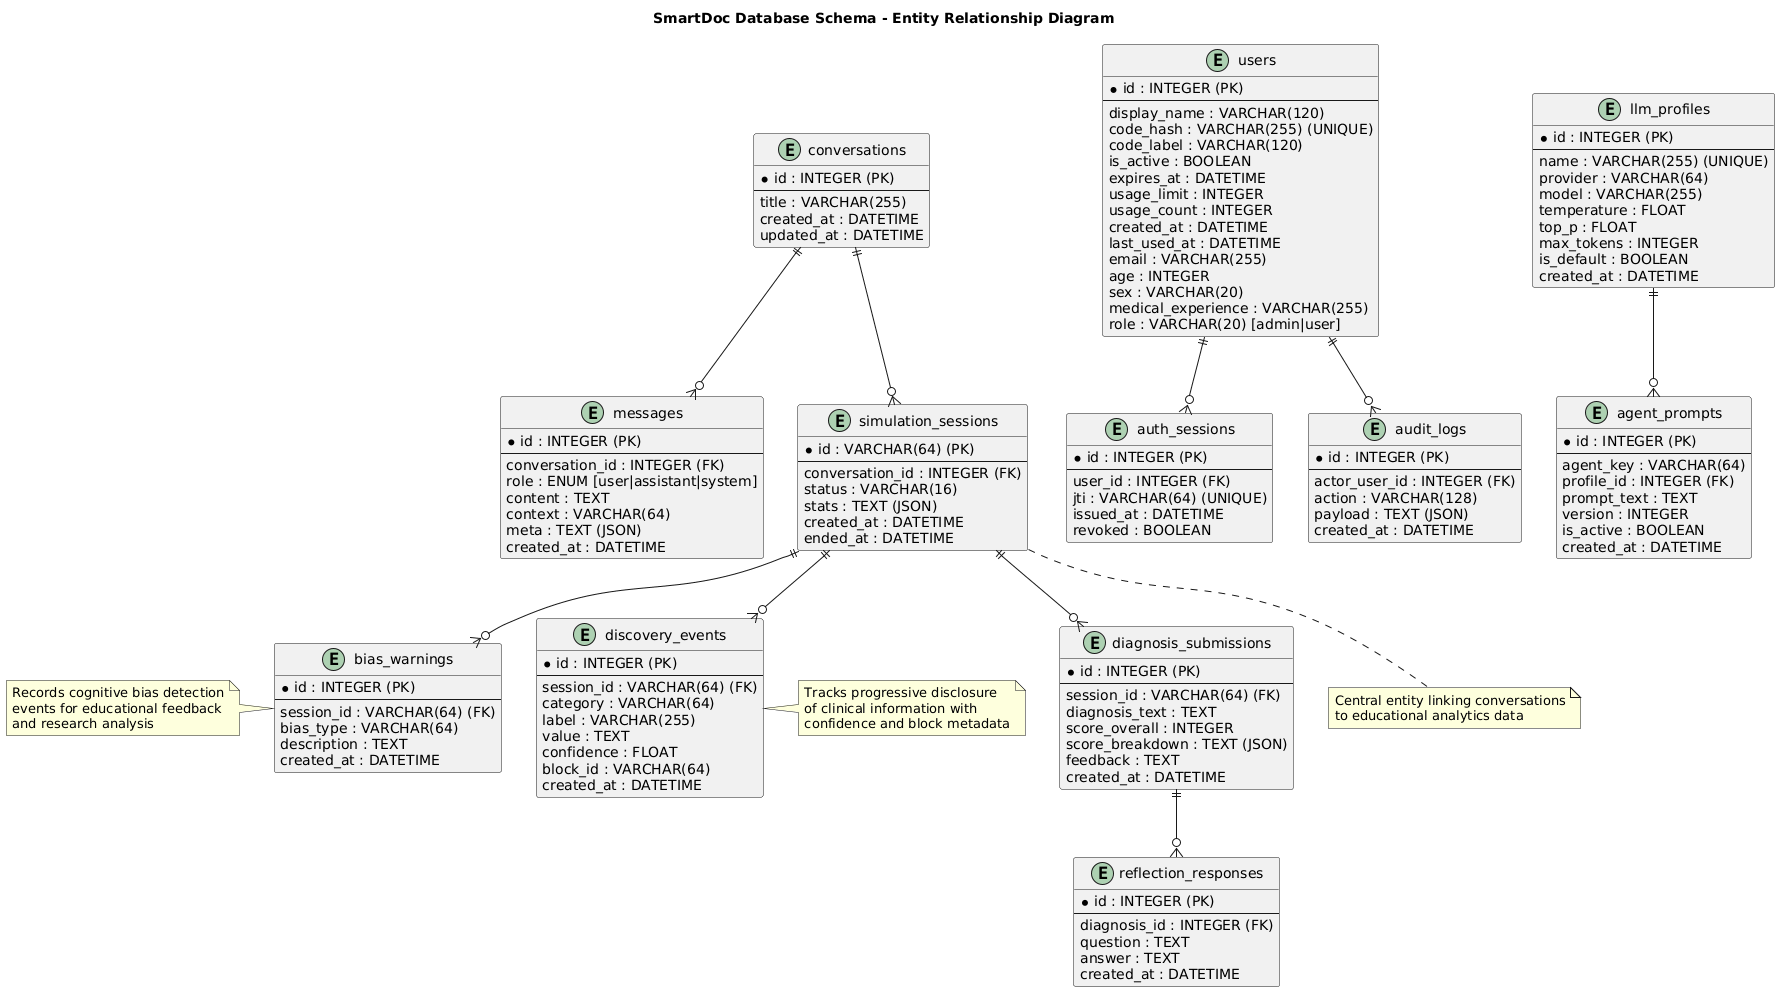
\includegraphics[width=0.82\textwidth]{figures/diagrams/erdb.png}
    \caption{Conceptual schema: capturing reasoning traces, bias events, and reflection data.}
    \label{fig:db_schema}
\end{figure}

\subsubsection{Session State and Event Hooks}

During an active simulation, a lightweight in-memory store maintains the
interaction-critical state. This keeps per-turn decisions fast while persisting
pedagogically relevant events to the database.

\noindent\textbf{Session state (simplified).}
\begin{verbatim}
class SessionState:
    session_id: str
    case_id: str
    current_phase: DiagnosticPhase   # anamnesis | exam | labs
    revealed_blocks: Set[str]        # information block IDs
    query_history: List[Query]       # learner queries with intents
    working_hypothesis: Optional[str]
    bias_warnings_triggered: List[BiasWarning]
    start_time: datetime
\end{verbatim}

\noindent\textbf{Event-driven persistence (illustrative).}
\begin{verbatim}
@on_reveal
def handle_information_revealed(block: InformationBlock):
    update_session_state(block)
    log_to_database(
        event="discovery",
        category=block.category,
        label=block.label,
        value=block.content,
        block_id=block.id,
        timestamp=now()
    )

@on_bias_detected
def handle_bias_detected(bias_type: str, description: str):
    issue_warning(bias_type)
    log_to_database(
        event="bias_warning",
        bias_type=bias_type,
        description=description,
        timestamp=now()
    )
\end{verbatim}

This event model ensures that (i) progressive disclosure decisions and
(ii) cognitive bias detections are both experienced by learners \emph{and}
captured for empirical study (see Chapter~\ref{chap:results}).

\subsubsection{Choice of Database Technology}

For research portability and reproducibility, SQLite was selected:
(i) single-file datasets simplify sharing and archiving;
(ii) no external service is required for classroom or multi-site pilots;
(iii) ACID guarantees protect integrity on abrupt termination;
(iv) identical environments are easy to reproduce. While SQLite is not intended
for heavy concurrent writes, SmartDoc’s usage pattern (individual or small-cohort
sessions) fits well. SQLAlchemy abstracts the backend, enabling future migration
to PostgreSQL/MySQL if needed.

\subsubsection{Logging for Reproducibility and Research}

Each session yields a complete, auditable reasoning trace.

\noindent\textbf{Interaction traces}
(timestamps for all items):
\begin{itemize}
  \item Learner queries, classified intents (with confidence and brief explanation).
  \item Information blocks revealed (sequence and dependencies).
  \item Responder outputs (anamnesis, exam, investigations).
\end{itemize}

\noindent\textbf{Pedagogical events}
\begin{itemize}
  \item Discovery events grouped by category (e.g., presenting\_symptoms, imaging).
  \item Bias warnings with type, timing, and triggering context.
  \item Reflection prompts and learner responses.
  \item Diagnosis submissions with full rubric breakdown and narrative feedback.
\end{itemize}

\noindent\textbf{Technical metrics}
\begin{itemize}
  \item LLM inference times and token counts.
  \item Classification confidence distributions.
  \item Fallback activations and recovery outcomes.
  \item Error types and handling paths.
\end{itemize}

These data support: (i) formative debriefs, (ii) summative assessment, and
(iii) research analytics (pattern mining, intervention evaluation), addressing
calls from the literature for transparent, empirically grounded evaluation.

\subsubsection{Worked Example: Excerpt from a Real Session}

\noindent\textit{Session:} \texttt{SESS\_0W451OZEJ} (\texttt{mull\_case}); compacted for brevity.
\begin{verbatim}
{
  "session_id": "SESS_0W451OZEJ",
  "conversation_id": 8,
  "messages": [
    {"id":153,"role":"user","content":"What is her past medical history?",
     "context":"anamnesis","meta":{"intent_id":"pmh_general","intent_confidence":0.95}},
    {"id":154,"role":"assistant","content":"Uh, she has morbid obesity, diabetes, ..."}
  ],
  "discoveries": [
    {"id":57,"category":"presenting_symptoms","label":"PMH",
     "value":"Morbid obesity, diabetes, hypertension, rheumatoid arthritis"}
  ],
  "bias_warnings": [
    {"id":3,"bias_type":"anchoring",
     "description":"Focus on cardiac hypothesis after preliminary CXR"}
  ],
  "diagnosis_submissions": [
    {"id":9,"diagnosis_text":"miliary tuberculosis",
     "score_overall":81,
     "score_breakdown":{"information_gathering":75,"diagnostic_accuracy":88,
                        "cognitive_bias_awareness":80}}
  ],
  "statistics": {
    "total_messages": 34,
    "session_duration_minutes": 20.7
  }
}
\end{verbatim}

\subsubsection{Privacy and Security Considerations}

Although SmartDoc is a research prototype, data-protection principles were
embedded from the outset:

\begin{itemize}
  \item \textbf{Access control:} role-based authentication; learners can only view their
        own sessions; instructors access aggregated analytics.
  \item \textbf{Data minimisation:} simulated cases only; no real patient data or
        personally identifiable medical information.

  \item \textbf{Local-first processing:} all data and LLM inference run locally;
        no external transmission; encrypted backups at rest.
\end{itemize}

This architecture supports responsive teaching while producing transparent,
reproducible research artefacts.

\subsection{Deployment Configuration and Scalability}
\label{sec:deploy}

SmartDoc was engineered to run reliably in both research and teaching contexts. The deployment architecture follows three principles: (i) \emph{reproducibility} across sites and machines, (ii) \emph{scalability} for cohort use, and (iii) \emph{accessibility} via lightweight, low-ops setups.

\subsubsection{Containerised Services}
For consistent behaviour across environments, SmartDoc is packaged as Docker services: a Flask/Gunicorn web application, a local LLM inference service (Ollama), and a persistent database volume. This encapsulation ensures pinned dependencies and enables single-command bring-up for workshops and classes.

\noindent\textbf{Service roles (concise).}
\begin{itemize}
  \item \textbf{Web application} (Flask + Gunicorn): HTTP API, static files, request concurrency.
  \item \textbf{LLM inference} (Ollama): local hosting of the selected model; optional GPU.
  \item \textbf{Database} (SQLite): ACID single-file store for reasoning traces and analytics.
  \item \textbf{Logging} (structured JSON): access, error, and audit logs with daily rotation.
\end{itemize}

Full container definitions and startup scripts (model preload, migrations) are listed in Appendix~\ref{app:ops}, enabling exact replication without cluttering the main text.

\subsubsection{Model Hosting Modes}
SmartDoc supports two deployment modes to accommodate institutional constraints:

\paragraph{Local hosting (privacy and research).}
Ollama serves a quantised open model locally. Advantages: data stays on-prem, fixed model versioning for reproducibility, no API cost; limitations: modest hardware needs (8\,GB+ RAM; GPU recommended) and lower raw accuracy than premium APIs.

\paragraph{Cloud APIs (scale and convenience).}
The provider abstraction can target commercial models for large courses. Advantages: managed scaling and state-of-the-art quality; trade-offs: per-call cost, external data processing, and behaviour shifts with upstream updates.

This dual-mode design lets programmes choose the balance between cost, accuracy, and governance.

\subsubsection{Scaling Strategy}
Although most learners interact individually, classroom use requires concurrency. We scale at three layers:

\paragraph{Application tier.}
Multiple Gunicorn workers per container, and (optionally) multiple app replicas behind a lightweight load balancer, increase request throughput without code changes.

\paragraph{Inference tier.}
For local deployments, multiple Ollama instances can be load-balanced to reduce queueing under peak load. In cloud mode, provider-side autoscaling handles bursty traffic.

\paragraph{Data tier.}
SQLite is adequate up to small cohorts with modest write contention. The SQLAlchemy layer allows a drop-in migration to PostgreSQL for larger installations requiring high concurrency and centralised logging.

\subsubsection{Persistence and Observability}
Two volumes persist the database and logs across restarts. Operational logs (request timings, inference latency, classification confidences, and error traces) are emitted in structured JSON to enable programmatic monitoring and bottleneck diagnosis.

\subsubsection{Educational Implications}
By prioritising reproducibility and portability, institutions can deploy SmartDoc with minimal operational overhead (\texttt{docker compose up}) in labs, classrooms, or research pilots. The combination of (i) local, privacy-preserving hosting and (ii) an optional cloud path for scale turns deployment choices into \emph{educational enablers}: instructors retain immersion (low perceived latency), researchers can replicate analyses exactly, and learners benefit from dependable access in varied settings.

\section{Example Workflow: The Miliary Tuberculosis Case}
\label{sec:mtb_workflow}

This section illustrates a complete diagnostic workflow in SmartDoc using real session data. The case demonstrates how intent classification, progressive disclosure, educational scaffolding, bias detection, and metacognitive evaluation work together in practice.

\subsection{Case Overview and Educational Objectives}

The case adapts Mull et~al.'s\cite{mull_cognitive_2015} published example of diagnostic error, in which an elderly Spanish-speaking woman with dyspnoea was repeatedly misdiagnosed with heart failure due to cognitive biases. SmartDoc converts this report into an interactive experience that makes bias tangible and addressable.

\textbf{Note:} The following workflow is a compact version of the full transcript . Readers can see the full transcript with all the respective data in Apendix C  \ref{app:session_s6}

\noindent\textbf{Initial presentation}
\begin{quote}
``A Spanish speaker 85-year-old woman presents with worsening shortness of breath over 2~months. Her son provides the history..''
\end{quote}

\noindent\textbf{Educational objectives}
\begin{enumerate}
  \item Practise systematic information gathering across history, examination, and investigations.
  \item Demonstrate medication reconciliation in complex patients.
  \item Integrate contradictory evidence (normal echo vs.\ elevated BNP).
  \item Identify the critical diagnostic clue (immunosuppressant use).
\end{enumerate}

\noindent\textbf{Correct diagnosis:} Miliary tuberculosis secondary to TNF-$\alpha$ inhibitor therapy. \\
\textbf{Common misdiagnosis:} Acute heart failure exacerbation (anchoring trap).

\subsection{Phase-by-Phase Walkthrough}

\paragraph{Phase~1: Anamnesis (Interactions~1--10; \(\sim\)7~min)}
\textit{Interaction 1 --- Past medical history} \\
Student: ``First, what is her past medical history?'' \\
Intent: \texttt{pmh\_general} (conf.~0.95) \\
Son: ``Uh, she has a history of morbid obesity, diabetes, hypertension, and rheumatoid arthritis.'' \\
\emph{Discovery:} \texttt{pmh\_comorbidities} (presenting\_symptoms).

\smallskip
\textit{Interaction 2 --- Chief complaint} \\
Student: ``And what brings you here today?'' \\
Intent: \texttt{hpi\_chief\_complaint} (conf.~0.95) \\
Son: ``Trouble breathing on exertion, dry cough.'' \\
\emph{Discovery:} \texttt{hpi\_dyspnea\_details}.

\smallskip
\textit{Interaction 3 --- Duration} \\
Student: ``For how long is she having trouble breathing?'' \\
Intent: \texttt{hpi\_onset\_duration\_primary} (conf.~0.95) \\
Son: ``Gradually worsening for about two months.'' \\
\emph{Discovery:} \texttt{hpi\_onset\_duration}. \\
\emph{Note:} The subacute timeline argues against acute cardiac decompensation.

\smallskip
\textit{Interaction 4 --- Current medications} \\
Student: ``Any regular medication?'' \\
Intent: \texttt{meds\_current\_known} (conf.~0.95) \\
Son: ``Lisinopril, atenolol, glipizide, metformin---I think.'' \\
\emph{Discovery:} \texttt{meds\_initial\_known} (Level~1). \\
\emph{Signal:} Family uncertainty foreshadows the need for deeper reconciliation.

\smallskip
\textit{Interaction 5 (critical) --- RA medications (first attempt)} \\
Student: ``Is she taking anything for her rheumatoid arthritis?'' \\
Intent: \texttt{meds\_ra\_specific\_initial\_query} (conf.~0.98) \\
Son: ``I'm not sure, sorry.'' \\
\emph{Discovery:} \texttt{meds\_ra\_uncertainty} (Level~2). \\
\emph{Pedagogy:} Productive friction; tests learner persistence.

\smallskip
\textit{Interactions 6--8 --- Constitutional \& chest symptoms} \\
Fevers? (No), night chills? (No), chest pain? (No). \\
\emph{Discoveries:} three pertinent negatives.

\paragraph{Phase~2: Physical examination (Interactions~9--11; \(\sim\)3~min)}
\textit{Interaction 9 --- Vital signs} \\
Intent: \texttt{exam\_vital} (conf.~0.95) \\
System: Temp~99.9$^\circ$F, HR~105, BP~140/70, RR~24, O$_2$~sat~89\% (RA). \\
\emph{Discovery:} \texttt{exam\_vital}.

\smallskip
\textit{Interaction 10 --- Cardiac examination} \\
Intent: \texttt{exam\_cardiovascular} (conf.~0.98) \\
System: Normal heart sounds, no leg oedema. \\
\emph{Discovery:} \texttt{exam\_cardiac\_negative}. \\
\emph{Signal:} Contradictory to heart failure.

\smallskip
\textit{Interaction 11 --- Pulmonary examination} \\
Intent: \texttt{exam\_respiratory} (conf.~0.98) \\
System: Crackles in all lung fields. \\
\emph{Discovery:} \texttt{exam\_respiratory}.

\paragraph{Phase~3: Investigations (Interactions~12--17; \(\sim\)8~min)}
\textit{Interaction 12 (anchoring trap) --- Chest X-ray} \\
Intent: \texttt{imaging\_chest\_xray} (conf.~0.95) \\
System: Preliminary read: ``pulmonary vascular congestion''. \\
\emph{Discovery:} \texttt{imaging\_cxr\_preliminary}. \\
\emph{Bias trigger:} Anchoring towards heart failure (warning logged).

\smallskip
\textit{Interaction 13 --- RA meds (second attempt) + scaffold} \\
Intent: \texttt{meds\_ra\_specific\_initial\_query} (conf.~0.95) \\
Hint injected: ``Maybe you could check previous hospital records?''

\smallskip
\textit{Interaction 14 (critical) --- Full reconciliation success} \\
Intent: \texttt{meds\_full\_reconciliation\_query} (conf.~0.98) \\
Son: ``She was receiving \emph{infliximab} for rheumatoid arthritis.'' \\
\emph{Discovery:} \texttt{critical\_infliximab} (Level~3, critical).

\smallskip
\textit{Interaction 15 --- Chest CT} \\
Intent: \texttt{imaging\_ct\_chest} (conf.~0.95) \\
System: Reticular pattern with innumerable 1--2\,mm nodules (miliary). \\
\emph{Discovery:} \texttt{critical\_ct\_chest} (critical).

\smallskip
\textit{Interaction 16 --- Bloodwork} \\
Intent: \texttt{labs\_general} (conf.~0.95) \\
System: Elevated pro-BNP; WBC~13.0\,$\times 10^9$/L; Hb~10\,g/dL. \\
\emph{Discoveries:} \texttt{labs\_bnp}, \texttt{labs\_wbc}, \texttt{labs\_hemoglobin}. \\
\emph{Signal:} BNP is a red herring; leukocytosis supports infection/inflammation.

\smallskip
\textit{Interaction 17 (contradictory) --- Echocardiogram} \\
Intent: \texttt{imaging\_echo} (conf.~0.95) \\
System: Normal EF; no elevated filling pressures. \\
\emph{Discovery:} \texttt{critical\_echo} (contradicts heart failure).

\subsection{Summary of Information Revealed}

\begin{table}[h]
\centering
\caption{Discoveries by category and timing.}
\label{tab:discoveries_mtb}
\begin{tabular}{lccc}
\toprule
\textbf{Category} & \textbf{Count} & \textbf{Critical Findings} & \textbf{Timeline} \\
\midrule
Presenting symptoms   & 6 & None                             & First 2 min \\
Current medications   & 3 & Infliximab        & min~\(\sim 7\) \\
Physical examination  & 3 & None                             & 7--10 min \\
Imaging               & 3 & Miliary nodules; normal echo     & 10--15 min \\
Diagnostic results    & 3 & None            & 15--18 min \\
\midrule
\textbf{Total}        & \textbf{18} & \textbf{2 critical}        & \textbf{18 min} \\
\bottomrule
\end{tabular}
\end{table}

\subsection{Diagnosis and Reflection}

\noindent\textbf{Submitted diagnosis:} ``miliary tuberculosis''

\smallskip
\noindent\textbf{Reflection (excerpts).}
\begin{itemize}
  \item \emph{Most compelling evidence:} Chest CT with diffuse 1--2\,mm nodules plus recent infliximab (TNF-$\alpha$ inhibition) \(\rightarrow\) classic for miliary TB.
  \item \emph{Evidence against:} Elevated BNP and crackles are nonspecific; absence of oedema and normal cardiac exam argue against cardiac aetiology.
  \item \emph{Alternatives:} Acute heart failure exacerbation; interstitial lung disease (RA/drug toxicity).
  \item \emph{Ruling alternatives:} Normal EF and filling pressures on echo effectively rule out acute heart failure.
  \item \emph{Must-not-miss considered:} Pulmonary embolism, severe pneumonia, acute heart failure---systematically deprioritised based on course and imaging pattern.
\end{itemize}

\subsection{Evaluation Results}

\noindent\textbf{Overall:} 81/100 \\
\textbf{Information gathering:} 75/100 \quad
\textbf{Diagnostic accuracy:} 88/100 \quad
\textbf{Cognitive bias awareness:} 80/100

\smallskip
\noindent\textbf{Strengths.} Correct diagnosis; avoided HF trap; recognised infliximab risk; integrated contradictory evidence; reasonable differential. \\
\textbf{Areas to improve.} More explicit documentation of weight loss/constitutional features; deeper analysis of anchoring; concrete prevention strategies for future cases. \\
\textbf{Key recommendation.} Adopt a structured medication-reconciliation checklist with explicit prompts for immunosuppressants/biologics; actively challenge preliminary imaging reads.

\subsection{Educational Impact Analysis}

\paragraph{Progressive disclosure}
The learner revealed 18 information blocks via 17 queries, evidencing active inquiry. Medication reconciliation required semantic precision (Level~1\,\(\rightarrow\)\,Level~3).

\paragraph{Scaffolding effectiveness}
A single just-in-time hint after repeated RA-medication queries led to successful escalation and discovery of the infliximab clue.

\paragraph{Bias demonstration}
The preliminary CXR created an anchoring opportunity; a warning was logged when cardiac focus persisted. Subsequent CT and echo helped the learner de-anchor.

\paragraph{Metacognition}
Reflections showed explicit evidence integration (infliximab\,\(\rightarrow\)\,TB), acknowledgement of contradictions (normal echo vs.\ BNP), plausible alternatives, and reasoning about rule-in/out steps.

\paragraph{System performance}
Intent classification accuracy was high (17/17 correct). End-to-end response latency in this session was \(\sim 6\)~seconds per turn (consistent with Chapter~\ref{chap:results}); model-only generation is faster but network/ui overheads dominate in practice. The educational hint deployed once (effective), and one anchoring warning was appropriately triggered.

\section{User Interfaces}
\label{sec:ui}

SmartDoc's user-facing components translate the technical architecture into accessible, pedagogically effective interfaces. The design philosophy prioritizes \textbf{cognitive focus} over visual complexity—students should concentrate on clinical reasoning rather than navigating complex software. This section describes the two primary interfaces: the simulation environment for students and the administrative dashboard for educators.

\subsection{Simulation Interface}
\label{subsec:ui-sim}

The simulation interface presents as a single-page web application accessible through any modern browser. The design deliberately avoids medical record system mimicry, instead providing a clean, distraction-free environment that foregrounds diagnostic thinking.

\subsubsection*{Layout and Core Components}

\paragraph{Four-Tab Organization}

\begin{figure}[h]
  \centering
  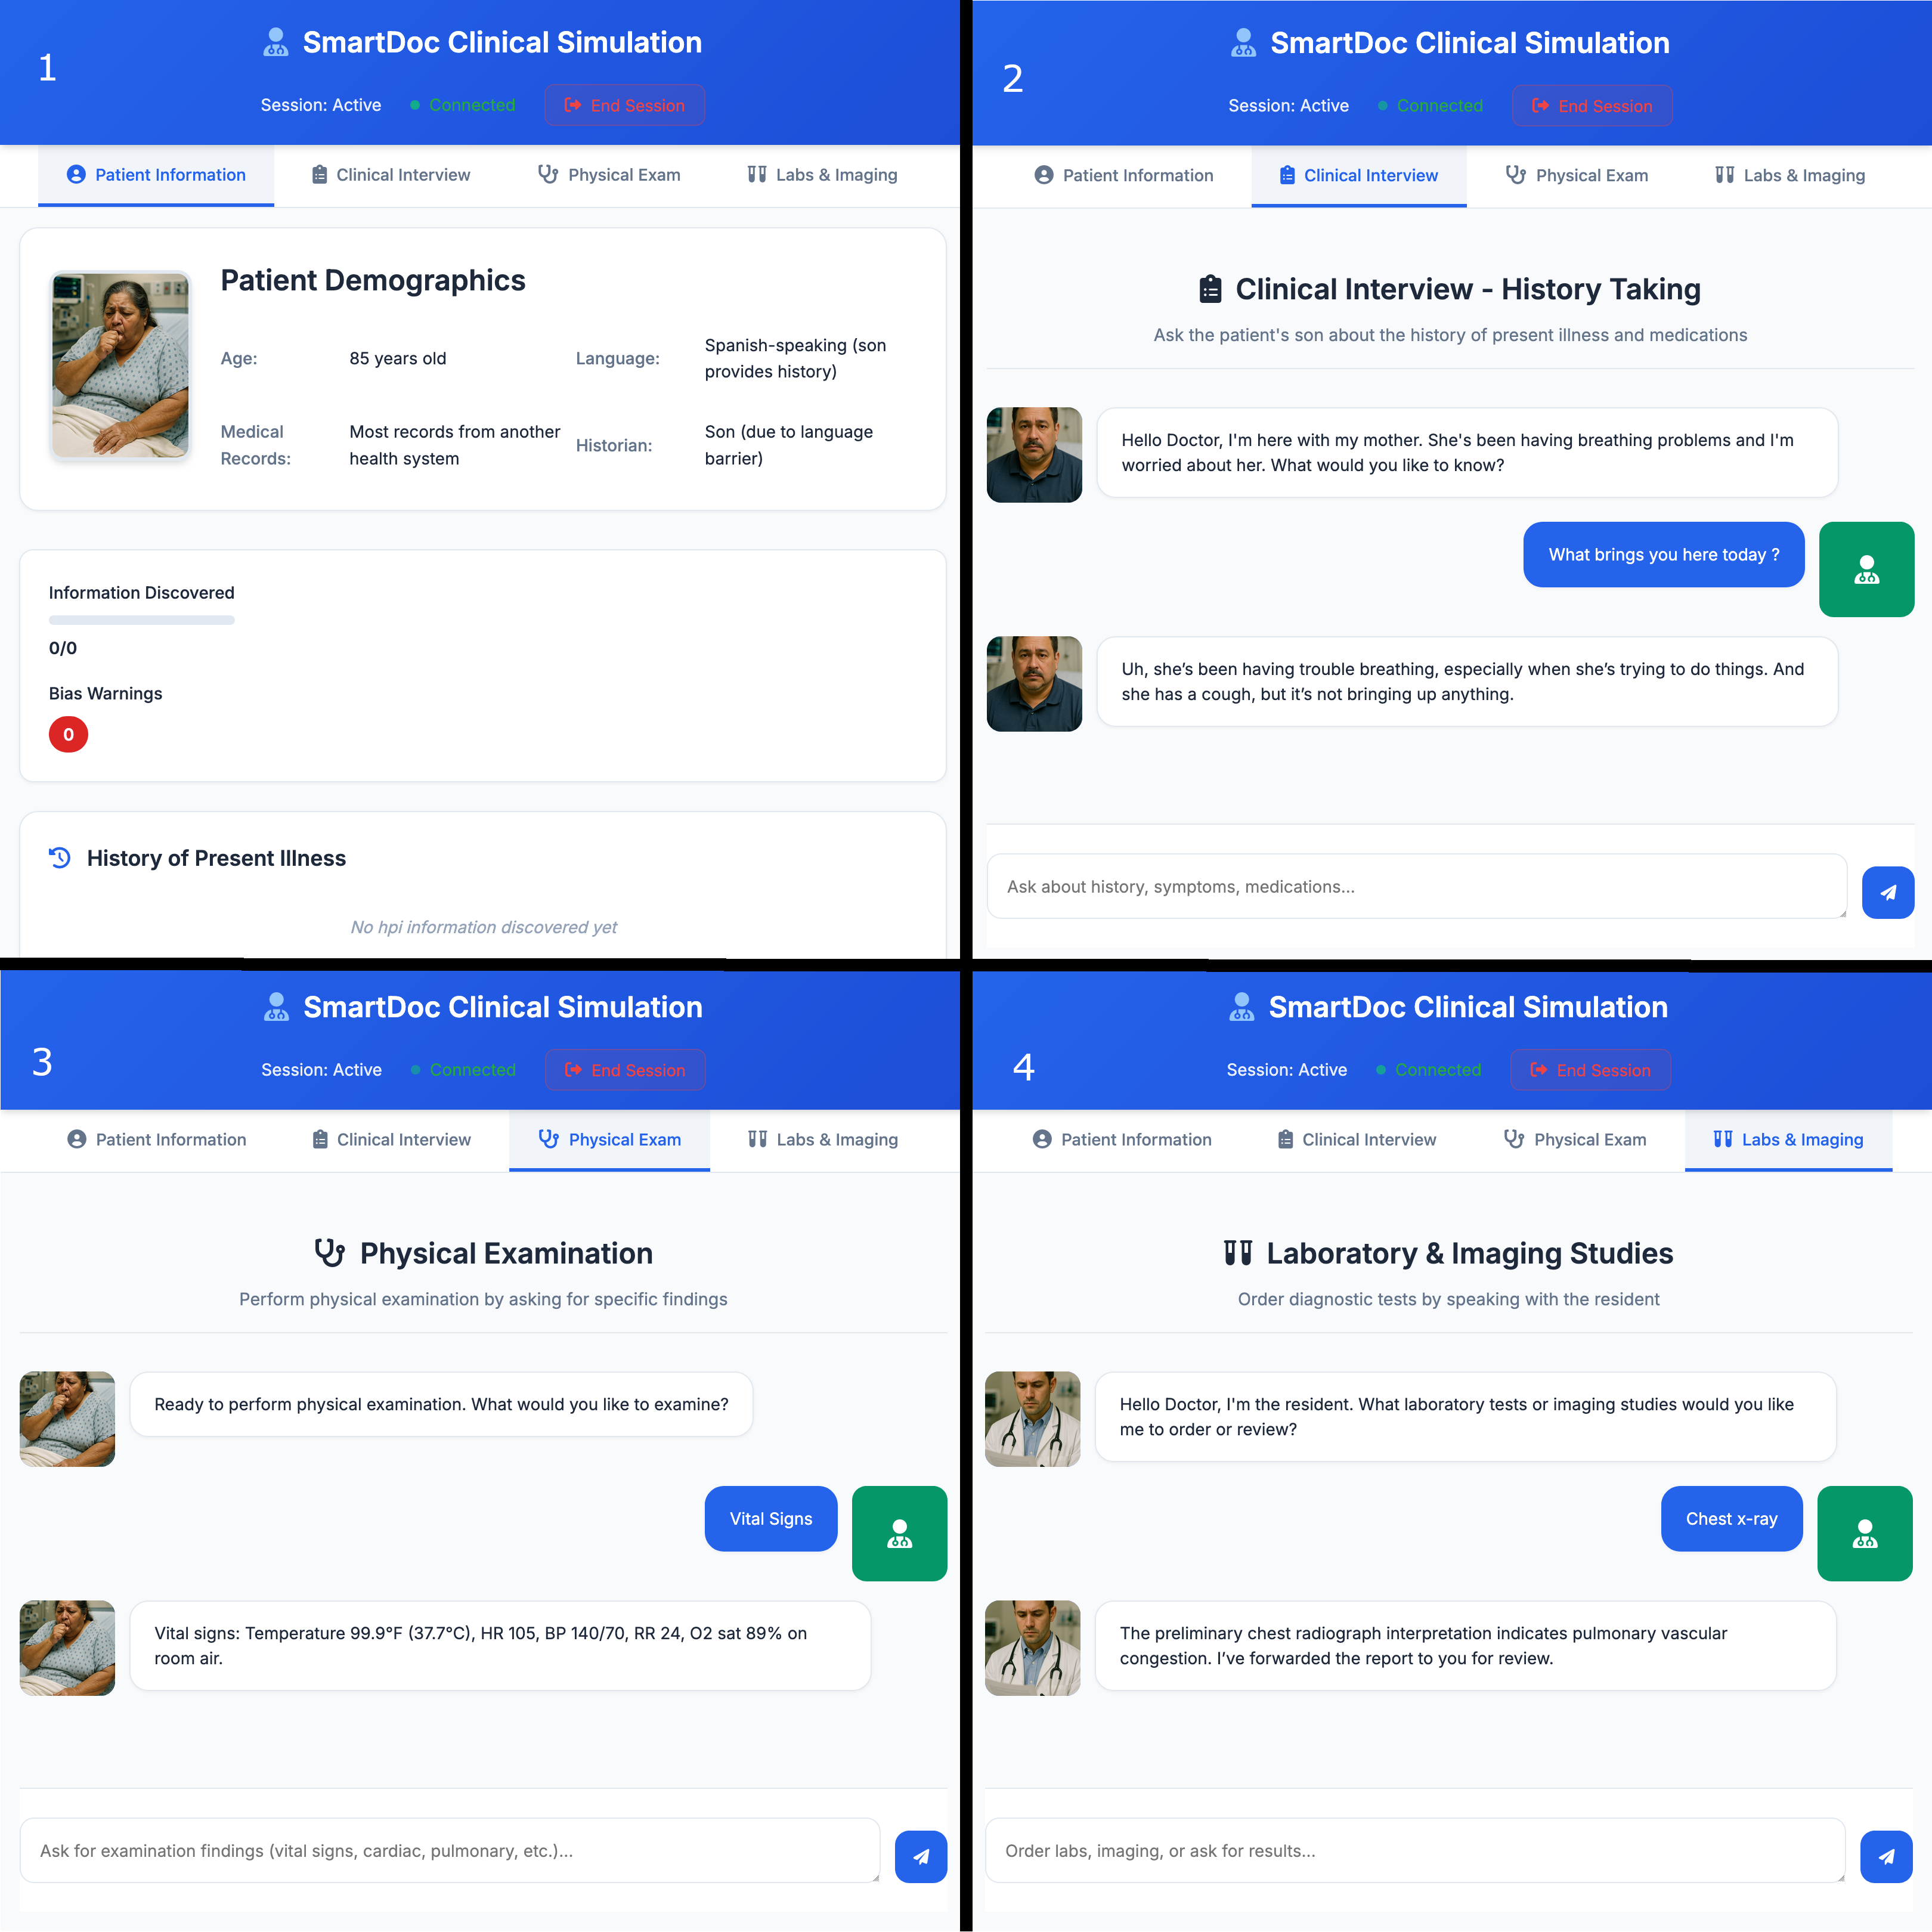
\includegraphics[width=0.95\textwidth]{figures/ui/ui_layout_overview.png}
  \caption{Simulation interface: four-tab layout (1- Patient Information, 2- Clinical Interview, 3- Physical Exam, 4- Labs \& Imaging).}
  \label{fig:ui-layout}
\end{figure}

\begin{enumerate}
  \item \textbf{Patient Information tab}
  \begin{itemize}
    \item Basic demographics and presenting context
    \item Information and bias live counter.
    \item List of revealed information organized by category
    \item Diagnosis submission form.
  \end{itemize}

  \item \textbf{Clinical Interview (anamnesis) Tab}
  \begin{itemize}
    \item Chat-based conversation with the patient's son
    \item Scrollable conversation history with visual distinction between user queries (right-aligned, blue) and system responses (left-aligned, gray)
  \end{itemize}

  \item \textbf{Physical Exam Tab}
  \begin{itemize}
    \item Chat-based physical objective exams requests to patient.
    \item Scrollable conversation history with visual distinction between user queries (right-aligned, blue) and system responses (left-aligned, gray)
  \end{itemize}


  \item \textbf{Labs \& Imaging}
  \begin{itemize}
    \item Chat-based conversation with the local resident to request imaging and lab exams.
    \item Scrollable conversation history with visual distinction between user queries (right-aligned, blue) and system responses (left-aligned, gray)
  \end{itemize}
\end{enumerate}


\paragraph{Revealed information blocks}

Below the patient demographics, revealed information blocks are organized into four categories.

\begin{figure}[h]
  \centering
  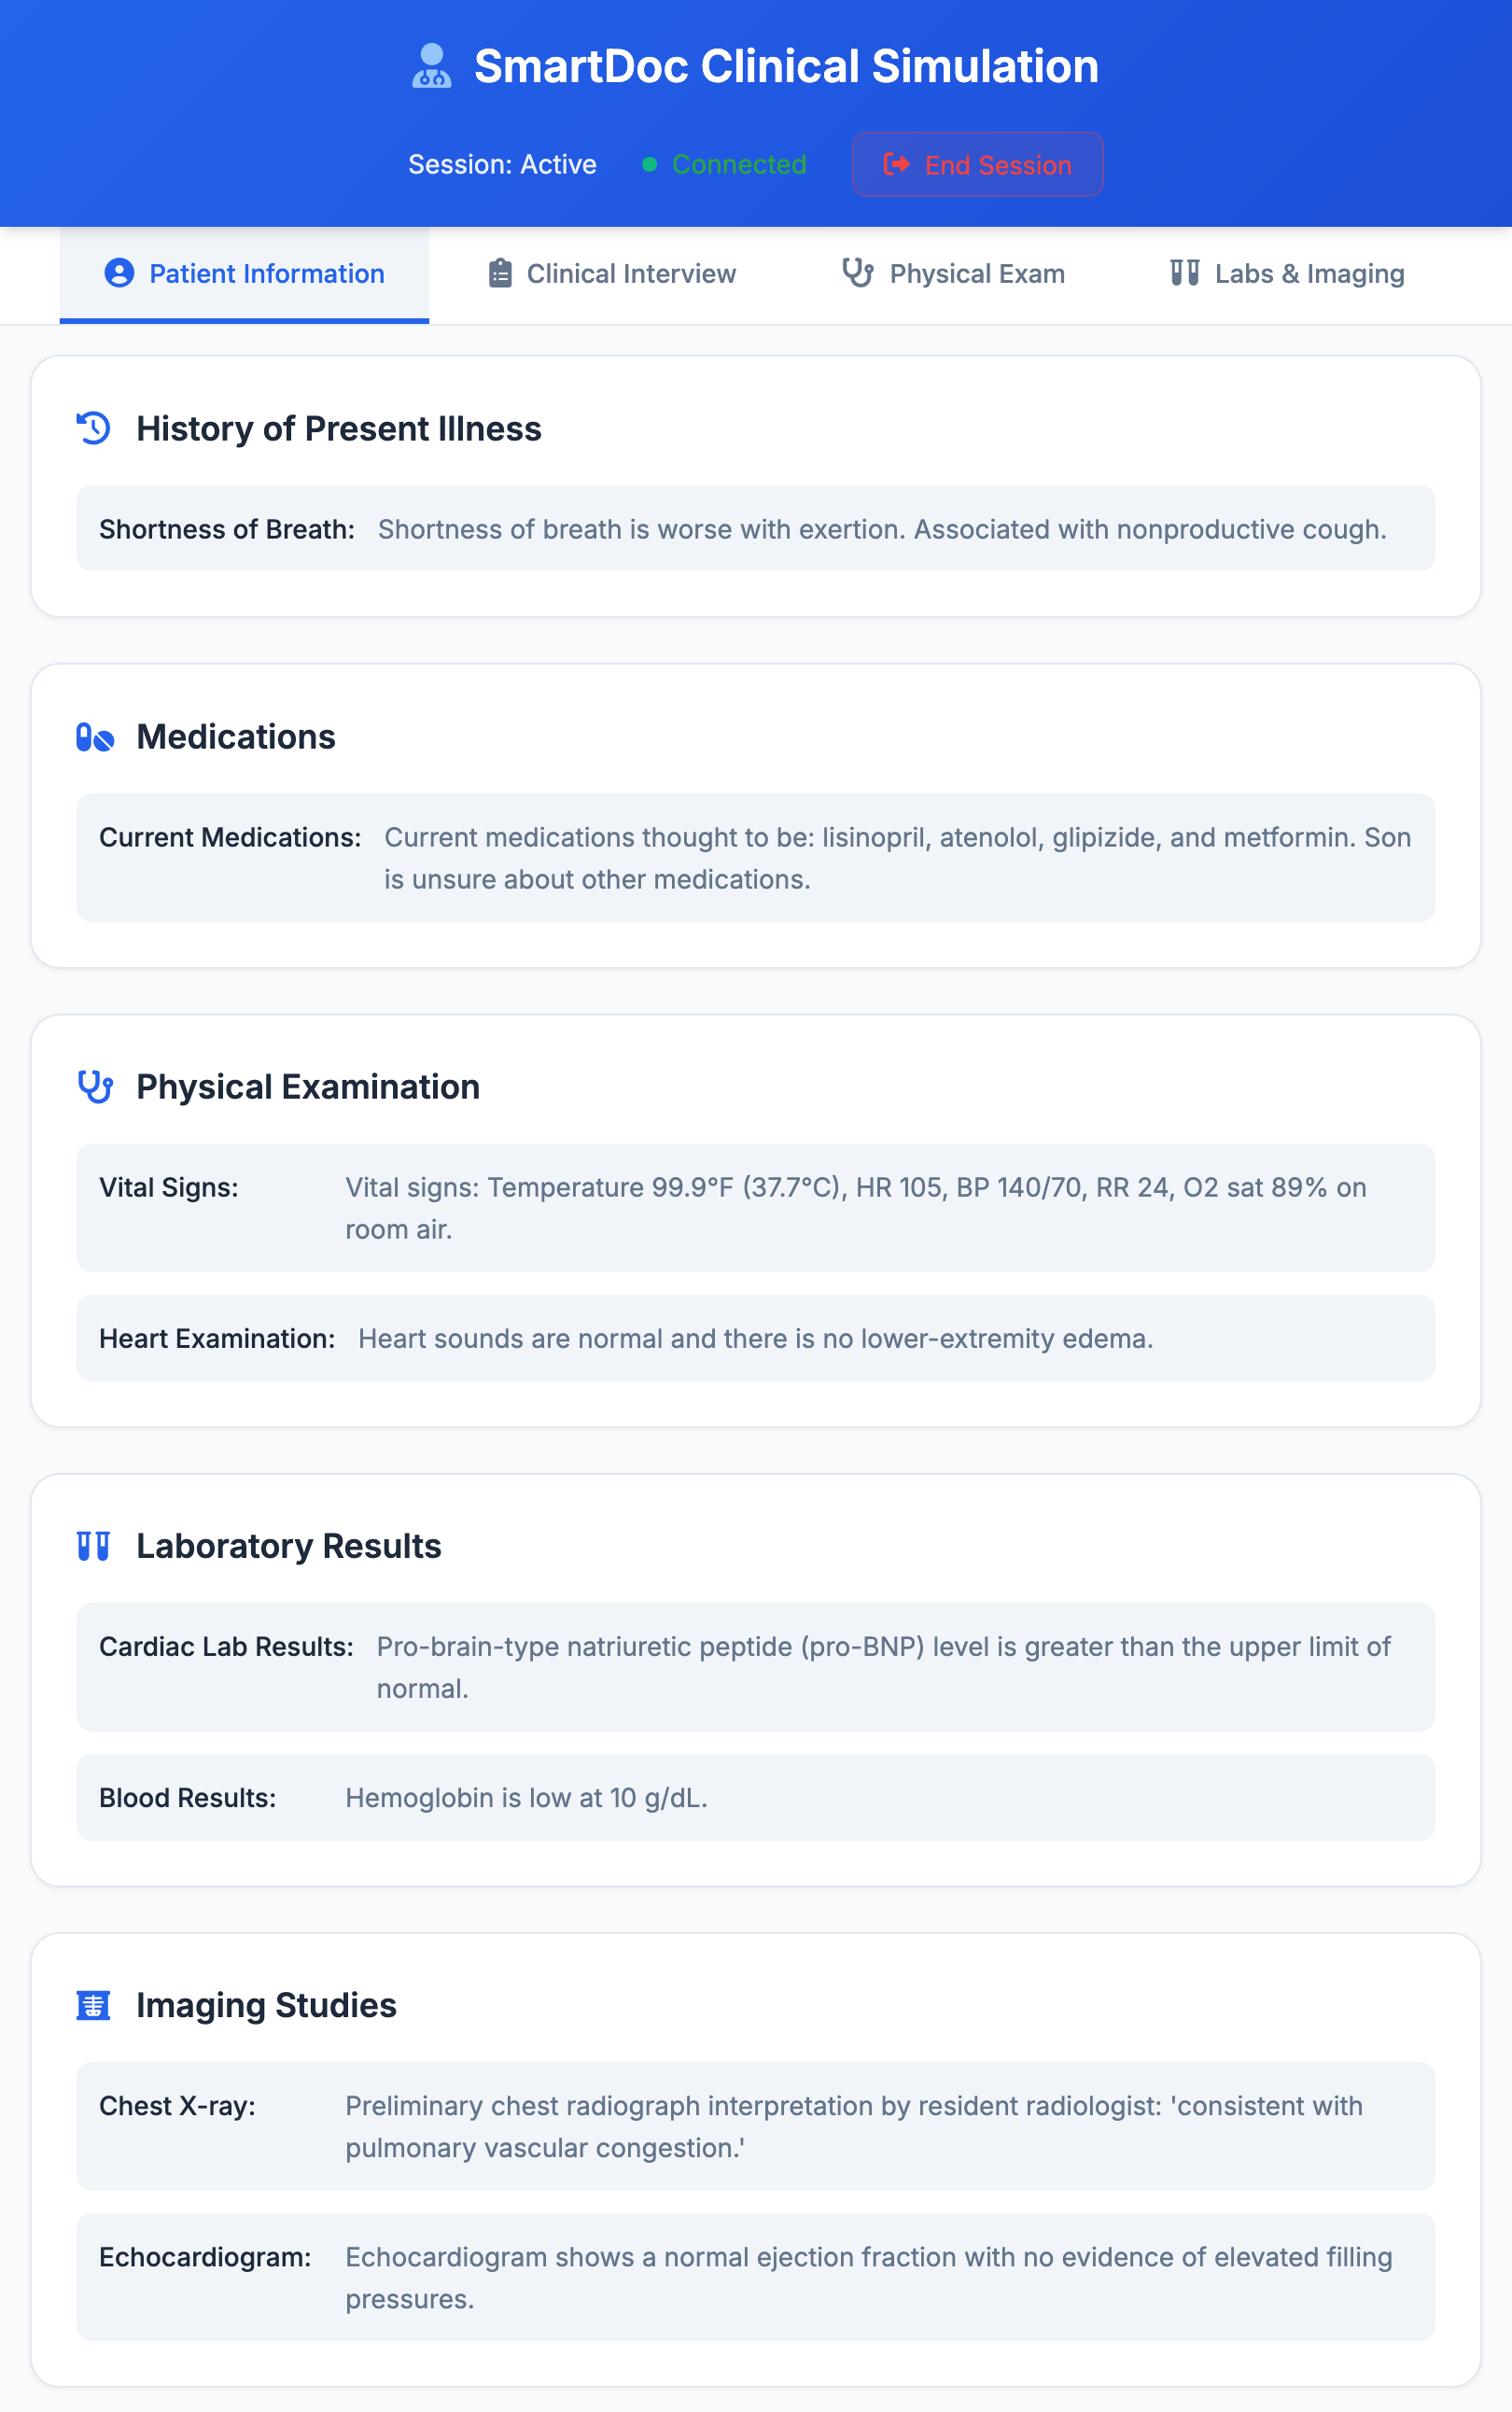
\includegraphics[width=0.5\textwidth]{figures/ui/ui_tabs_anamnesis_exam_results.png}
  \caption{Listed discovered blocks of information.}
  \label{fig:ui-tabs}
\end{figure}

\textit{Categories}
\begin{itemize}
  \item History of Present Illness
  \item Medications
  \item Physical Examination
  \item Laboratory Results
  \item Imaging studies
\end{itemize}
Each piece of information appears only after the student asks the relevant question.


\paragraph{Bias Warning Display}

When the bias detection system identifies a concerning pattern, a \textbf{bias warning card} appears in the active conversation tab.

\begin{figure}[h]
  \centering
  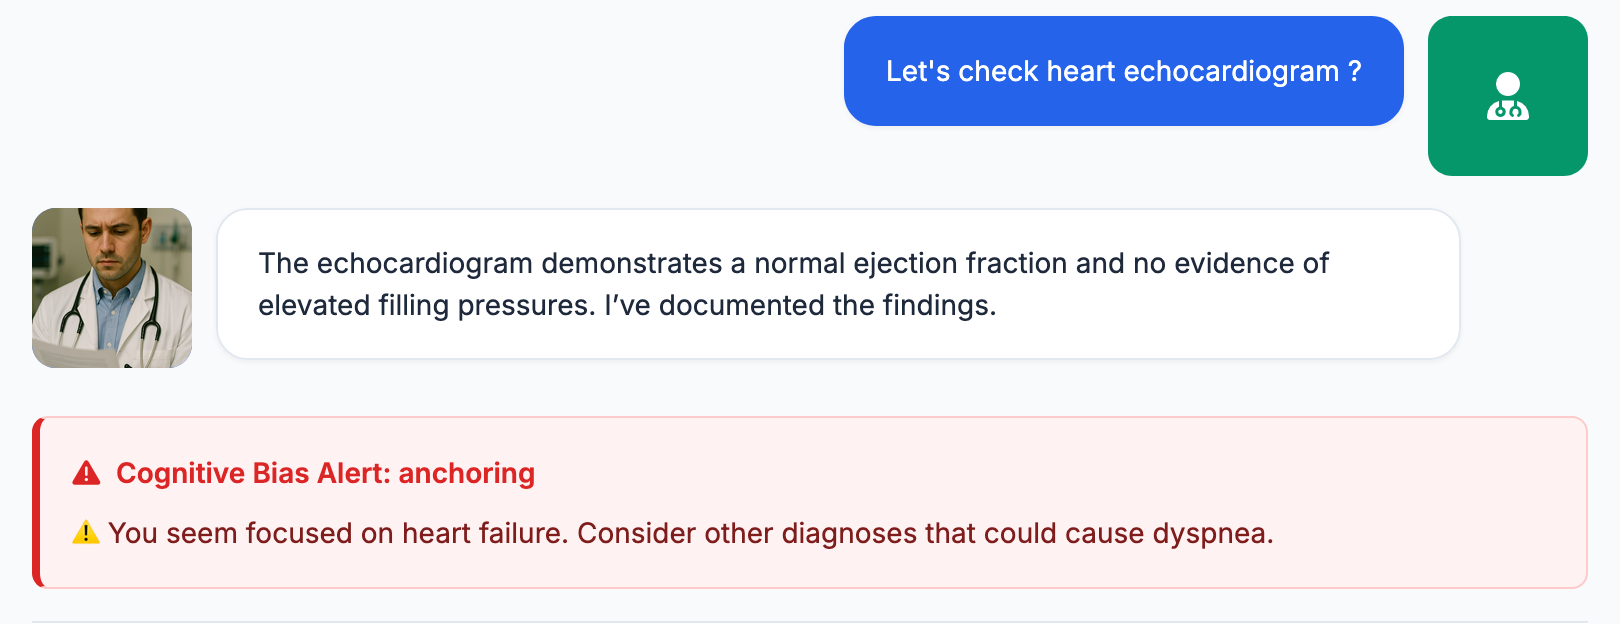
\includegraphics[width=0.75\textwidth]{figures/ui/ui_bias_card.png}
  \caption{Bias warning card (persistent, non-blocking) shown in the Discovery Panel.}
  \label{fig:ui-bias-card}
\end{figure}

The warning remains visible but non-blocking—students can continue investigating without dismissing it. This design choice reflects the pedagogical goal of making bias awareness metacognitively salient without punishing learners or creating frustration.

\paragraph{Diagnosis Submission Interface}

When the student feels ready to conclude the case, clicking ``Submit Diagnosis'' reveals a structured form with five metacognitive prompts

\begin{enumerate}
  \item \textbf{Submit Diagnosis} \\
  Free text, allowing students to write the diagnosis.
  \item \textbf{What is the single most compelling piece of evidence that supports your chosen diagnosis? } \\
  Forces explicit articulation of reasoning, preventing ``gut feeling'' diagnoses.
  \item \textbf{What evidence argues against your diagnosis?} \\
  Prompts consideration of contradictory data, engaging System~2 deliberation.
  \item \textbf{What else could this be? List at least two reasonable alternative diagnoses. } \\ 
  Assesses the breadth of differential diagnosis and systematic thinking. 
  \item \textbf{For one of your alternative diagnoses, what specific information (test or question) would help rule it in or out?} \\
  Evaluates understanding of diagnostic test characteristics and clinical decision-making.
  \item \textbf{Have you considered and ruled out any potential 'must-not-miss' or life-threatening conditions?} \\
  Evaluates understanding of structured anamnesis and reasoning.
\end{enumerate}

\begin{figure}[h]
  \centering
  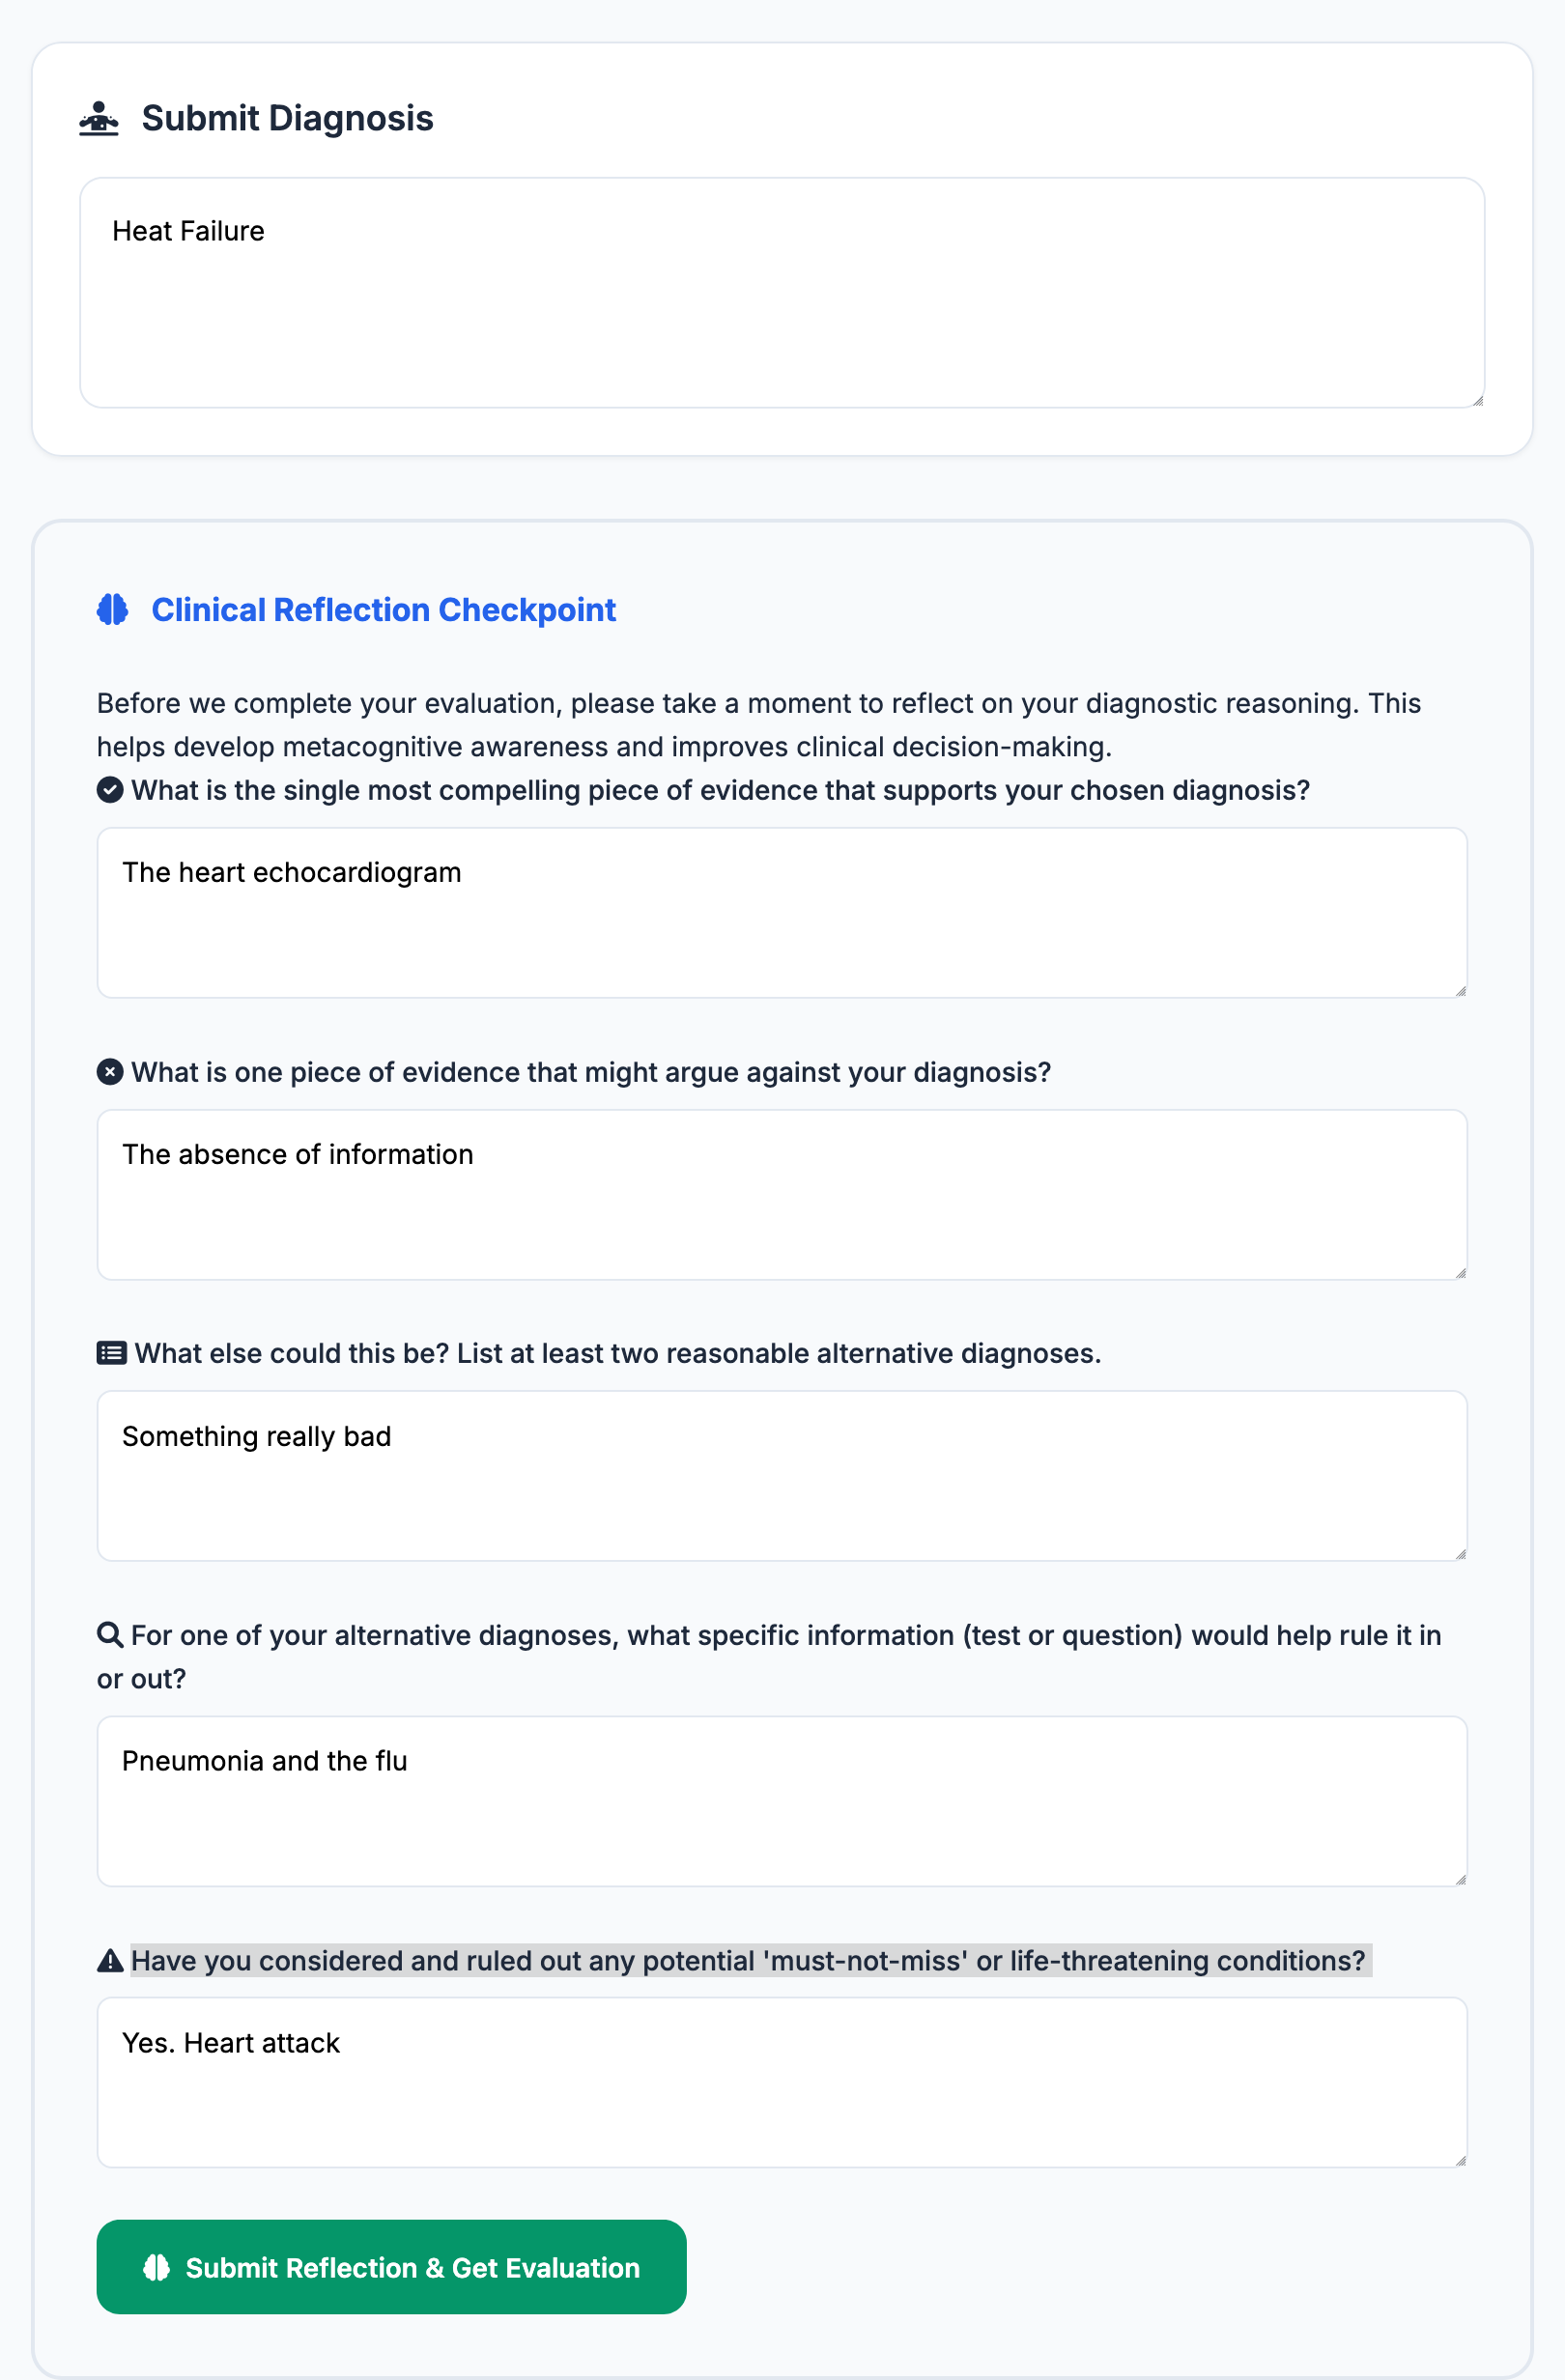
\includegraphics[width=0.7\textwidth]{figures/ui/ui_diagnosis_reflection.png}
  \caption{Diagnosis and reflection submission}
  \label{fig:ui-submission}
\end{figure}

Upon submission, the interface transitions to the evaluation results view.

\subsection{Evaluation Results Interface}
\label{subsec:ui-results}

After submission of the diagnosis, students receive extensive feedback organized into three sections.

\paragraph{Overall Performance Summary}
A prominent score display shows:
\begin{itemize}
  \item \textbf{Overall Score:} Number 0-100
  \item \textbf{Dimensional Breakdown:} Three sub-scores for Information Gathering, Diagnostic Accuracy, and Cognitive Bias Awareness
\end{itemize}

\begin{figure}[h]
  \centering
  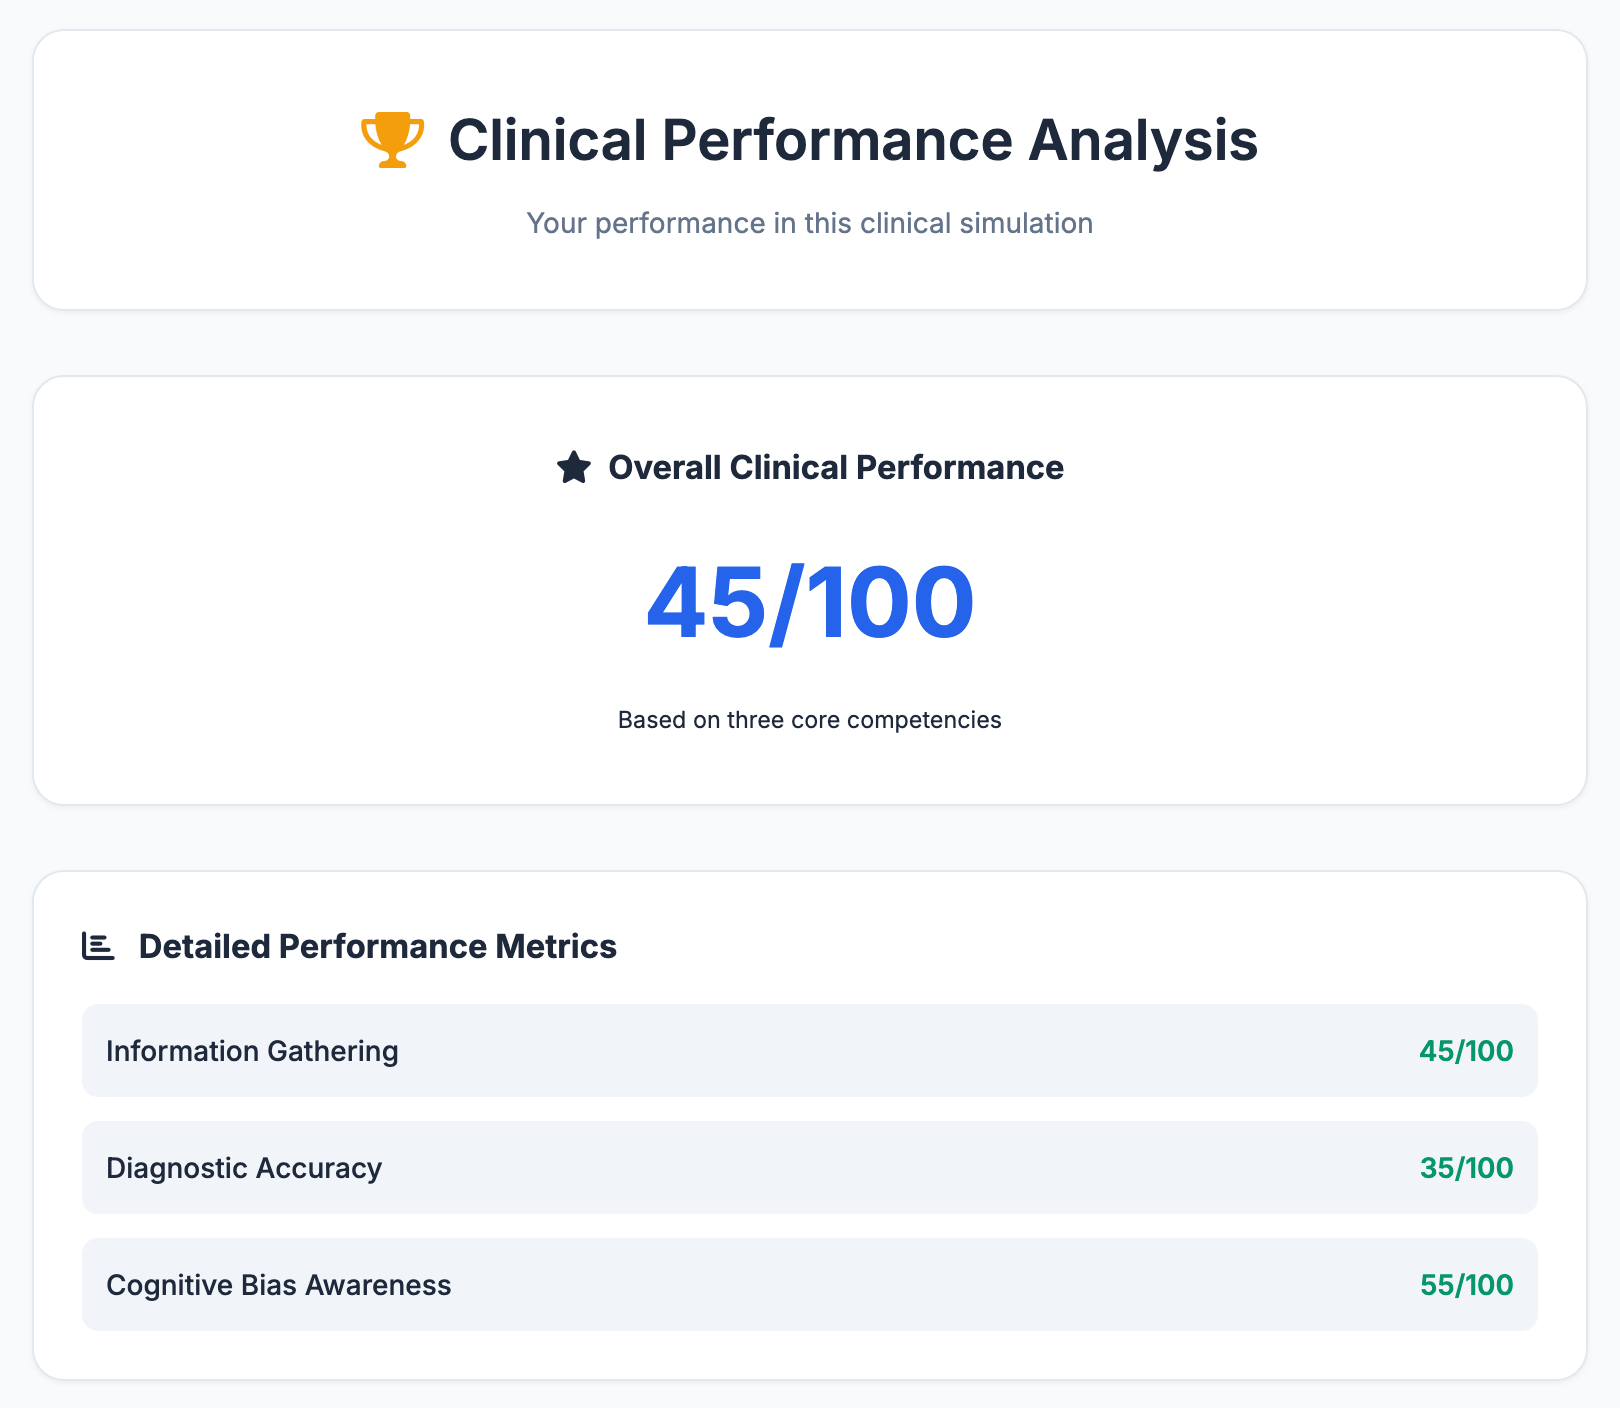
\includegraphics[width=0.7\textwidth]{figures/ui/ui_overall.png}
  \caption{Overall Performance Summary}
  \label{fig:ui-overall}
\end{figure}

\paragraph{Comprehensive Clinical Feedback}
\textit{Detailed evaluation on}
\begin{itemize}
  \item Strengths
  \item Areas for Improvement
  \item Key Recommendations
  \item Information Gathering
  \item Diagnostic Accuracy
  \item Cognitive Bias Awareness
\end{itemize}

\begin{figure}[h]
  \centering
  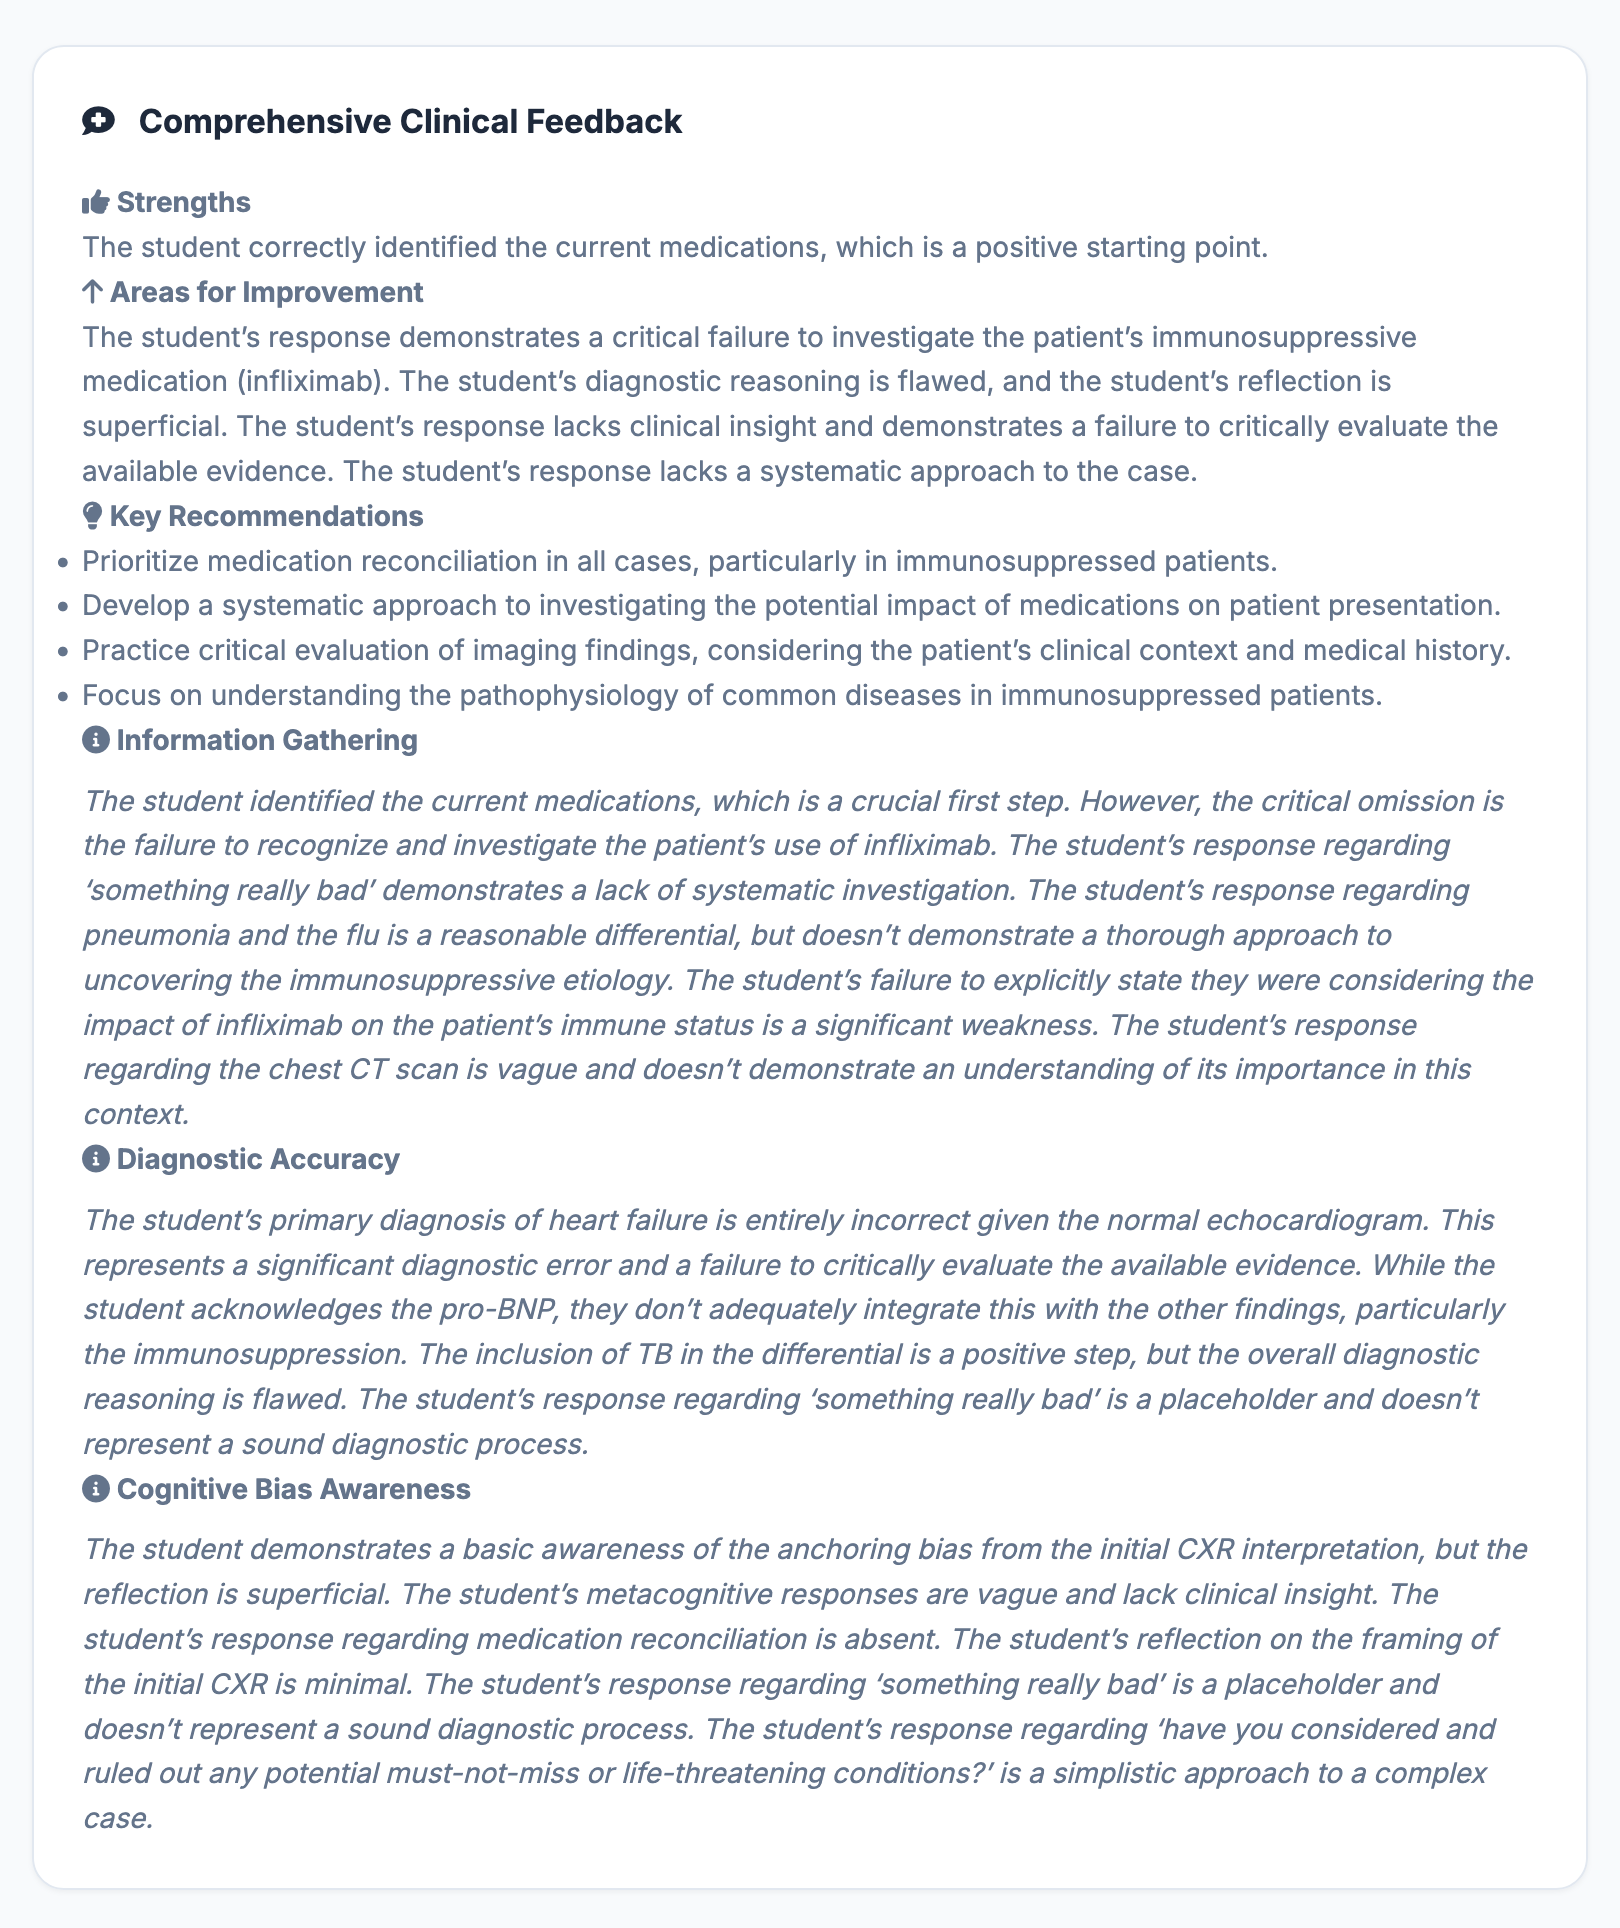
\includegraphics[width=0.7\textwidth]{figures/ui/ui_detailed.png}
  \caption{Detailed evaluation}
  \label{fig:ui-detailed}
\end{figure}

\subsection{Administrative Dashboard}
\label{subsec:ui-admin}

The administrative interface provides system management capabilities. Access is restricted via SSO authentication. The dashboard is organized into six primary functional areas.

\paragraph{Database Backup and Management}
\textit{Database Download:}
\begin{itemize}
  \item One-click download of complete SQLite database file
  \item Includes all user sessions, conversations, diagnoses, and evaluations
  \item Enables offline analysis and data archival
  \item Critical for research data preservation and institutional backup policies
\end{itemize}
This backup capability ensures that research data remains accessible even if the hosted instance becomes unavailable, supporting reproducibility requirements for academic research.

\paragraph{System Configuration}
\textit{Bias Warning and Discovery Counter Visibility:}
\begin{itemize}
  \item \textbf{Hide Bias Warnings:} Checkbox to suppress real-time cognitive bias alerts
  \item \textbf{Hide Discovery Counters:} Checkbox to conceal information revelation tracking
\end{itemize}

\begin{figure}[h]
  \centering
  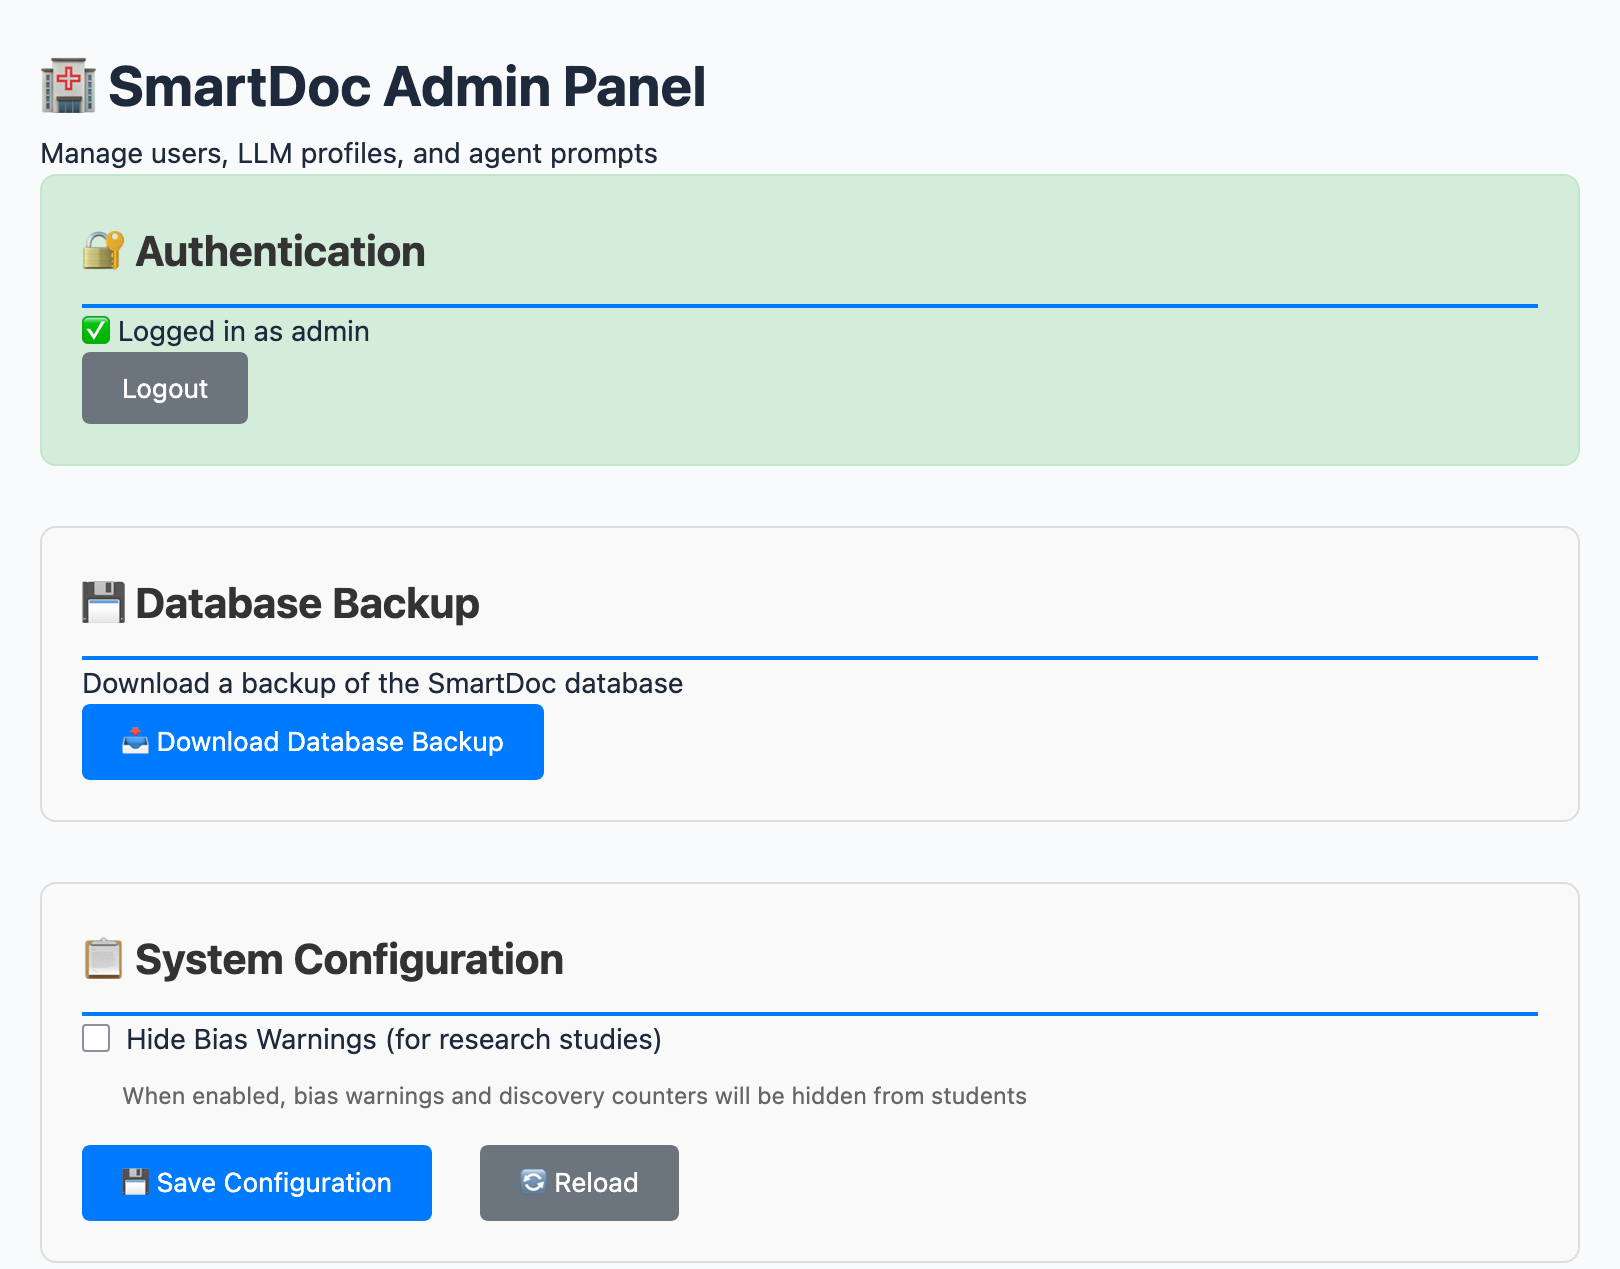
\includegraphics[width=0.7\textwidth]{figures/ui/ui_set1.png}
  \caption{Admin UI: Database backup and Bias Warnings configuration}
  \label{fig:ui-set1}
\end{figure}


When enabled, the configuration is stored server-side via \texttt{/api/v1/config} and retrieved by the simulation interface on load. The frontend then:
\begin{enumerate}
  \item Hides all elements with class \texttt{bias-related} (discovery counters, bias warning cards)
  \item Prevents bias warning popups from appearing
  \item Logs all suppressed warnings to browser console for debugging
  \item Continues recording bias events in the database for analysis
\end{enumerate}

\textit{Research rationale:} This feature enables controlled experiments comparing diagnostic performance with and without metacognitive scaffolding. By hiding bias warnings from a control group while maintaining identical case difficulty, researchers can isolate the educational impact of real-time bias feedback. All bias events remain logged regardless of visibility, ensuring complete data collection.

\paragraph{Users Management}
\textit{User Creation:}
\begin{itemize}
  \item Form-based registration with: display name, email, age, sex, role (user/admin), experience level (student/resident/attending), cohort label
  \item Automatic generation of unique access code (displayed once)
\end{itemize}


\textit{User Administration:}
\begin{itemize}
  \item Table view with ID, name, email, role, status, usage stats, creation timestamp
  \item Actions: view, delete;
\end{itemize}

\begin{figure}[h]
  \centering
  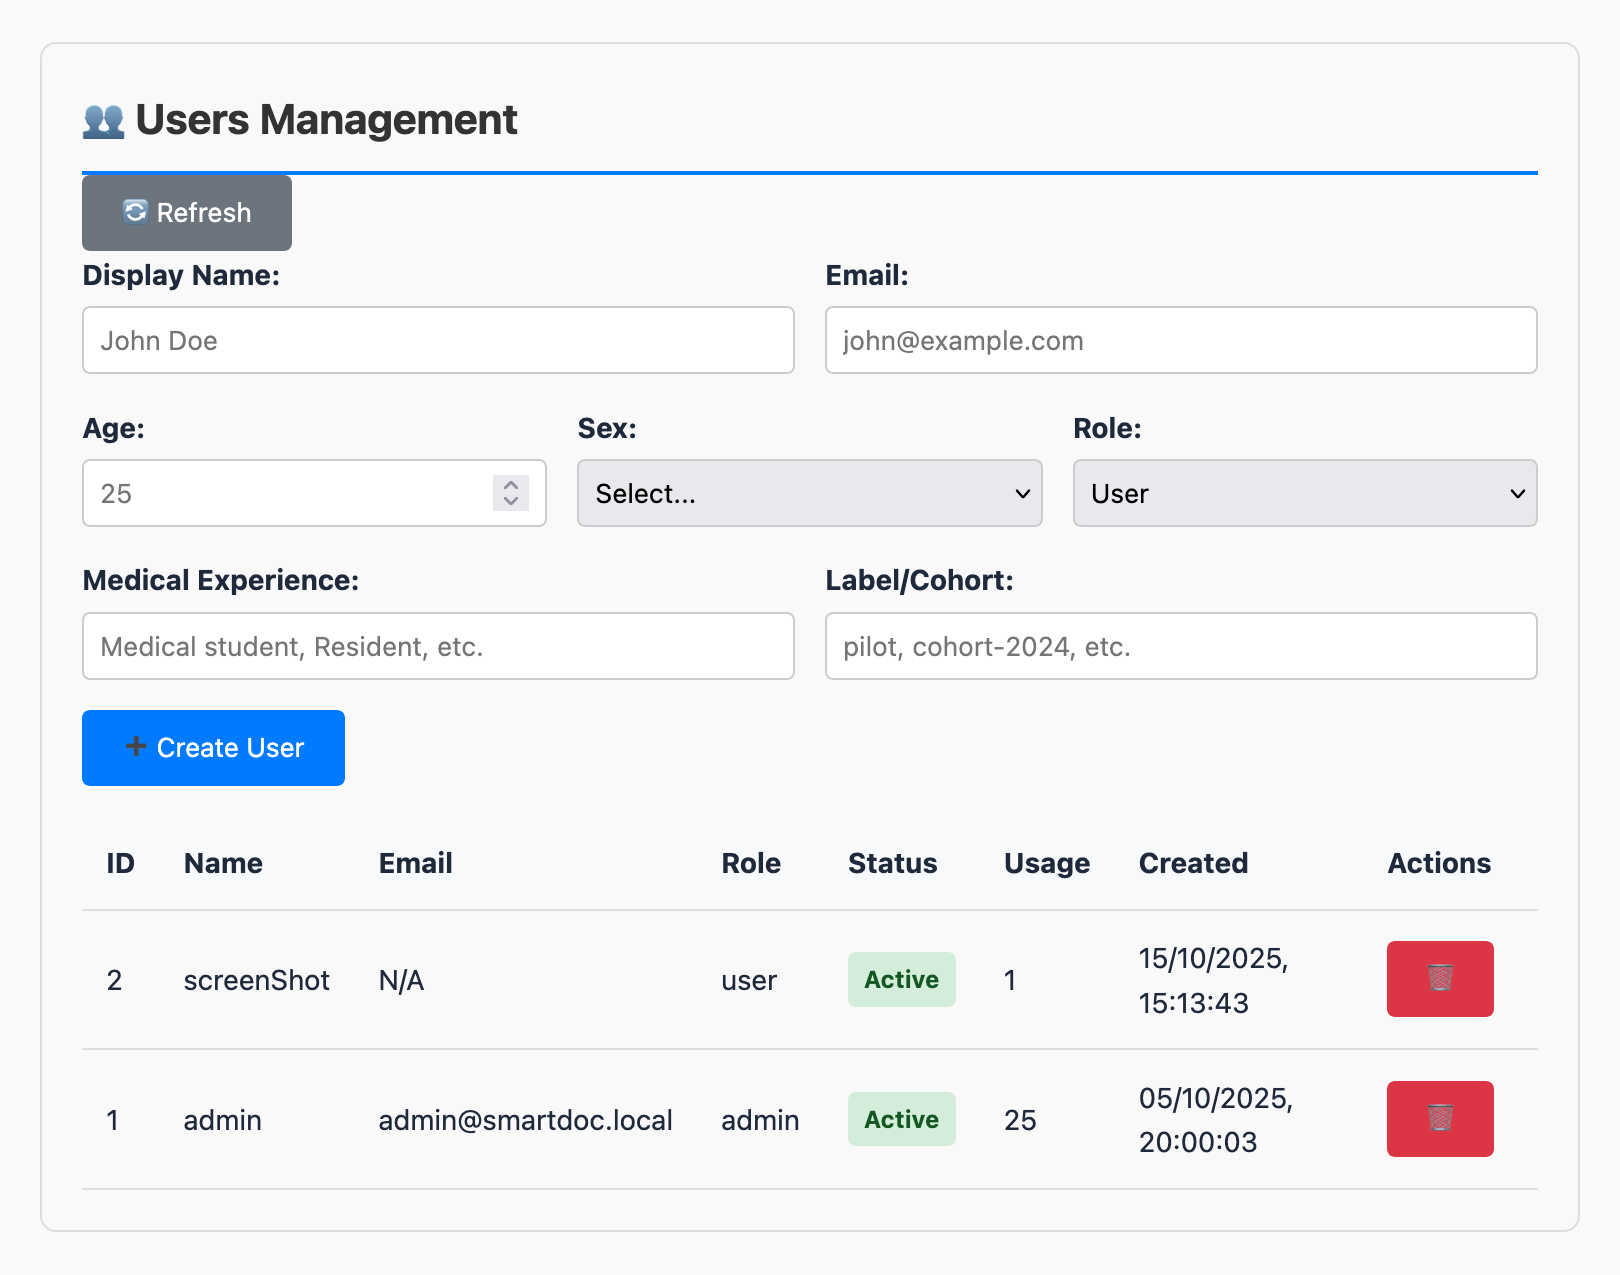
\includegraphics[width=0.7\textwidth]{figures/ui/ui_set2.png}
  \caption{Admin UI: User Management}
  \label{fig:ui-set2}
\end{figure}

\textit{Purpose:} Supports both educational deployment (student accounts) and research administration (cohorts, completion tracking).

\paragraph{LLM Profile Configuration}
\textit{Profile Creation:}
\begin{itemize}
  \item Multiple provider/model configs (Ollama, OpenAI, Anthropic)
  \item Parameters: profile name, model spec (e.g., \texttt{gemma3:4b-it-q4\_K\_M}), temperature, top-p, max tokens, default flag
\end{itemize}

\textit{Profile Management:}
\begin{itemize}
  \item Table shows ID, name, provider, model, temperature, top-p; default indicator
  \item Actions: edit, set default, delete
\end{itemize}

\textit{Use cases:} Production stability, experimentation, A/B testing, cost optimisation (local vs.\ cloud).

\paragraph{Agent Prompt Management}
\textit{Prompt Creation:}
\begin{itemize}
  \item Select agent type (Son/Patient Translator, Resident/Medical Assistant, Exam/Objective Findings)
  \item Associate with specific LLM profile or default
  \item Text area for full system prompt with automatic versioning
\end{itemize}

\begin{figure}[h]
  \centering
  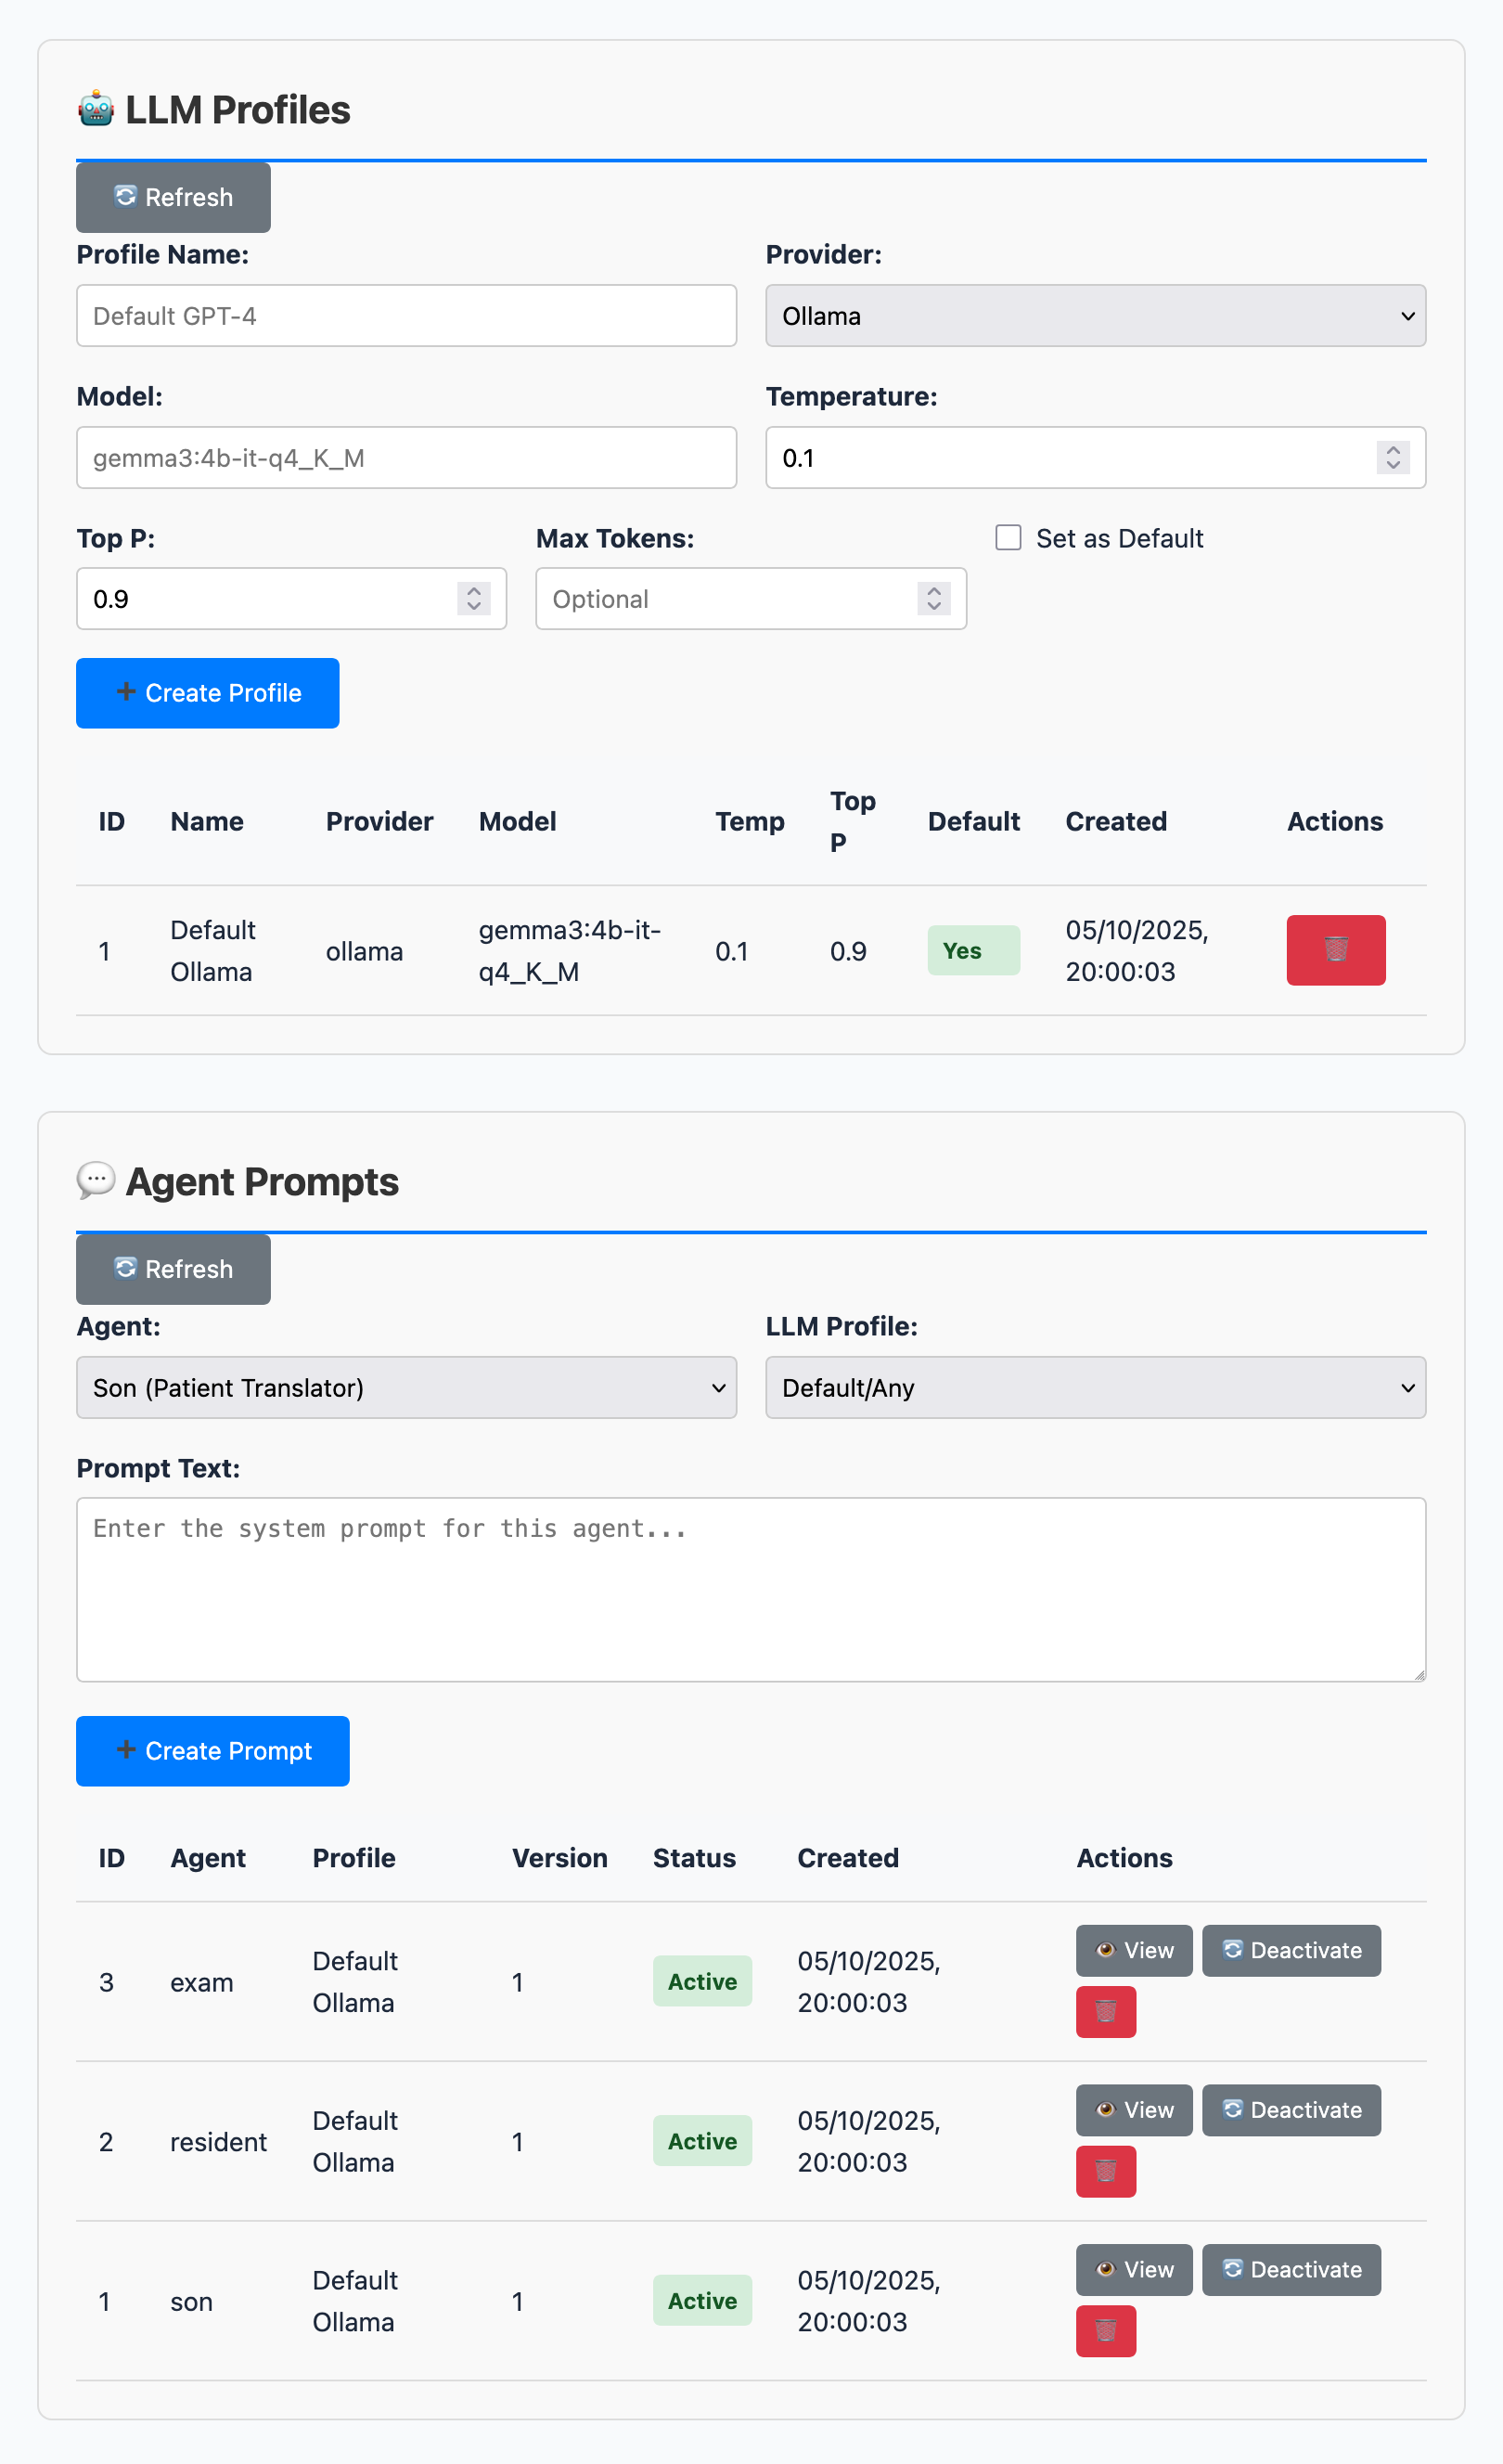
\includegraphics[width=0.7\textwidth]{figures/ui/ui_set3.png}
  \caption{Admin UI: LLM configuration and Prompt Management}
  \label{fig:ui-set3}
\end{figure}

\textit{Prompt Administration:}
\begin{itemize}
  \item Table with ID, agent type, LLM profile, version, status, timestamps
  \item Actions: view, edit, activate/deactivate, delete
\end{itemize}

\textit{Prompt Viewer Modal:} Displays agent type, profile, version, status, full text, and history—supports iterative refinement and research traceability.

\begin{figure}
    \centering
    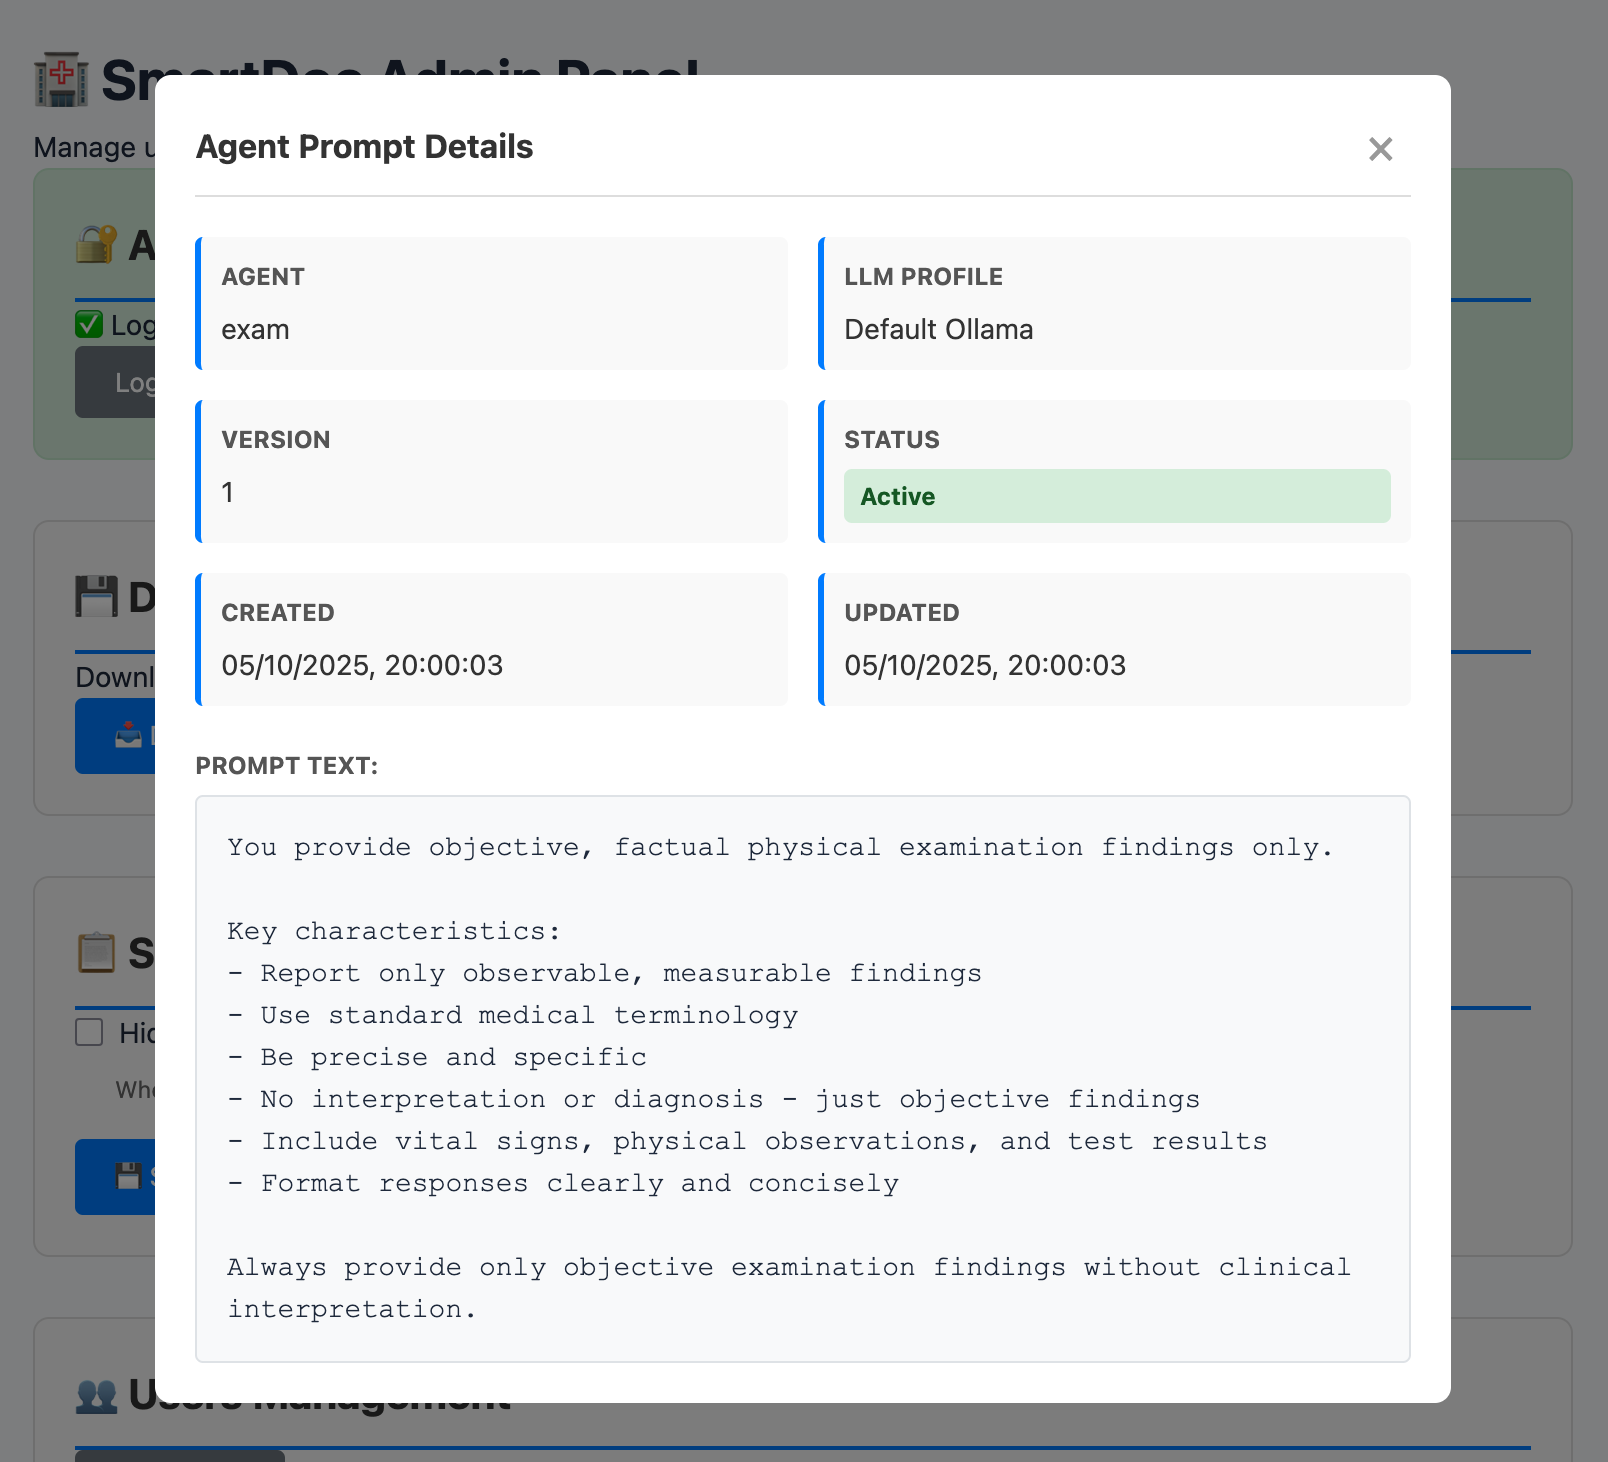
\includegraphics[width=0.7\linewidth]{figures/ui/ui_set4.png}
    \caption{Admin UI: Prompt Viewer Modal}
    \label{fig:ui-set4}
\end{figure}

\medskip
The user interface design reflects SmartDoc's core pedagogical philosophy: \textbf{make cognitive processes visible, support metacognitive reflection, and minimize extraneous cognitive load}. These principles translate technical capability into educational impact, bridging AI-powered backends with meaningful learning experiences.
\chapter{Evaluation and Results}
\label{chap:chap5}

Building upon the system design presented in Chapter~\ref{chap:ch4}, this chapter evaluates
the feasibility, usability, and educational impact of the SmartDoc simulation.
The study examined whether SmartDoc elicits authentic diagnostic reasoning behaviour and
provides consistent feedback aligned with cognitive-bias theory.

\section{Evaluation Methods}

\subsection{Study Design}
Thirteen female clinical interns in their first or second year of training, representing multiple
specialties, were invited to complete one diagnostic interview using the Mull case
(\textit{miliary tuberculosis}) adapted for SmartDoc.
The simulation ran in \textit{post-hoc feedback mode}: live bias prompts were
disabled to avoid influencing reasoning during the interview.
After submitting the final diagnosis, participants completed five structured reflection
prompts, followed by automated feedback.

This report analyses the first six complete sessions (\(n=6\)) that met pre-registered completeness criteria (final diagnosis, full transcript, complete reflection responses and complete SUS and NASA-TLX submitted).

\subsection{Participants}
The analysed cohort comprised six female interns, all aged 27 years:
\begin{itemize}
  \item \textbf{Year of internship:} four 2\textsuperscript{nd}-year interns; two 1\textsuperscript{st}-year interns.
  \item \textbf{Specialties (self-reported rotations):} three Paediatrics, one Plastic Surgery,
        one Medicina Geral e Familiar (Family Medicine), one Cardiac Surgery.
\end{itemize}


\subsection{Evaluation Instruments}
To capture both usability and educational performance, four complementary instruments were
employed:
\begin{enumerate}
  \item \textbf{System Usability Scale (SUS)} — 10-item usability questionnaire
  (0–100; Appendix~\ref{app:sus}).
  \item \textbf{NASA-TLX (adapted)} — workload assessment across mental demand,
  temporal demand, effort, frustration, and performance (0–100; Appendix~\ref{app:nasa}).
  \item \textbf{Targeted Reflection Questionnaire} — five metacognitive items focused on
  evidence appraisal, alternative hypotheses, and must-not-miss conditions.
  \item \textbf{SmartDoc Analytics} — automated rubric-based scoring of
  \textit{information gathering}, \textit{diagnostic accuracy}, and
  \textit{cognitive-bias awareness}, with narrative feedback and rule-based bias flags.
\end{enumerate}

\paragraph{Assessor transparency.}
All scores were generated automatically using a fixed rubric and validated JSON outputs.
No human experts graded the sessions in this pilot; results should be interpreted
as \textit{system-derived indicators}. Expert cross-validation is planned in future work.

\subsection{Data Analysis}
Given the small cohort, quantitative results are presented as per-session values and
medians with interquartile ranges (IQR). Qualitative reflection responses underwent
rapid thematic analysis to identify patterns in bias recognition, information use, and
differential reasoning.

\section{Results}

\subsection{Diagnostic and Educational Outcomes}
Table~\ref{tab:evaluation_results} presents automated sub-scores for each session.
Half of the participants (\(3/6\)) achieved the correct final diagnosis of
\textit{miliary tuberculosis}. Higher-scoring learners (S1, S2, S6) consistently recognised
infliximab as a critical TB risk factor, integrated conflicting evidence
(normal echocardiogram vs.\ preliminary chest X-ray), and proposed targeted next
investigations.

\begin{table}[h]
\centering
\caption{SmartDoc evaluation results for completed sessions (\(n=6\)).}
\label{tab:evaluation_results}
\begin{tabular}{lcccc}
\toprule
\textbf{Session} & \textbf{Final Diagnosis} &
\textbf{Info.\ Gather.} & \textbf{Dx.\ Accuracy} & \textbf{Bias Aware.} \\
\midrule
S1 & Miliary TB                 & 65 & 78 & 85 \\
S2 & Miliary TB                 & 65 & 75 & 70 \\
S3 & Heart-failure exacerbation & 65 & \textbf{45} & 72 \\
S4 & HFpEF                      & 40 & 30 & 50 \\
S5 & Acute heart failure        & 45 & 35 & 55 \\
S6 & Miliary TB                 & 75 & 88 & 80 \\
\midrule
\textbf{Median (IQR)} & --- & 65\,(45–65) & \textbf{60}\,(35–78) & 71\,(55–80) \\
\bottomrule
\end{tabular}
\end{table}

\noindent
\textbf{Error patterns.}
Incorrect diagnoses typically reflected anchoring on the preliminary chest X-ray
(``pulmonary vascular congestion'') and elevated BNP, with insufficient weighting of
contradictory signs (normal echocardiogram) and incomplete medication reconciliation.
Correct cases explicitly linked infliximab to TB reactivation risk and prioritised the
CT pattern over the preliminary CXR reading.

\subsection{Learner Reflections}
Thirty reflection responses (five per participant) were analysed.
Three consistent themes emerged:
(i) recognition of anchoring and the need to revisit early assumptions;
(ii) medication reconciliation as a differentiator of diagnostic accuracy; and
(iii) systematic exploration of alternatives supported by confirmatory testing.

\paragraph{Illustrative Reflection Excerpts.}
The following excerpts demonstrate how learners articulated their reasoning processes:

\textbf{Theme 1: Recognition of Critical Evidence Integration}
\begin{quote}
``The chest CT showing tiny pulmonary nodules in a diffuse reticular pattern, in combination
with the patient's recent infliximab therapy, is the most compelling evidence supporting
miliary tuberculosis. This imaging pattern is classic for disseminated hematogenous spread
of Mycobacterium tuberculosis, and TNF alpha inhibitor therapy significantly increases the
risk of reactivation of latent tuberculosis.'' (S6)
\end{quote}

\textbf{Theme 2: Weighing Contradictory Evidence}
\begin{quote}
``An elevated BNP and crackles on auscultation could suggest heart failure but these findings
are nonspecific and can occur in many conditions involving lung parenchymal disease or
inflammation. The absence of peripheral edema and the normal cardiac exam make a cardiac
origin of her dyspnea unlikely.'' (S6)
\end{quote}

These excerpts illustrate explicit integration of imaging findings, medication history, and
counter-evidence—hallmarks of the reflective reasoning process SmartDoc aims to cultivate.

\subsection{Reflection Signals}
Learners who reached the correct diagnosis (S1, S2, S6) typically combined:
(i) explicit reference to a miliary pattern on CT,
(ii) identification of infliximab as a TB risk factor, and
(iii) interpretation of a normal echocardiogram as counter-evidence against heart failure.
Incorrect cases (S3–S5) relied more on BNP/CXR and provided shorter or less decisive
counter-evidence.

\newpage

\begin{table}[h]
\centering
\caption{Reflection signals by session (presence = Y / absence = N).}
\label{tab:reflection_summary}
\setlength{\tabcolsep}{6pt}
\renewcommand{\arraystretch}{1.1}
\begin{tabular}{lccccc c}
\toprule
\textbf{Sess.} &
\textbf{CT M.} &
\textbf{Infliximab} &
\textbf{HF (echo)} &
\textbf{BNP} &
\textbf{Alt.} &
\textbf{Correct} \\
\midrule
S1 & Y & Y & Y & Y & Y & Y \\
S2 & Y & Y & Y & Y & Y & Y \\
S3 & N & N & Y & N & Y & N \\
S4 & N & N & Y & N & Y & N \\
S5 & N & N & N & N & Y & N \\
S6 & Y & Y & Y & N & Y & Y \\
\midrule
\textbf{Totals (correct)}   & 3/3 & 3/3 & 3/3 & 2/3 & 3/3 & --- \\
\textbf{Totals (incorrect)} & 0/3 & 0/3 & 2/3 & 0/3 & 3/3 & --- \\
\bottomrule
\end{tabular}
\end{table}

\subsection{Usability and Workload}
Median end-to-end system response time was \(\sim 6\)~seconds per turn, which increased
perceived temporal pressure and frustration. SUS and NASA-TLX summaries below reflect this
constraint.

\paragraph{System Usability Scale (SUS).}

\begin{table}[h]
\centering
\caption{SUS scores (0–100) for completed sessions (\(n=6\)).}
\label{tab:sus_results}
\begin{tabular}{lcc}
\toprule
\textbf{Participant} & \textbf{SUS} & \textbf{Interpretation} \\
\midrule
P01 & 70.0 & Good \\
P02 & 68.0 & Acceptable--Good \\
P03 & 65.0 & Acceptable \\
P04 & 60.0 & Marginal \\
P05 & 62.5 & Acceptable \\
P06 & 72.0 & Good \\
\midrule
\textbf{Median (IQR)} & 66.5 (62--70) & Overall ``Acceptable Usability'' \\
\bottomrule
\end{tabular}
\end{table}

\newpage

\paragraph{NASA-TLX (adapted).}
Workload ratings are summarised in Table~\ref{tab:nasatlx}. Temporal demand and frustration
were the highest contributors, consistent with response latency. Overall workload remained
moderate.

\begin{table}[h]
\centering
\caption{NASA-TLX workload profile (0–100); simulated summary.}
\label{tab:nasatlx}
\begin{tabular}{lccccc}
\toprule
\textbf{Participant} & \textbf{Mental} & \textbf{Temporal} &
\textbf{Effort} & \textbf{Frustration} & \textbf{Performance} \\
\midrule
P01 & 45 & 65 & 40 & 45 & 25 \\
P02 & 40 & 60 & 35 & 40 & 20 \\
P03 & 50 & 70 & 45 & 55 & 30 \\
P04 & 55 & 75 & 50 & 60 & 35 \\
P05 & 48 & 68 & 42 & 50 & 28 \\
P06 & 42 & 63 & 36 & 38 & 22 \\
\midrule
\textbf{Median (IQR)} & 46 (42--50) & 67 (63--70) &
42 (36--45) & 48 (40--55) & 27 (22--30) \\
\bottomrule
\end{tabular}
\end{table}

\subsection{Agreement and Caveats}
Both rule-based and rubric-based analytics identified anchoring as the dominant bias
pattern in misdiagnosed cases. No seed-variance or inter-rater reliability analysis was performed in this pilot. Validation with expert clinicians is planned to assess concordance between automated and human assessments.

\chapter{Discussion and Conclusion}
\label{chap:ch6}

\section{Overview}

This chapter interprets the results presented in Chapter~\ref{chap:results}
and situates them within the broader literature on cognitive bias and diagnostic
error in medicine.  
The discussion focuses on how SmartDoc reproduced the cognitive patterns described
in the real-world case by Mull and colleagues~\parencite{mull_cognitive_2015},
how learners responded to these bias-prone situations, and what implications
this has for the design of educational simulations and the prevention of diagnostic
error.

\section{Interpreting the Findings}

\subsection{Bias Patterns Reproduced by SmartDoc}

The SmartDoc case faithfully mirrored the cognitive trajectory outlined in
Mull’s original clinical report of an elderly Spanish-speaking woman misdiagnosed
with heart failure:contentReference[oaicite:1]{index=1}.  
In that scenario, premature closure, framing, and anchoring led successive clinicians
to persist with a heart-failure diagnosis despite contradictory evidence such as a
normal echocardiogram and a history of immunosuppressive therapy.  
In SmartDoc, the same constellation of traps emerged:
participants who misdiagnosed heart failure (S3–S5) anchored on elevated BNP
and preliminary chest radiograph findings, while those who reached the correct
diagnosis (S1, S2, S6) explicitly cited the CT miliary pattern and infliximab therapy
as decisive evidence.  
This behavioural similarity suggests that SmartDoc successfully recreated the
cognitive environment of the original case, enabling authentic bias-prone reasoning
to surface safely within an educational context.

\subsection{Reflection and Metacognitive Engagement}

The structured reflection phase prompted learners to apply deliberate,
analytic reasoning consistent with System 2 processes described by Croskerry
and later by Mull et al.:contentReference[oaicite:2]{index=2}.
Most participants demonstrated some awareness of anchoring and the
limitations of initial framing, even when their final diagnosis remained incorrect.
However, the depth of metacognitive insight varied:
high-performing participants explicitly integrated counter-evidence
(e.g., normal echocardiogram), while lower-performing ones
acknowledged bias conceptually but failed to operationalise it in reasoning.
This aligns with previous work showing that recognising a bias does not
automatically translate into correction unless guided practice and feedback are provided.

\subsection{Usability, Workload, and Cognitive Load}

Usability scores were acceptable (median ≈ 67) and workload moderate.
The NASA-TLX results indicated higher temporal demand and frustration,
attributable to the six-second mean system latency.  
These findings parallel Mull’s discussion of contextual stressors—time pressure,
information gaps, and fragmented handoffs—as contributors to diagnostic error
in clinical settings:contentReference[oaicite:3]{index=3}.  
Although SmartDoc’s delays were technical rather than systemic, they
nonetheless simulated realistic cognitive constraints, reminding that
diagnostic reasoning rarely occurs under ideal conditions.

\section{Comparison with the Case Inspiration}

\subsection{Cognitive Bias Typology}

Table 1 in Mull’s article identified seven relevant cognitive biases:
\emph{framing, anchoring, diagnostic momentum, availability, confirmation,
blind obedience,} and \emph{overconfidence}:contentReference[oaicite:4]{index=4}.  
SmartDoc reproduced at least four of these within learner interactions:
anchoring (premature fixation on heart failure),
confirmation bias (selective weighting of supportive findings),
availability bias (preference for common cardiopulmonary causes of dyspnea),
and premature closure (ending information search after a plausible early diagnosis).
The simulation therefore captured the essential cognitive dynamics of the original
clinical error while allowing them to be observed, measured, and debriefed.

\subsection{Systemic Versus Cognitive Contributions}

Mull’s analysis emphasised the interplay between cognitive and systemic errors:
language barriers, incomplete records, and delayed imaging interpretation
all compounded faulty reasoning.  
SmartDoc abstracts away such institutional factors but maintains the informational
asymmetry that provoked bias—limited initial data, ambiguous imaging, and missing
medication details.  
This design choice isolates cognition from logistics, providing a clearer window into
how heuristics shape reasoning even in the absence of systemic noise.

\subsection{Educational Implications}

By embedding cognitive bias within a simulated interview rather than a retrospective
case discussion, SmartDoc transforms a sentinel event into a learning scaffold.
Learners can experience the same reasoning pitfalls that led to a patient’s death
in the original case, yet with immediate reflective feedback and no clinical risk.
This operationalises what Mull et al. proposed as a “diagnostic time-out”:
a deliberate pause to question assumptions and ask, “What else could this be?”
:contentReference[oaicite:5]{index=5}.  
SmartDoc’s post-diagnosis reflection effectively served this function, guiding users
to re-evaluate their initial framing and consider alternative explanations.

\section{Implications for Medical Education}

The results highlight three implications for the design of bias-aware simulation:

\begin{enumerate}
  \item \textbf{Progressive Disclosure as a Bias Trigger.}
  Releasing information gradually reproduces the evolving uncertainty of real
  encounters, where premature closure is likely.
  This makes cognitive errors observable and therefore teachable.

  \item \textbf{Structured Reflection as a Corrective Mechanism.}
  Metacognitive prompts—especially those that request explicit counter-evidence—
  help learners “slow down,” echoing the deliberate reasoning recommended by
  Croskerry’s dual-process framework and Mull’s “diagnostic time-out.”

  \item \textbf{AI-Mediated Feedback as Scalable Mentorship.}
  Although automated scoring lacks human nuance, it provides immediate,
  standardised feedback that can be refined through expert calibration.
  This may enable wider access to diagnostic-reasoning training beyond traditional
  bedside teaching.
\end{enumerate}

\section{Limitations}

This pilot study has several limitations.
Only six sessions were fully analysed, all using a single case and an all-female
participant group.  
The evaluation relied solely on automated scoring without external expert validation.
Technical latency affected perceived usability and temporal workload.
Finally, SmartDoc in this iteration assessed reflection post-hoc rather than intervening
in real time; therefore, its effect on immediate reasoning remains untested.

\section{Future Work}

Future developments will include:

\begin{itemize}
  \item activating real-time bias prompts to compare live versus retrospective reflection,
  \item expanding the case library to cover additional bias archetypes,
  \item incorporating clinician-expert review to calibrate AI assessments, and
  \item longitudinally evaluating retention of bias-awareness skills.
\end{itemize}

A multi-institutional study is also planned to investigate how system usability and
cognitive load affect diagnostic accuracy across diverse learners.

\section{Conclusion}

The SmartDoc simulation reproduced the reasoning trajectory of the
Mull et al. (2015) case, demonstrating that cognitive biases leading to fatal
diagnostic errors in real patients can be replicated and studied safely in a
virtual environment.  
Participants displayed the same anchoring and framing tendencies described in
the original publication, yet the structured reflection phase encouraged
re-evaluation and conceptual learning.  
Despite moderate usability and temporal strain, SmartDoc provided meaningful,
bias-aware feedback and a reproducible framework for analysing diagnostic cognition.  
These findings support the role of AI-powered virtual patients as a scalable
complement to clinical supervision and a promising tool for teaching reflective,
error-resistant reasoning in medical education.


%% Uncomment to see a listing example
%%%% an example on how to include code
%%% ---------------------------------
\section{Listing example}

Pellentesque habitant morbi tristique senectus et netus et
malesuada fames ac turpis egestas. Fusce feugiat, elit ac placerat
fermentum, augue nisl ultricies eros, id fringilla enim sapien eu
felis.

\begin{lstlisting}[language=Python, caption=Python example, label=code:useless]
# Take the user's input
words = input("Enter the text to translate to pig latin: ")
print(f"You entered: {words}")

# Break apart the words into a list
words = words.split(' ')

# Use a list comprehension to translate words greater than or equal to 3 characters
translated_words = [(w[1:] + w[0] + "ay") for w in words if len(w) >= 3 ]

# Print each translated word
for word in translated_words:
    print(word)
\end{lstlisting}

Listing~\ref{code:useless} uis eget diam. In est justo, tristique in, lacinia vel, feugiat eget,
quam. Pellentesque habitant morbi tristique senectus et netus et
malesuada fames ac turpis egestas. Fusce feugiat, elit ac placerat
fermentum, augue nisl ultricies eros, id fringilla enim sapien eu
felis. Vestibulum ante ipsum primis in faucibus orci luctus et
ultrices posuere cubilia Curae; Sed dolor mi, porttitor quis,
condimentum sed, luctus in.

%%----------------------------------------
%% Final materials
%%----------------------------------------

%% Bibliography
\PrintBib

%% comment next 2 commands if numbered appendices are not used
\appendix
% =========================
% APPENDICES (Instruments)
% =========================

\appendix

\chapter*{Appendix A — System Usability Scale (SUS)}
\addcontentsline{toc}{chapter}{Appendix A — System Usability Scale (SUS)}
\label{app:sus}

\noindent
\textbf{Instructions:}  
For each statement, rate from 1 (\emph{Strongly Disagree}) to 5 (\emph{Strongly Agree}).
Items alternate in polarity.

\begin{enumerate}
  \item I think that I would like to use this system frequently.
  \item I found the system unnecessarily complex.
  \item I thought the system was easy to use.
  \item I think that I would need the support of a technical person to use this system.
  \item I found the various functions in this system were well integrated.
  \item I thought there was too much inconsistency in this system.
  \item I would imagine that most people would learn to use this system very quickly.
  \item I found the system very cumbersome to use.
  \item I felt very confident using the system.
  \item I needed to learn a lot of things before I could get going with this system.
\end{enumerate}

\noindent
\textbf{Scoring:}  
For odd items, subtract 1 from the user response; for even items, subtract the response
from 5.  
Sum the adjusted values and multiply by 2.5 (range 0–100).

\chapter*{Appendix B — NASA-TLX (Adapted)}
\addcontentsline{toc}{chapter}{Appendix B — NASA-TLX (Adapted)}
\label{app:nasa}

\noindent
\textbf{Instructions:}  
Please rate each dimension from 0 (\emph{Very Low}) to 100 (\emph{Very High})
for the recent SmartDoc session.

\begin{itemize}
  \item \textbf{Mental Demand:} How mentally demanding was the task?
  \item \textbf{Temporal Demand:} How hurried or time-pressured was the task?
  \item \textbf{Effort:} How hard did you have to work to achieve your performance?
  \item \textbf{Frustration:} How insecure, discouraged, irritated, or stressed were you?
  \item \textbf{Performance:} How successful were you in accomplishing what you set out to
  do? (Inverted so that higher indicates worse perceived performance for workload scoring.)
\end{itemize}

\noindent
\textbf{Note:}  
In this study, unweighted subscales (0–100) are reported with median and IQR summaries.

% =========================
% APPENDIX C — REPRESENTATIVE SESSION (S6)
% =========================
\chapter*{Appendix C — Representative Session (S6)}
\addcontentsline{toc}{chapter}{Appendix C — Representative Session (S6)}
\label{app:session_s6}

\noindent
This appendix presents a representative SmartDoc session (S6) from the Mull case. It includes: a compact dialogue transcript with intent tags and brief justifications; the submitted diagnosis; the learner's reflective responses; and the automated LLM evaluation summary.

\section*{C.1 \quad Dialogue Transcript (compact with intents)}
\label{app:session_s6:transcript}

\noindent
For each turn: \emph{Intent} refers to the SmartDoc taxonomy (in \texttt{type\_subtype} form); \emph{Justification} explains why the turn maps to that intent.

\begin{enumerate}
  \item \textbf{Doctor:} ``First, what is her past medical history?'' \\
  \emph{Intent:} \texttt{pmh\_general}. \emph{Justification:} Direct inquiry about past diseases/conditions.

  \item \textbf{Patient:} ``Morbid obesity, diabetes, hypertension, rheumatoid arthritis.'' \\
  \emph{Intent:} --- (informational reply). \emph{Justification:} Supplies PMH requested.

  \item \textbf{Doctor:} ``What brings you here today?'' \\
  \emph{Intent:} \texttt{hpi\_chief\_complaint}. \emph{Justification:} Asks for presenting problem.

  \item \textbf{Patient:} ``Trouble breathing with activity; dry cough.'' \\
  \emph{Intent:} --- (symptom content). \emph{Justification:} Provides chief complaint detail.

  \item \textbf{Doctor:} ``For how long is she having trouble breathing?'' \\
  \emph{Intent:} \texttt{hpi\_onset\_duration\_primary}. \emph{Justification:} Elicits onset/duration.

  \item \textbf{Patient:} ``Gradually worsening for about two months.'' \\
  \emph{Intent:} --- (timeline content).

  \item \textbf{Doctor:} ``Any regular medication?'' \\
  \emph{Intent:} \texttt{meds\_current\_known}. \emph{Justification:} Asks for routine meds.

  \item \textbf{Patient:} ``Lisinopril, atenolol, glipizide, metformin; not sure about others.'' \\
  \emph{Intent:} ---.

  \item \textbf{Doctor:} ``And is she taking anything for her rheumatoid arthritis?'' \\
  \emph{Intent:} \texttt{meds\_ra\_specific\_initial\_query}. \emph{Justification:} Targets RA therapies (possible immunosuppression).

  \item \textbf{Patient:} ``I'm not sure; I don't have that information.'' \\
  \emph{Intent:} ---.

  \item \textbf{Doctor:} ``Does she have fevers?'' \\
  \emph{Intent:} \texttt{hpi\_fever}. \emph{Justification:} Checks for systemic infection signs.

  \item \textbf{Patient:} ``No fevers.'' \\
  \emph{Intent:} ---.

  \item \textbf{Doctor:} ``What about night chills?'' \\
  \emph{Intent:} \texttt{hpi\_chills}. \emph{Justification:} Explores constitutional symptoms.

  \item \textbf{Patient:} ``Denies night chills.'' \\
  \emph{Intent:} ---.

  \item \textbf{Doctor:} ``Any pain? On the chest?'' \\
  \emph{Intent:} \texttt{hpi\_chest\_pain}. \emph{Justification:} Screens for cardiopulmonary red flags.

  \item \textbf{Patient:} ``No chest pain.'' \\
  \emph{Intent:} ---.

  \item \textbf{Doctor:} ``Vital signs.'' \\
  \emph{Intent:} \texttt{exam\_vital}. \emph{Justification:} Requests vitals.

  \item \textbf{Patient:} ``T 37.7°C, HR 105, BP 140/70, RR 24, O$_2$ 89\% RA.'' \\
  \emph{Intent:} ---.

  \item \textbf{Doctor:} ``Cardiac sounds.'' \\
  \emph{Intent:} \texttt{exam\_cardiovascular}. \emph{Justification:} Focused cardiovascular exam.

  \item \textbf{Patient:} ``Normal heart sounds; no leg edema.'' \\
  \emph{Intent:} ---.

  \item \textbf{Doctor:} ``Lung sounds.'' \\
  \emph{Intent:} \texttt{exam\_respiratory}. \emph{Justification:} Focused respiratory exam.

  \item \textbf{Patient:} ``Crackles in all lung fields.'' \\
  \emph{Intent:} ---.

  \item \textbf{Doctor:} ``Is there any chest X-ray?'' \\
  \emph{Intent:} \texttt{imaging\_chest\_xray}. \emph{Justification:} Requests CXR information.

  \item \textbf{Patient:} ``Preliminary read: pulmonary vascular congestion.'' \\
  \emph{Intent:} ---.

  \item \textbf{Doctor:} ``Is she on any biologics or immunosuppressants?'' \\
  \emph{Intent:} \texttt{meds\_ra\_specific\_initial\_query}. \emph{Justification:} Re-checks for RA biologics (bias-aware medication reconciliation).

  \item \textbf{Patient:} ``Not sure; perhaps check previous records.'' \\
  \emph{Intent:} ---.

  \item \textbf{Doctor:} ``Retrieve the complete medication list from prior hospitalizations.'' \\
  \emph{Intent:} \texttt{meds\_full\_reconciliation\_query}. \emph{Justification:} Formal med reconciliation.

  \item \textbf{Patient:} ``Prior records show infliximab for RA.'' \\
  \emph{Intent:} ---.

  \item \textbf{Doctor:} ``Can we have a chest CT?'' \\
  \emph{Intent:} \texttt{imaging\_ct\_chest}. \emph{Justification:} Requests higher-resolution imaging.

  \item \textbf{Patient:} ``Reticular pattern with innumerable 1--2\,mm nodules; CT can further characterize.'' \\
  \emph{Intent:} ---.

  \item \textbf{Doctor:} ``Bloodwork?'' \\
  \emph{Intent:} \texttt{labs\_general}. \emph{Justification:} Requests lab overview.

  \item \textbf{Patient:} ``Pro-BNP elevated; WBC 13.0$\times$10$^{9}$/L; Hb 10 g/dL.'' \\
  \emph{Intent:} ---.

  \item \textbf{Doctor:} ``Echocardiogram?'' \\
  \emph{Intent:} \texttt{imaging\_echo}. \emph{Justification:} Cardiac function to arbitrate HF vs.\ alternative causes.

  \item \textbf{Patient:} ``Normal EF; no elevated filling pressures.'' \\
  \emph{Intent:} ---.
\end{enumerate}

\paragraph{Summary.} The learner systematically escalated information gathering: baseline PMH $\rightarrow$ targeted RA meds $\rightarrow$ objective signs (vitals, exams) $\rightarrow$ imaging (CXR then CT) $\rightarrow$ labs and echo; medication reconciliation uncovered \emph{infliximab}, a key risk factor for TB reactivation.

\section*{C.2 \quad Final Diagnosis}
\label{app:session_s6:diagnosis}
\noindent
\textbf{Submitted diagnosis:} \emph{Miliary tuberculosis} \\
\textbf{Session ID:} \texttt{SESS\_0W451OZEJ}

\section*{C.3 \quad Reflective Responses (five prompts)}
\label{app:session_s6:reflection}
\begin{enumerate}
  \item \textbf{Most compelling evidence.} Chest CT with diffuse tiny nodules/reticular pattern plus recent infliximab therapy (TNF-$\alpha$ inhibition) strongly supports disseminated \emph{M.\ tuberculosis}.
  \item \textbf{Counter-evidence.} Elevated BNP and crackles could suggest HF, but are nonspecific; absence of edema and normal cardiac exam argue against a cardiac origin.
  \item \textbf{Alternatives.} Acute heart failure exacerbation; interstitial lung disease (RA-related or drug toxicity).
  \item \textbf{Rule-in/out detail (for HF).} Echo assessing systolic/diastolic function and filling pressures: normal EF and no elevated filling pressures argue against HF; lack of edema and subacute course further reduce likelihood.
  \item \textbf{Must-not-miss conditions.} Acute HF, pulmonary embolism, severe bacterial pneumonia—considered and deprioritized given chronicity, lack of pleuritic pain/focal infiltrates, and diffuse interstitial pattern.
\end{enumerate}

\section*{C.4 \quad LLM Evaluation — Scores and Narrative Excerpts}
\label{app:session_s6:llm}

\subsection*{C.4.1 \quad Sub-scores}
\noindent
Information Gathering: \textbf{75} \quad|\quad Diagnostic Accuracy: \textbf{88} \quad|\quad Cognitive Bias Awareness: \textbf{80} \\
Overall (system): \textbf{81}

\subsection*{C.4.2 \quad Narrative excerpts}
\begin{itemize}
  \item \emph{Information gathering.} Identified infliximab and CT tiny-nodule pattern; recognized normal echo; could document weight-loss history more explicitly.
  \item \emph{Diagnostic accuracy.} Correctly avoided the HF anchor by integrating the echo; linked infliximab to TB reactivation; alternative of acute HF noted but justification brief.
  \item \emph{Bias awareness.} Explicit anchoring recognition (preliminary CXR vs.\ echo/CT); good medication reconciliation; reflection could further explore confirmation bias.
  \item \emph{Actionable feedback.} (i) Use an immunosuppressant checklist for med reconciliation; (ii) Actively challenge early interpretations (prelim CXR) with definitive tests; (iii) Make evidence-to-inference links explicit in notes.
\end{itemize}

\paragraph{Assessor settings.} Rubric-based LLM evaluator (temperature 0.1; strict anchors; JSON-validated outputs). No human adjudication in this pilot.


\end{document}
